% \documentclass[12pt,a4paper,titlepage]{book}
\documentclass[12pt,a4paper,titlepage]{article}
% \documentclass[12pt,a4paper,titlepage,final]{book}
% \documentclass[12pt,a4paper,titlepage,brazil,portugues]{book}
%--------------------------------------------------------------------
% \usepackage[left=2.5cm,right=2.5cm,top=4cm,bottom=2.5cm]{geometry}
\usepackage[left=1.5cm,right=3.5cm,top=4cm,bottom=2.5cm]{geometry}
% \documentclass[a4paper]{article}
% \documentclass[
  % % border={0pt 0pt 0pt 0pt} % left bottom right top
% ]{standalone}

%--------------------------------------------------------------------
% \usepackage[left=1.5cm,right=3.5cm,top=4cm,bottom=2.5cm]{geometry}
%--------------------------------------------------------------------
% Pacotes usados {{
\usepackage[utf8]{inputenc}
\usepackage[T1]{fontenc}
\usepackage{amsmath,amssymb,amsfonts,amstext,textcomp}         % permite simbolos matematicos
\usepackage{bm}                                                % negrito em letras gregas
\usepackage{mathrsfs}                                          % permite o uso de letras trabalhadas
\usepackage{amsthm}
\usepackage{pgf}
\usepackage{graphicx}
\usepackage{float} % Allows putting an [H] in \begin{figure} to specify the exact location of the figure
\usepackage{color}
\usepackage{xcolor}
\definecolor{myOrange}{rgb}{1,0.5,0}
% \definecolor{myOrange}{rgb}{1,0.5,0}
\usepackage{booktabs}                                          % Tabelas com qualidade de publicao
\usepackage{indentfirst}
\usepackage{rotating}
\usepackage{braket}
\usepackage[ruled,vlined]{algorithm2e}                         % Para algoritmos (melhor que o outro)
\usepackage{multirow}
\usepackage{fancyhdr}
\usepackage{makeidx}
\usepackage{setspace}
\usepackage[colorlinks,citecolor=blue]{hyperref}               % tirar [colorlinks] para imprimir
% \usepackage{autonum}                                         % Mostra numeracao somente em eq citadas
\usepackage{mathtools}
\mathtoolsset{showonlyrefs=true}                               % Mostra numeracao somente em eq citadas
\usepackage{ae}
\usepackage[below]{placeins}
\usepackage{flafter}
\usepackage{pxfonts}
% \usepackage{subfigure}
\usepackage{appendix}
\usepackage{listings}                                          % para cdigo fonte
\usepackage[symbol]{footmisc}                                  % Mudando marcadores do footnote
% Tikz
\usepackage{tikz}
\usepackage{pgfplots}
\usetikzlibrary{shapes,arrows,calc,automata,positioning}
\usetikzlibrary{plotmarks}    % marcas nos graficos
\usetikzlibrary{arrows.meta}  % estilos de setas

\usepgfplotslibrary{patchplots}

\usepackage{soul}                                              % para highlighth (todonotes)
\usepackage{natbib}                                            % para usar citep, etc...
\usepackage{subfig}                                            % para subfiguras

\pgfplotsset{compat=newest}
%% the following commands are needed for some matlab2tikz features
\usepackage{grffile}   % Permite usar carc. esp. em nomes de arq
\usepackage{amsmath}   % Enhance-ments for improving mathematical formulas



\begin{document}
\thispagestyle{empty}
  \begin{figure}[htpb]
    \small
    % Created by tikzDevice version 0.12.3.1 on 2021-05-12 13:53:03
% !TEX encoding = UTF-8 Unicode
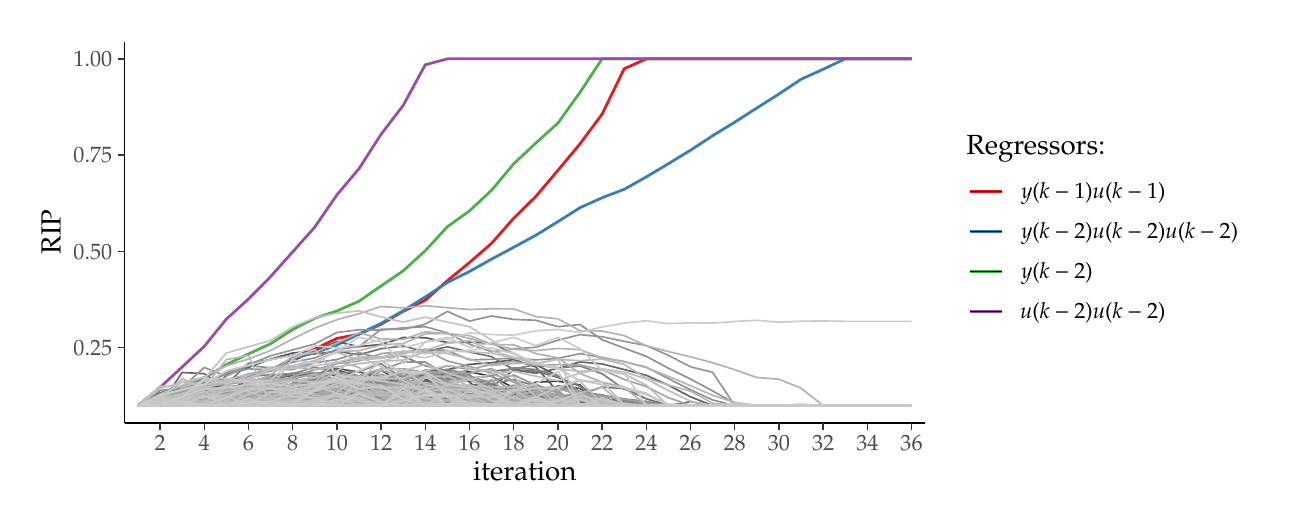
\begin{tikzpicture}[x=1pt,y=1pt]
\definecolor{fillColor}{RGB}{255,255,255}
\path[use as bounding box,fill=fillColor,fill opacity=0.00] (0,0) rectangle (455.24,170.72);
\begin{scope}
\path[clip] (  0.00,  0.00) rectangle (455.24,170.72);
\definecolor{drawColor}{RGB}{255,255,255}
\definecolor{fillColor}{RGB}{255,255,255}

\path[draw=drawColor,line width= 0.5pt,line join=round,line cap=round,fill=fillColor] (  0.00,  0.00) rectangle (455.24,170.72);
\end{scope}
\begin{scope}
\path[clip] ( 35.05, 27.90) rectangle (324.17,165.72);
\definecolor{fillColor}{RGB}{255,255,255}

\path[fill=fillColor] ( 35.05, 27.90) rectangle (324.17,165.72);
\definecolor{drawColor}{RGB}{228,26,28}

\path[draw=drawColor,line width= 1.0pt,line join=round] ( 39.84, 34.16) --
	( 47.83, 35.27) --
	( 55.82, 37.02) --
	( 63.80, 39.31) --
	( 71.79, 42.32) --
	( 79.78, 43.87) --
	( 87.76, 47.21) --
	( 95.75, 50.26) --
	(103.74, 54.59) --
	(111.72, 58.42) --
	(119.71, 59.93) --
	(127.70, 63.56) --
	(135.68, 68.19) --
	(143.67, 72.23) --
	(151.66, 79.29) --
	(159.64, 85.85) --
	(167.63, 92.80) --
	(175.62,101.85) --
	(183.60,109.72) --
	(191.59,119.15) --
	(199.58,128.74) --
	(207.56,139.49) --
	(215.55,155.87) --
	(223.54,159.45) --
	(231.52,159.45) --
	(239.51,159.45) --
	(247.50,159.45) --
	(255.48,159.45) --
	(263.47,159.45) --
	(271.46,159.45) --
	(279.45,159.45) --
	(287.43,159.45) --
	(295.42,159.45) --
	(303.41,159.45) --
	(311.39,159.45) --
	(319.38,159.45);
\definecolor{drawColor}{RGB}{55,126,184}

\path[draw=drawColor,line width= 1.0pt,line join=round] ( 39.84, 34.16) --
	( 47.83, 35.33) --
	( 55.82, 39.78) --
	( 63.80, 40.43) --
	( 71.79, 42.37) --
	( 79.78, 45.39) --
	( 87.76, 46.74) --
	( 95.75, 51.19) --
	(103.74, 53.23) --
	(111.72, 55.99) --
	(119.71, 60.05) --
	(127.70, 63.86) --
	(135.68, 68.43) --
	(143.67, 73.40) --
	(151.66, 78.64) --
	(159.64, 82.62) --
	(167.63, 87.08) --
	(175.62, 91.36) --
	(183.60, 95.69) --
	(191.59,100.61) --
	(199.58,105.66) --
	(207.56,109.25) --
	(215.55,112.31) --
	(223.54,116.79) --
	(231.52,121.56) --
	(239.51,126.42) --
	(247.50,131.67) --
	(255.48,136.55) --
	(263.47,141.68) --
	(271.46,146.74) --
	(279.45,152.07) --
	(287.43,155.69) --
	(295.42,159.45) --
	(303.41,159.45) --
	(311.39,159.45) --
	(319.38,159.45);
\definecolor{drawColor}{RGB}{77,175,74}

\path[draw=drawColor,line width= 1.0pt,line join=round] ( 39.84, 34.16) --
	( 47.83, 38.59) --
	( 55.82, 40.78) --
	( 63.80, 43.99) --
	( 71.79, 49.00) --
	( 79.78, 52.82) --
	( 87.76, 56.50) --
	( 95.75, 61.64) --
	(103.74, 65.70) --
	(111.72, 68.34) --
	(119.71, 71.86) --
	(127.70, 77.38) --
	(135.68, 82.85) --
	(143.67, 90.11) --
	(151.66, 98.78) --
	(159.64,104.51) --
	(167.63,111.97) --
	(175.62,121.52) --
	(183.60,129.00) --
	(191.59,136.21) --
	(199.58,147.35) --
	(207.56,159.45) --
	(215.55,159.45) --
	(223.54,159.45) --
	(231.52,159.45) --
	(239.51,159.45) --
	(247.50,159.45) --
	(255.48,159.45) --
	(263.47,159.45) --
	(271.46,159.45) --
	(279.45,159.45) --
	(287.43,159.45) --
	(295.42,159.45) --
	(303.41,159.45) --
	(311.39,159.45) --
	(319.38,159.45);
\definecolor{drawColor}{RGB}{152,78,163}

\path[draw=drawColor,line width= 1.0pt,line join=round] ( 39.84, 34.16) --
	( 47.83, 40.72) --
	( 55.82, 48.11) --
	( 63.80, 55.56) --
	( 71.79, 65.39) --
	( 79.78, 72.67) --
	( 87.76, 80.73) --
	( 95.75, 89.68) --
	(103.74, 98.65) --
	(111.72,110.27) --
	(119.71,119.75) --
	(127.70,132.20) --
	(135.68,142.60) --
	(143.67,157.30) --
	(151.66,159.45) --
	(159.64,159.45) --
	(167.63,159.45) --
	(175.62,159.45) --
	(183.60,159.45) --
	(191.59,159.45) --
	(199.58,159.45) --
	(207.56,159.45) --
	(215.55,159.45) --
	(223.54,159.45) --
	(231.52,159.45) --
	(239.51,159.45) --
	(247.50,159.45) --
	(255.48,159.45) --
	(263.47,159.45) --
	(271.46,159.45) --
	(279.45,159.45) --
	(287.43,159.45) --
	(295.42,159.45) --
	(303.41,159.45) --
	(311.39,159.45) --
	(319.38,159.45);
\definecolor{drawColor}{gray}{0.20}

\path[draw=drawColor,line width= 0.6pt,line join=round] ( 39.84, 34.16) --
	( 47.83, 34.32) --
	( 55.82, 34.16) --
	( 63.80, 34.61) --
	( 71.79, 34.59) --
	( 79.78, 34.16) --
	( 87.76, 34.64) --
	( 95.75, 34.54) --
	(103.74, 37.01) --
	(111.72, 34.64) --
	(119.71, 35.77) --
	(127.70, 37.48) --
	(135.68, 36.27) --
	(143.67, 38.06) --
	(151.66, 35.25) --
	(159.64, 34.16) --
	(167.63, 34.16) --
	(175.62, 34.16) --
	(183.60, 34.16) --
	(191.59, 34.16) --
	(199.58, 37.99) --
	(207.56, 36.40) --
	(215.55, 35.62) --
	(223.54, 34.16) --
	(231.52, 34.16) --
	(239.51, 34.16) --
	(247.50, 34.16) --
	(255.48, 34.16) --
	(263.47, 34.16) --
	(271.46, 34.16) --
	(279.45, 34.16) --
	(287.43, 34.16) --
	(295.42, 34.16) --
	(303.41, 34.16) --
	(311.39, 34.16) --
	(319.38, 34.16);
\definecolor{drawColor}{gray}{0.21}

\path[draw=drawColor,line width= 0.6pt,line join=round] ( 39.84, 34.16) --
	( 47.83, 35.48) --
	( 55.82, 34.16) --
	( 63.80, 34.16) --
	( 71.79, 36.21) --
	( 79.78, 37.33) --
	( 87.76, 34.16) --
	( 95.75, 34.88) --
	(103.74, 34.16) --
	(111.72, 36.22) --
	(119.71, 38.74) --
	(127.70, 38.23) --
	(135.68, 37.95) --
	(143.67, 35.38) --
	(151.66, 34.16) --
	(159.64, 34.16) --
	(167.63, 34.16) --
	(175.62, 34.16) --
	(183.60, 34.16) --
	(191.59, 34.16) --
	(199.58, 34.16) --
	(207.56, 34.16) --
	(215.55, 34.16) --
	(223.54, 34.16) --
	(231.52, 34.16) --
	(239.51, 34.16) --
	(247.50, 34.16) --
	(255.48, 34.16) --
	(263.47, 34.16) --
	(271.46, 34.16) --
	(279.45, 34.16) --
	(287.43, 34.16) --
	(295.42, 34.16) --
	(303.41, 34.16) --
	(311.39, 34.16) --
	(319.38, 34.16);
\definecolor{drawColor}{gray}{0.22}

\path[draw=drawColor,line width= 0.6pt,line join=round] ( 39.84, 34.16) --
	( 47.83, 36.12) --
	( 55.82, 35.82) --
	( 63.80, 34.64) --
	( 71.79, 35.08) --
	( 79.78, 37.51) --
	( 87.76, 37.22) --
	( 95.75, 39.58) --
	(103.74, 41.16) --
	(111.72, 43.33) --
	(119.71, 44.24) --
	(127.70, 42.62) --
	(135.68, 39.28) --
	(143.67, 41.48) --
	(151.66, 39.50) --
	(159.64, 38.05) --
	(167.63, 35.36) --
	(175.62, 34.16) --
	(183.60, 34.16) --
	(191.59, 34.16) --
	(199.58, 34.16) --
	(207.56, 35.22) --
	(215.55, 34.16) --
	(223.54, 34.16) --
	(231.52, 34.16) --
	(239.51, 34.16) --
	(247.50, 34.16) --
	(255.48, 34.16) --
	(263.47, 34.16) --
	(271.46, 34.16) --
	(279.45, 34.16) --
	(287.43, 34.16) --
	(295.42, 34.16) --
	(303.41, 34.16) --
	(311.39, 34.16) --
	(319.38, 34.16);
\definecolor{drawColor}{gray}{0.23}

\path[draw=drawColor,line width= 0.6pt,line join=round] ( 39.84, 34.16) --
	( 47.83, 34.16) --
	( 55.82, 34.31) --
	( 63.80, 34.83) --
	( 71.79, 34.59) --
	( 79.78, 34.16) --
	( 87.76, 34.16) --
	( 95.75, 34.57) --
	(103.74, 34.16) --
	(111.72, 34.76) --
	(119.71, 35.57) --
	(127.70, 34.16) --
	(135.68, 34.51) --
	(143.67, 34.36) --
	(151.66, 34.16) --
	(159.64, 34.16) --
	(167.63, 34.16) --
	(175.62, 34.16) --
	(183.60, 34.16) --
	(191.59, 37.71) --
	(199.58, 37.94) --
	(207.56, 34.16) --
	(215.55, 34.16) --
	(223.54, 34.16) --
	(231.52, 34.16) --
	(239.51, 34.16) --
	(247.50, 34.16) --
	(255.48, 34.16) --
	(263.47, 34.16) --
	(271.46, 34.16) --
	(279.45, 34.16) --
	(287.43, 34.16) --
	(295.42, 34.16) --
	(303.41, 34.16) --
	(311.39, 34.16) --
	(319.38, 34.16);
\definecolor{drawColor}{gray}{0.24}

\path[draw=drawColor,line width= 0.6pt,line join=round] ( 39.84, 34.16) --
	( 47.83, 34.16) --
	( 55.82, 34.16) --
	( 63.80, 34.74) --
	( 71.79, 34.18) --
	( 79.78, 34.84) --
	( 87.76, 37.88) --
	( 95.75, 38.89) --
	(103.74, 37.20) --
	(111.72, 39.63) --
	(119.71, 41.83) --
	(127.70, 41.16) --
	(135.68, 44.87) --
	(143.67, 43.53) --
	(151.66, 45.80) --
	(159.64, 46.34) --
	(167.63, 44.75) --
	(175.62, 40.58) --
	(183.60, 34.16) --
	(191.59, 34.16) --
	(199.58, 34.16) --
	(207.56, 34.16) --
	(215.55, 34.16) --
	(223.54, 34.16) --
	(231.52, 34.16) --
	(239.51, 34.16) --
	(247.50, 34.16) --
	(255.48, 34.16) --
	(263.47, 34.16) --
	(271.46, 34.16) --
	(279.45, 34.16) --
	(287.43, 34.16) --
	(295.42, 34.16) --
	(303.41, 34.16) --
	(311.39, 34.16) --
	(319.38, 34.16);
\definecolor{drawColor}{gray}{0.25}

\path[draw=drawColor,line width= 0.6pt,line join=round] ( 39.84, 34.16) --
	( 47.83, 34.16) --
	( 55.82, 34.16) --
	( 63.80, 34.16) --
	( 71.79, 34.16) --
	( 79.78, 39.14) --
	( 87.76, 40.39) --
	( 95.75, 40.74) --
	(103.74, 42.64) --
	(111.72, 41.51) --
	(119.71, 40.85) --
	(127.70, 39.26) --
	(135.68, 39.77) --
	(143.67, 34.85) --
	(151.66, 34.16) --
	(159.64, 34.16) --
	(167.63, 35.12) --
	(175.62, 37.96) --
	(183.60, 42.61) --
	(191.59, 42.98) --
	(199.58, 41.61) --
	(207.56, 34.43) --
	(215.55, 34.20) --
	(223.54, 34.16) --
	(231.52, 34.16) --
	(239.51, 34.16) --
	(247.50, 34.16) --
	(255.48, 34.16) --
	(263.47, 34.16) --
	(271.46, 34.16) --
	(279.45, 34.16) --
	(287.43, 34.16) --
	(295.42, 34.16) --
	(303.41, 34.16) --
	(311.39, 34.16) --
	(319.38, 34.16);
\definecolor{drawColor}{gray}{0.26}

\path[draw=drawColor,line width= 0.6pt,line join=round] ( 39.84, 34.16) --
	( 47.83, 34.16) --
	( 55.82, 34.16) --
	( 63.80, 34.16) --
	( 71.79, 35.10) --
	( 79.78, 34.16) --
	( 87.76, 35.64) --
	( 95.75, 36.27) --
	(103.74, 37.49) --
	(111.72, 36.31) --
	(119.71, 34.16) --
	(127.70, 38.65) --
	(135.68, 37.35) --
	(143.67, 36.14) --
	(151.66, 34.31) --
	(159.64, 34.60) --
	(167.63, 35.47) --
	(175.62, 34.38) --
	(183.60, 34.16) --
	(191.59, 34.16) --
	(199.58, 35.42) --
	(207.56, 34.16) --
	(215.55, 34.16) --
	(223.54, 34.16) --
	(231.52, 34.16) --
	(239.51, 34.16) --
	(247.50, 34.16) --
	(255.48, 34.16) --
	(263.47, 34.16) --
	(271.46, 34.16) --
	(279.45, 34.16) --
	(287.43, 34.16) --
	(295.42, 34.16) --
	(303.41, 34.16) --
	(311.39, 34.16) --
	(319.38, 34.16);
\definecolor{drawColor}{RGB}{68,68,68}

\path[draw=drawColor,line width= 0.6pt,line join=round] ( 39.84, 34.16) --
	( 47.83, 34.98) --
	( 55.82, 34.16) --
	( 63.80, 35.61) --
	( 71.79, 37.78) --
	( 79.78, 37.65) --
	( 87.76, 34.16) --
	( 95.75, 34.16) --
	(103.74, 37.15) --
	(111.72, 37.12) --
	(119.71, 35.83) --
	(127.70, 34.16) --
	(135.68, 34.16) --
	(143.67, 37.60) --
	(151.66, 34.53) --
	(159.64, 35.37) --
	(167.63, 34.16) --
	(175.62, 34.16) --
	(183.60, 34.16) --
	(191.59, 35.24) --
	(199.58, 34.16) --
	(207.56, 34.16) --
	(215.55, 34.16) --
	(223.54, 34.16) --
	(231.52, 34.16) --
	(239.51, 34.16) --
	(247.50, 34.16) --
	(255.48, 34.16) --
	(263.47, 34.16) --
	(271.46, 34.16) --
	(279.45, 34.16) --
	(287.43, 34.16) --
	(295.42, 34.16) --
	(303.41, 34.16) --
	(311.39, 34.16) --
	(319.38, 34.16);
\definecolor{drawColor}{RGB}{70,70,70}

\path[draw=drawColor,line width= 0.6pt,line join=round] ( 39.84, 34.16) --
	( 47.83, 35.34) --
	( 55.82, 34.68) --
	( 63.80, 34.16) --
	( 71.79, 34.16) --
	( 79.78, 34.53) --
	( 87.76, 35.93) --
	( 95.75, 36.88) --
	(103.74, 36.12) --
	(111.72, 37.27) --
	(119.71, 40.27) --
	(127.70, 39.14) --
	(135.68, 38.31) --
	(143.67, 37.31) --
	(151.66, 34.99) --
	(159.64, 34.16) --
	(167.63, 38.84) --
	(175.62, 40.46) --
	(183.60, 38.31) --
	(191.59, 35.58) --
	(199.58, 38.55) --
	(207.56, 34.16) --
	(215.55, 34.16) --
	(223.54, 34.16) --
	(231.52, 34.16) --
	(239.51, 34.16) --
	(247.50, 34.16) --
	(255.48, 34.16) --
	(263.47, 34.16) --
	(271.46, 34.16) --
	(279.45, 34.16) --
	(287.43, 34.16) --
	(295.42, 34.16) --
	(303.41, 34.16) --
	(311.39, 34.16) --
	(319.38, 34.16);
\definecolor{drawColor}{RGB}{72,72,72}

\path[draw=drawColor,line width= 0.6pt,line join=round] ( 39.84, 34.16) --
	( 47.83, 34.74) --
	( 55.82, 34.16) --
	( 63.80, 34.16) --
	( 71.79, 36.44) --
	( 79.78, 37.18) --
	( 87.76, 38.24) --
	( 95.75, 38.37) --
	(103.74, 39.20) --
	(111.72, 40.15) --
	(119.71, 39.17) --
	(127.70, 40.54) --
	(135.68, 38.98) --
	(143.67, 34.70) --
	(151.66, 34.16) --
	(159.64, 34.16) --
	(167.63, 34.16) --
	(175.62, 34.16) --
	(183.60, 34.16) --
	(191.59, 35.57) --
	(199.58, 34.16) --
	(207.56, 34.16) --
	(215.55, 34.16) --
	(223.54, 34.16) --
	(231.52, 34.16) --
	(239.51, 34.16) --
	(247.50, 34.16) --
	(255.48, 34.16) --
	(263.47, 34.16) --
	(271.46, 34.16) --
	(279.45, 34.16) --
	(287.43, 34.16) --
	(295.42, 34.16) --
	(303.41, 34.16) --
	(311.39, 34.16) --
	(319.38, 34.16);
\definecolor{drawColor}{gray}{0.29}

\path[draw=drawColor,line width= 0.6pt,line join=round] ( 39.84, 34.16) --
	( 47.83, 35.44) --
	( 55.82, 38.17) --
	( 63.80, 36.42) --
	( 71.79, 38.19) --
	( 79.78, 39.27) --
	( 87.76, 38.37) --
	( 95.75, 40.18) --
	(103.74, 39.88) --
	(111.72, 36.98) --
	(119.71, 34.16) --
	(127.70, 35.06) --
	(135.68, 34.16) --
	(143.67, 34.16) --
	(151.66, 34.16) --
	(159.64, 34.16) --
	(167.63, 34.16) --
	(175.62, 34.16) --
	(183.60, 34.16) --
	(191.59, 34.16) --
	(199.58, 34.16) --
	(207.56, 34.16) --
	(215.55, 34.16) --
	(223.54, 34.16) --
	(231.52, 34.16) --
	(239.51, 34.16) --
	(247.50, 34.16) --
	(255.48, 34.16) --
	(263.47, 34.16) --
	(271.46, 34.16) --
	(279.45, 34.16) --
	(287.43, 34.16) --
	(295.42, 34.16) --
	(303.41, 34.16) --
	(311.39, 34.16) --
	(319.38, 34.16);
\definecolor{drawColor}{RGB}{76,76,76}

\path[draw=drawColor,line width= 0.6pt,line join=round] ( 39.84, 34.16) --
	( 47.83, 34.16) --
	( 55.82, 34.16) --
	( 63.80, 35.93) --
	( 71.79, 34.47) --
	( 79.78, 34.16) --
	( 87.76, 35.15) --
	( 95.75, 34.16) --
	(103.74, 34.16) --
	(111.72, 34.16) --
	(119.71, 34.16) --
	(127.70, 37.86) --
	(135.68, 37.33) --
	(143.67, 34.16) --
	(151.66, 34.71) --
	(159.64, 36.41) --
	(167.63, 38.68) --
	(175.62, 34.16) --
	(183.60, 34.16) --
	(191.59, 34.16) --
	(199.58, 36.54) --
	(207.56, 34.16) --
	(215.55, 34.16) --
	(223.54, 34.16) --
	(231.52, 34.16) --
	(239.51, 34.16) --
	(247.50, 34.16) --
	(255.48, 34.16) --
	(263.47, 34.16) --
	(271.46, 34.16) --
	(279.45, 34.16) --
	(287.43, 34.16) --
	(295.42, 34.16) --
	(303.41, 34.16) --
	(311.39, 34.16) --
	(319.38, 34.16);
\definecolor{drawColor}{gray}{0.30}

\path[draw=drawColor,line width= 0.6pt,line join=round] ( 39.84, 34.16) --
	( 47.83, 34.16) --
	( 55.82, 34.16) --
	( 63.80, 38.84) --
	( 71.79, 37.73) --
	( 79.78, 37.43) --
	( 87.76, 38.53) --
	( 95.75, 37.07) --
	(103.74, 38.56) --
	(111.72, 36.86) --
	(119.71, 37.29) --
	(127.70, 36.99) --
	(135.68, 35.06) --
	(143.67, 34.16) --
	(151.66, 34.16) --
	(159.64, 34.16) --
	(167.63, 34.16) --
	(175.62, 35.53) --
	(183.60, 34.16) --
	(191.59, 34.77) --
	(199.58, 34.16) --
	(207.56, 34.16) --
	(215.55, 34.16) --
	(223.54, 34.16) --
	(231.52, 34.16) --
	(239.51, 34.16) --
	(247.50, 34.16) --
	(255.48, 34.16) --
	(263.47, 34.16) --
	(271.46, 34.16) --
	(279.45, 34.16) --
	(287.43, 34.16) --
	(295.42, 34.16) --
	(303.41, 34.16) --
	(311.39, 34.16) --
	(319.38, 34.16);
\definecolor{drawColor}{gray}{0.31}

\path[draw=drawColor,line width= 0.6pt,line join=round] ( 39.84, 34.16) --
	( 47.83, 34.49) --
	( 55.82, 35.43) --
	( 63.80, 34.16) --
	( 71.79, 34.16) --
	( 79.78, 37.27) --
	( 87.76, 39.36) --
	( 95.75, 44.83) --
	(103.74, 45.84) --
	(111.72, 45.09) --
	(119.71, 44.60) --
	(127.70, 41.08) --
	(135.68, 41.44) --
	(143.67, 43.61) --
	(151.66, 40.73) --
	(159.64, 39.49) --
	(167.63, 38.47) --
	(175.62, 36.63) --
	(183.60, 34.61) --
	(191.59, 34.16) --
	(199.58, 34.20) --
	(207.56, 36.07) --
	(215.55, 35.51) --
	(223.54, 34.16) --
	(231.52, 34.16) --
	(239.51, 34.16) --
	(247.50, 34.16) --
	(255.48, 34.16) --
	(263.47, 34.16) --
	(271.46, 34.16) --
	(279.45, 34.16) --
	(287.43, 34.16) --
	(295.42, 34.16) --
	(303.41, 34.16) --
	(311.39, 34.16) --
	(319.38, 34.16);
\definecolor{drawColor}{RGB}{81,81,81}

\path[draw=drawColor,line width= 0.6pt,line join=round] ( 39.84, 34.16) --
	( 47.83, 34.16) --
	( 55.82, 36.57) --
	( 63.80, 35.36) --
	( 71.79, 39.49) --
	( 79.78, 38.61) --
	( 87.76, 38.94) --
	( 95.75, 39.35) --
	(103.74, 39.84) --
	(111.72, 41.49) --
	(119.71, 42.06) --
	(127.70, 43.06) --
	(135.68, 42.01) --
	(143.67, 37.97) --
	(151.66, 38.19) --
	(159.64, 37.18) --
	(167.63, 38.48) --
	(175.62, 34.16) --
	(183.60, 35.00) --
	(191.59, 34.16) --
	(199.58, 34.40) --
	(207.56, 34.16) --
	(215.55, 34.16) --
	(223.54, 34.16) --
	(231.52, 34.16) --
	(239.51, 34.16) --
	(247.50, 34.16) --
	(255.48, 34.16) --
	(263.47, 34.16) --
	(271.46, 34.16) --
	(279.45, 34.16) --
	(287.43, 34.16) --
	(295.42, 34.16) --
	(303.41, 34.16) --
	(311.39, 34.16) --
	(319.38, 34.16);
\definecolor{drawColor}{RGB}{83,83,83}

\path[draw=drawColor,line width= 0.6pt,line join=round] ( 39.84, 34.16) --
	( 47.83, 35.67) --
	( 55.82, 38.16) --
	( 63.80, 38.28) --
	( 71.79, 38.48) --
	( 79.78, 39.64) --
	( 87.76, 37.56) --
	( 95.75, 36.61) --
	(103.74, 39.04) --
	(111.72, 41.09) --
	(119.71, 43.05) --
	(127.70, 46.91) --
	(135.68, 42.20) --
	(143.67, 43.23) --
	(151.66, 45.50) --
	(159.64, 42.72) --
	(167.63, 34.85) --
	(175.62, 34.16) --
	(183.60, 34.40) --
	(191.59, 35.26) --
	(199.58, 34.16) --
	(207.56, 34.16) --
	(215.55, 34.16) --
	(223.54, 34.16) --
	(231.52, 34.16) --
	(239.51, 34.16) --
	(247.50, 34.16) --
	(255.48, 34.16) --
	(263.47, 34.16) --
	(271.46, 34.16) --
	(279.45, 34.16) --
	(287.43, 34.16) --
	(295.42, 34.16) --
	(303.41, 34.16) --
	(311.39, 34.16) --
	(319.38, 34.16);
\definecolor{drawColor}{gray}{0.33}

\path[draw=drawColor,line width= 0.6pt,line join=round] ( 39.84, 34.16) --
	( 47.83, 34.16) --
	( 55.82, 34.55) --
	( 63.80, 34.16) --
	( 71.79, 37.60) --
	( 79.78, 35.05) --
	( 87.76, 35.26) --
	( 95.75, 34.48) --
	(103.74, 36.91) --
	(111.72, 38.51) --
	(119.71, 37.43) --
	(127.70, 40.91) --
	(135.68, 40.18) --
	(143.67, 37.10) --
	(151.66, 35.06) --
	(159.64, 34.16) --
	(167.63, 34.16) --
	(175.62, 34.16) --
	(183.60, 34.16) --
	(191.59, 34.16) --
	(199.58, 36.04) --
	(207.56, 34.16) --
	(215.55, 34.16) --
	(223.54, 34.16) --
	(231.52, 34.16) --
	(239.51, 34.16) --
	(247.50, 34.16) --
	(255.48, 34.16) --
	(263.47, 34.16) --
	(271.46, 34.16) --
	(279.45, 34.16) --
	(287.43, 34.16) --
	(295.42, 34.16) --
	(303.41, 34.16) --
	(311.39, 34.16) --
	(319.38, 34.16);
\definecolor{drawColor}{RGB}{86,86,86}

\path[draw=drawColor,line width= 0.6pt,line join=round] ( 39.84, 34.16) --
	( 47.83, 34.16) --
	( 55.82, 35.46) --
	( 63.80, 35.32) --
	( 71.79, 34.16) --
	( 79.78, 34.39) --
	( 87.76, 38.94) --
	( 95.75, 42.03) --
	(103.74, 42.97) --
	(111.72, 47.00) --
	(119.71, 44.79) --
	(127.70, 43.57) --
	(135.68, 42.88) --
	(143.67, 41.80) --
	(151.66, 37.33) --
	(159.64, 34.44) --
	(167.63, 39.96) --
	(175.62, 36.36) --
	(183.60, 34.16) --
	(191.59, 34.16) --
	(199.58, 34.16) --
	(207.56, 34.16) --
	(215.55, 34.16) --
	(223.54, 34.16) --
	(231.52, 34.16) --
	(239.51, 34.16) --
	(247.50, 34.16) --
	(255.48, 34.16) --
	(263.47, 34.16) --
	(271.46, 34.16) --
	(279.45, 34.16) --
	(287.43, 34.16) --
	(295.42, 34.16) --
	(303.41, 34.16) --
	(311.39, 34.16) --
	(319.38, 34.16);
\definecolor{drawColor}{gray}{0.34}

\path[draw=drawColor,line width= 0.6pt,line join=round] ( 39.84, 34.16) --
	( 47.83, 34.16) --
	( 55.82, 35.93) --
	( 63.80, 35.59) --
	( 71.79, 34.16) --
	( 79.78, 34.16) --
	( 87.76, 35.10) --
	( 95.75, 37.49) --
	(103.74, 38.30) --
	(111.72, 37.40) --
	(119.71, 36.35) --
	(127.70, 34.82) --
	(135.68, 37.46) --
	(143.67, 37.15) --
	(151.66, 38.39) --
	(159.64, 36.44) --
	(167.63, 35.29) --
	(175.62, 35.89) --
	(183.60, 37.80) --
	(191.59, 41.29) --
	(199.58, 40.35) --
	(207.56, 34.69) --
	(215.55, 34.16) --
	(223.54, 34.16) --
	(231.52, 34.16) --
	(239.51, 34.16) --
	(247.50, 34.16) --
	(255.48, 34.16) --
	(263.47, 34.16) --
	(271.46, 34.16) --
	(279.45, 34.16) --
	(287.43, 34.16) --
	(295.42, 34.16) --
	(303.41, 34.16) --
	(311.39, 34.16) --
	(319.38, 34.16);
\definecolor{drawColor}{gray}{0.35}

\path[draw=drawColor,line width= 0.6pt,line join=round] ( 39.84, 34.16) --
	( 47.83, 34.16) --
	( 55.82, 37.14) --
	( 63.80, 35.17) --
	( 71.79, 45.32) --
	( 79.78, 47.95) --
	( 87.76, 50.95) --
	( 95.75, 53.17) --
	(103.74, 53.97) --
	(111.72, 57.23) --
	(119.71, 55.44) --
	(127.70, 56.26) --
	(135.68, 58.74) --
	(143.67, 58.69) --
	(151.66, 56.97) --
	(159.64, 57.03) --
	(167.63, 56.78) --
	(175.62, 53.06) --
	(183.60, 48.90) --
	(191.59, 44.92) --
	(199.58, 37.84) --
	(207.56, 34.16) --
	(215.55, 34.16) --
	(223.54, 34.16) --
	(231.52, 34.16) --
	(239.51, 34.16) --
	(247.50, 34.16) --
	(255.48, 34.16) --
	(263.47, 34.16) --
	(271.46, 34.16) --
	(279.45, 34.16) --
	(287.43, 34.16) --
	(295.42, 34.16) --
	(303.41, 34.16) --
	(311.39, 34.16) --
	(319.38, 34.16);
\definecolor{drawColor}{RGB}{90,90,90}

\path[draw=drawColor,line width= 0.6pt,line join=round] ( 39.84, 34.16) --
	( 47.83, 36.07) --
	( 55.82, 37.52) --
	( 63.80, 38.88) --
	( 71.79, 39.68) --
	( 79.78, 43.02) --
	( 87.76, 43.95) --
	( 95.75, 44.94) --
	(103.74, 45.51) --
	(111.72, 47.59) --
	(119.71, 46.25) --
	(127.70, 44.49) --
	(135.68, 45.93) --
	(143.67, 44.74) --
	(151.66, 38.27) --
	(159.64, 34.75) --
	(167.63, 34.16) --
	(175.62, 34.16) --
	(183.60, 34.18) --
	(191.59, 34.16) --
	(199.58, 34.16) --
	(207.56, 34.16) --
	(215.55, 34.16) --
	(223.54, 34.16) --
	(231.52, 34.16) --
	(239.51, 34.16) --
	(247.50, 34.16) --
	(255.48, 34.16) --
	(263.47, 34.16) --
	(271.46, 34.16) --
	(279.45, 34.16) --
	(287.43, 34.16) --
	(295.42, 34.16) --
	(303.41, 34.16) --
	(311.39, 34.16) --
	(319.38, 34.16);
\definecolor{drawColor}{gray}{0.36}

\path[draw=drawColor,line width= 0.6pt,line join=round] ( 39.84, 34.16) --
	( 47.83, 37.48) --
	( 55.82, 39.74) --
	( 63.80, 40.00) --
	( 71.79, 39.28) --
	( 79.78, 37.96) --
	( 87.76, 38.20) --
	( 95.75, 34.16) --
	(103.74, 34.16) --
	(111.72, 36.99) --
	(119.71, 41.14) --
	(127.70, 43.70) --
	(135.68, 42.86) --
	(143.67, 46.97) --
	(151.66, 47.09) --
	(159.64, 49.04) --
	(167.63, 49.64) --
	(175.62, 50.80) --
	(183.60, 48.14) --
	(191.59, 39.10) --
	(199.58, 34.16) --
	(207.56, 34.16) --
	(215.55, 34.16) --
	(223.54, 34.16) --
	(231.52, 34.16) --
	(239.51, 34.16) --
	(247.50, 34.16) --
	(255.48, 34.16) --
	(263.47, 34.16) --
	(271.46, 34.16) --
	(279.45, 34.16) --
	(287.43, 34.16) --
	(295.42, 34.16) --
	(303.41, 34.16) --
	(311.39, 34.16) --
	(319.38, 34.16);
\definecolor{drawColor}{RGB}{93,93,93}

\path[draw=drawColor,line width= 0.6pt,line join=round] ( 39.84, 34.16) --
	( 47.83, 38.71) --
	( 55.82, 36.15) --
	( 63.80, 36.93) --
	( 71.79, 34.16) --
	( 79.78, 34.16) --
	( 87.76, 36.89) --
	( 95.75, 35.85) --
	(103.74, 34.28) --
	(111.72, 34.16) --
	(119.71, 34.16) --
	(127.70, 35.00) --
	(135.68, 34.16) --
	(143.67, 34.16) --
	(151.66, 34.16) --
	(159.64, 36.99) --
	(167.63, 39.21) --
	(175.62, 40.56) --
	(183.60, 35.56) --
	(191.59, 34.79) --
	(199.58, 34.16) --
	(207.56, 34.16) --
	(215.55, 34.16) --
	(223.54, 34.16) --
	(231.52, 34.16) --
	(239.51, 34.16) --
	(247.50, 34.16) --
	(255.48, 34.16) --
	(263.47, 34.16) --
	(271.46, 34.16) --
	(279.45, 34.16) --
	(287.43, 34.16) --
	(295.42, 34.16) --
	(303.41, 34.16) --
	(311.39, 34.16) --
	(319.38, 34.16);
\definecolor{drawColor}{RGB}{95,95,95}

\path[draw=drawColor,line width= 0.6pt,line join=round] ( 39.84, 34.16) --
	( 47.83, 34.16) --
	( 55.82, 34.16) --
	( 63.80, 35.06) --
	( 71.79, 35.09) --
	( 79.78, 34.16) --
	( 87.76, 34.16) --
	( 95.75, 34.95) --
	(103.74, 37.89) --
	(111.72, 34.60) --
	(119.71, 34.16) --
	(127.70, 34.16) --
	(135.68, 34.16) --
	(143.67, 38.52) --
	(151.66, 40.44) --
	(159.64, 41.50) --
	(167.63, 41.87) --
	(175.62, 38.98) --
	(183.60, 37.68) --
	(191.59, 34.16) --
	(199.58, 36.39) --
	(207.56, 34.16) --
	(215.55, 34.16) --
	(223.54, 34.16) --
	(231.52, 34.16) --
	(239.51, 34.16) --
	(247.50, 34.16) --
	(255.48, 34.16) --
	(263.47, 34.16) --
	(271.46, 34.16) --
	(279.45, 34.16) --
	(287.43, 34.16) --
	(295.42, 34.16) --
	(303.41, 34.16) --
	(311.39, 34.16) --
	(319.38, 34.16);
\definecolor{drawColor}{RGB}{96,96,96}

\path[draw=drawColor,line width= 0.6pt,line join=round] ( 39.84, 34.16) --
	( 47.83, 34.16) --
	( 55.82, 34.16) --
	( 63.80, 34.39) --
	( 71.79, 34.16) --
	( 79.78, 35.63) --
	( 87.76, 34.79) --
	( 95.75, 34.16) --
	(103.74, 34.16) --
	(111.72, 35.47) --
	(119.71, 38.57) --
	(127.70, 34.16) --
	(135.68, 34.16) --
	(143.67, 34.16) --
	(151.66, 35.69) --
	(159.64, 34.63) --
	(167.63, 34.16) --
	(175.62, 34.16) --
	(183.60, 34.83) --
	(191.59, 34.16) --
	(199.58, 34.16) --
	(207.56, 34.16) --
	(215.55, 34.16) --
	(223.54, 34.16) --
	(231.52, 34.16) --
	(239.51, 34.16) --
	(247.50, 34.16) --
	(255.48, 34.16) --
	(263.47, 34.16) --
	(271.46, 34.16) --
	(279.45, 34.16) --
	(287.43, 34.16) --
	(295.42, 34.16) --
	(303.41, 34.16) --
	(311.39, 34.16) --
	(319.38, 34.16);
\definecolor{drawColor}{gray}{0.38}

\path[draw=drawColor,line width= 0.6pt,line join=round] ( 39.84, 34.16) --
	( 47.83, 34.56) --
	( 55.82, 34.16) --
	( 63.80, 35.40) --
	( 71.79, 34.92) --
	( 79.78, 37.66) --
	( 87.76, 39.66) --
	( 95.75, 41.23) --
	(103.74, 38.49) --
	(111.72, 36.46) --
	(119.71, 34.52) --
	(127.70, 35.99) --
	(135.68, 34.16) --
	(143.67, 34.16) --
	(151.66, 34.16) --
	(159.64, 34.16) --
	(167.63, 34.16) --
	(175.62, 34.16) --
	(183.60, 34.16) --
	(191.59, 34.16) --
	(199.58, 34.16) --
	(207.56, 34.16) --
	(215.55, 34.16) --
	(223.54, 34.16) --
	(231.52, 34.16) --
	(239.51, 34.16) --
	(247.50, 34.16) --
	(255.48, 34.16) --
	(263.47, 34.16) --
	(271.46, 34.16) --
	(279.45, 34.16) --
	(287.43, 34.16) --
	(295.42, 34.16) --
	(303.41, 34.16) --
	(311.39, 34.16) --
	(319.38, 34.16);
\definecolor{drawColor}{gray}{0.39}

\path[draw=drawColor,line width= 0.6pt,line join=round] ( 39.84, 34.16) --
	( 47.83, 34.16) --
	( 55.82, 34.16) --
	( 63.80, 34.16) --
	( 71.79, 34.89) --
	( 79.78, 34.49) --
	( 87.76, 34.16) --
	( 95.75, 37.39) --
	(103.74, 36.52) --
	(111.72, 34.60) --
	(119.71, 39.83) --
	(127.70, 38.32) --
	(135.68, 39.09) --
	(143.67, 37.00) --
	(151.66, 38.75) --
	(159.64, 40.53) --
	(167.63, 40.68) --
	(175.62, 36.96) --
	(183.60, 35.56) --
	(191.59, 34.16) --
	(199.58, 34.16) --
	(207.56, 34.16) --
	(215.55, 34.16) --
	(223.54, 34.16) --
	(231.52, 34.16) --
	(239.51, 34.16) --
	(247.50, 34.16) --
	(255.48, 34.16) --
	(263.47, 34.16) --
	(271.46, 34.16) --
	(279.45, 34.16) --
	(287.43, 34.16) --
	(295.42, 34.16) --
	(303.41, 34.16) --
	(311.39, 34.16) --
	(319.38, 34.16);
\definecolor{drawColor}{RGB}{100,100,100}

\path[draw=drawColor,line width= 0.6pt,line join=round] ( 39.84, 34.16) --
	( 47.83, 34.16) --
	( 55.82, 34.16) --
	( 63.80, 34.16) --
	( 71.79, 34.16) --
	( 79.78, 34.16) --
	( 87.76, 34.16) --
	( 95.75, 35.93) --
	(103.74, 35.17) --
	(111.72, 37.80) --
	(119.71, 35.29) --
	(127.70, 39.56) --
	(135.68, 40.95) --
	(143.67, 43.12) --
	(151.66, 41.02) --
	(159.64, 41.07) --
	(167.63, 35.59) --
	(175.62, 34.16) --
	(183.60, 34.16) --
	(191.59, 34.16) --
	(199.58, 34.16) --
	(207.56, 34.16) --
	(215.55, 34.16) --
	(223.54, 34.16) --
	(231.52, 34.16) --
	(239.51, 34.16) --
	(247.50, 34.16) --
	(255.48, 34.16) --
	(263.47, 34.16) --
	(271.46, 34.16) --
	(279.45, 34.16) --
	(287.43, 34.16) --
	(295.42, 34.16) --
	(303.41, 34.16) --
	(311.39, 34.16) --
	(319.38, 34.16);
\definecolor{drawColor}{RGB}{101,101,101}

\path[draw=drawColor,line width= 0.6pt,line join=round] ( 39.84, 34.16) --
	( 47.83, 34.48) --
	( 55.82, 35.11) --
	( 63.80, 38.52) --
	( 71.79, 38.75) --
	( 79.78, 38.10) --
	( 87.76, 38.86) --
	( 95.75, 38.75) --
	(103.74, 38.48) --
	(111.72, 36.87) --
	(119.71, 35.33) --
	(127.70, 34.16) --
	(135.68, 34.16) --
	(143.67, 34.16) --
	(151.66, 37.16) --
	(159.64, 39.63) --
	(167.63, 40.82) --
	(175.62, 47.04) --
	(183.60, 45.86) --
	(191.59, 47.59) --
	(199.58, 49.94) --
	(207.56, 49.21) --
	(215.55, 47.18) --
	(223.54, 45.11) --
	(231.52, 41.52) --
	(239.51, 37.34) --
	(247.50, 34.16) --
	(255.48, 34.16) --
	(263.47, 34.16) --
	(271.46, 34.16) --
	(279.45, 34.16) --
	(287.43, 34.16) --
	(295.42, 34.16) --
	(303.41, 34.16) --
	(311.39, 34.16) --
	(319.38, 34.16);
\definecolor{drawColor}{RGB}{103,103,103}

\path[draw=drawColor,line width= 0.6pt,line join=round] ( 39.84, 34.16) --
	( 47.83, 35.70) --
	( 55.82, 34.16) --
	( 63.80, 34.16) --
	( 71.79, 35.00) --
	( 79.78, 34.16) --
	( 87.76, 34.57) --
	( 95.75, 34.16) --
	(103.74, 36.00) --
	(111.72, 39.56) --
	(119.71, 34.94) --
	(127.70, 34.93) --
	(135.68, 35.00) --
	(143.67, 34.16) --
	(151.66, 34.16) --
	(159.64, 34.16) --
	(167.63, 35.09) --
	(175.62, 35.85) --
	(183.60, 34.16) --
	(191.59, 34.16) --
	(199.58, 34.16) --
	(207.56, 34.16) --
	(215.55, 34.16) --
	(223.54, 34.16) --
	(231.52, 34.16) --
	(239.51, 34.16) --
	(247.50, 34.16) --
	(255.48, 34.16) --
	(263.47, 34.16) --
	(271.46, 34.16) --
	(279.45, 34.16) --
	(287.43, 34.16) --
	(295.42, 34.16) --
	(303.41, 34.16) --
	(311.39, 34.16) --
	(319.38, 34.16);
\definecolor{drawColor}{RGB}{104,104,104}

\path[draw=drawColor,line width= 0.6pt,line join=round] ( 39.84, 34.16) --
	( 47.83, 34.16) --
	( 55.82, 46.12) --
	( 63.80, 45.68) --
	( 71.79, 40.17) --
	( 79.78, 38.33) --
	( 87.76, 41.68) --
	( 95.75, 40.90) --
	(103.74, 39.14) --
	(111.72, 38.58) --
	(119.71, 44.52) --
	(127.70, 40.21) --
	(135.68, 38.52) --
	(143.67, 38.37) --
	(151.66, 34.86) --
	(159.64, 34.16) --
	(167.63, 34.16) --
	(175.62, 36.51) --
	(183.60, 38.08) --
	(191.59, 38.55) --
	(199.58, 35.94) --
	(207.56, 37.85) --
	(215.55, 36.49) --
	(223.54, 34.16) --
	(231.52, 34.16) --
	(239.51, 34.16) --
	(247.50, 34.16) --
	(255.48, 34.16) --
	(263.47, 34.16) --
	(271.46, 34.16) --
	(279.45, 34.16) --
	(287.43, 34.16) --
	(295.42, 34.16) --
	(303.41, 34.16) --
	(311.39, 34.16) --
	(319.38, 34.16);
\definecolor{drawColor}{RGB}{105,105,105}

\path[draw=drawColor,line width= 0.6pt,line join=round] ( 39.84, 34.16) --
	( 47.83, 34.16) --
	( 55.82, 35.58) --
	( 63.80, 37.24) --
	( 71.79, 34.16) --
	( 79.78, 34.16) --
	( 87.76, 34.40) --
	( 95.75, 40.88) --
	(103.74, 37.84) --
	(111.72, 34.16) --
	(119.71, 34.16) --
	(127.70, 34.16) --
	(135.68, 34.16) --
	(143.67, 34.16) --
	(151.66, 34.16) --
	(159.64, 34.57) --
	(167.63, 34.70) --
	(175.62, 34.16) --
	(183.60, 34.70) --
	(191.59, 34.77) --
	(199.58, 34.16) --
	(207.56, 34.16) --
	(215.55, 34.16) --
	(223.54, 34.16) --
	(231.52, 34.16) --
	(239.51, 34.16) --
	(247.50, 34.16) --
	(255.48, 34.16) --
	(263.47, 34.16) --
	(271.46, 34.16) --
	(279.45, 34.16) --
	(287.43, 34.16) --
	(295.42, 34.16) --
	(303.41, 34.16) --
	(311.39, 34.16) --
	(319.38, 34.16);
\definecolor{drawColor}{RGB}{106,106,106}

\path[draw=drawColor,line width= 0.6pt,line join=round] ( 39.84, 34.16) --
	( 47.83, 34.16) --
	( 55.82, 34.16) --
	( 63.80, 34.16) --
	( 71.79, 36.90) --
	( 79.78, 35.94) --
	( 87.76, 38.41) --
	( 95.75, 37.51) --
	(103.74, 37.23) --
	(111.72, 34.42) --
	(119.71, 37.74) --
	(127.70, 40.70) --
	(135.68, 34.16) --
	(143.67, 36.20) --
	(151.66, 34.16) --
	(159.64, 34.92) --
	(167.63, 34.77) --
	(175.62, 34.24) --
	(183.60, 36.74) --
	(191.59, 34.16) --
	(199.58, 34.16) --
	(207.56, 34.63) --
	(215.55, 34.16) --
	(223.54, 34.16) --
	(231.52, 34.16) --
	(239.51, 34.16) --
	(247.50, 34.16) --
	(255.48, 34.16) --
	(263.47, 34.16) --
	(271.46, 34.16) --
	(279.45, 34.16) --
	(287.43, 34.16) --
	(295.42, 34.16) --
	(303.41, 34.16) --
	(311.39, 34.16) --
	(319.38, 34.16);
\definecolor{drawColor}{gray}{0.42}

\path[draw=drawColor,line width= 0.6pt,line join=round] ( 39.84, 34.16) --
	( 47.83, 34.16) --
	( 55.82, 34.52) --
	( 63.80, 34.16) --
	( 71.79, 36.60) --
	( 79.78, 35.63) --
	( 87.76, 35.38) --
	( 95.75, 36.19) --
	(103.74, 35.02) --
	(111.72, 34.16) --
	(119.71, 34.16) --
	(127.70, 34.16) --
	(135.68, 34.16) --
	(143.67, 34.16) --
	(151.66, 34.16) --
	(159.64, 34.16) --
	(167.63, 34.16) --
	(175.62, 34.16) --
	(183.60, 35.60) --
	(191.59, 34.16) --
	(199.58, 34.16) --
	(207.56, 34.16) --
	(215.55, 34.16) --
	(223.54, 34.16) --
	(231.52, 34.16) --
	(239.51, 34.16) --
	(247.50, 34.16) --
	(255.48, 34.16) --
	(263.47, 34.16) --
	(271.46, 34.16) --
	(279.45, 34.16) --
	(287.43, 34.16) --
	(295.42, 34.16) --
	(303.41, 34.16) --
	(311.39, 34.16) --
	(319.38, 34.16);
\definecolor{drawColor}{RGB}{109,109,109}

\path[draw=drawColor,line width= 0.6pt,line join=round] ( 39.84, 34.16) --
	( 47.83, 34.29) --
	( 55.82, 34.98) --
	( 63.80, 35.82) --
	( 71.79, 34.16) --
	( 79.78, 34.16) --
	( 87.76, 34.16) --
	( 95.75, 34.16) --
	(103.74, 34.16) --
	(111.72, 34.16) --
	(119.71, 36.70) --
	(127.70, 34.91) --
	(135.68, 34.16) --
	(143.67, 34.16) --
	(151.66, 37.29) --
	(159.64, 38.03) --
	(167.63, 36.06) --
	(175.62, 35.27) --
	(183.60, 34.16) --
	(191.59, 37.91) --
	(199.58, 34.17) --
	(207.56, 34.16) --
	(215.55, 34.16) --
	(223.54, 34.16) --
	(231.52, 34.16) --
	(239.51, 34.16) --
	(247.50, 34.16) --
	(255.48, 34.16) --
	(263.47, 34.16) --
	(271.46, 34.16) --
	(279.45, 34.16) --
	(287.43, 34.16) --
	(295.42, 34.16) --
	(303.41, 34.16) --
	(311.39, 34.16) --
	(319.38, 34.16);
\definecolor{drawColor}{gray}{0.43}

\path[draw=drawColor,line width= 0.6pt,line join=round] ( 39.84, 34.16) --
	( 47.83, 34.16) --
	( 55.82, 37.64) --
	( 63.80, 36.76) --
	( 71.79, 39.90) --
	( 79.78, 39.21) --
	( 87.76, 38.08) --
	( 95.75, 37.77) --
	(103.74, 39.67) --
	(111.72, 40.86) --
	(119.71, 41.53) --
	(127.70, 39.49) --
	(135.68, 39.50) --
	(143.67, 36.25) --
	(151.66, 34.16) --
	(159.64, 34.16) --
	(167.63, 34.16) --
	(175.62, 34.59) --
	(183.60, 34.16) --
	(191.59, 34.16) --
	(199.58, 38.36) --
	(207.56, 36.52) --
	(215.55, 35.96) --
	(223.54, 34.16) --
	(231.52, 34.16) --
	(239.51, 34.16) --
	(247.50, 34.16) --
	(255.48, 34.16) --
	(263.47, 34.16) --
	(271.46, 34.16) --
	(279.45, 34.16) --
	(287.43, 34.16) --
	(295.42, 34.16) --
	(303.41, 34.16) --
	(311.39, 34.16) --
	(319.38, 34.16);
\definecolor{drawColor}{RGB}{111,111,111}

\path[draw=drawColor,line width= 0.6pt,line join=round] ( 39.84, 34.16) --
	( 47.83, 34.16) --
	( 55.82, 34.16) --
	( 63.80, 34.45) --
	( 71.79, 34.53) --
	( 79.78, 35.05) --
	( 87.76, 37.48) --
	( 95.75, 42.23) --
	(103.74, 43.63) --
	(111.72, 41.59) --
	(119.71, 40.21) --
	(127.70, 42.93) --
	(135.68, 40.75) --
	(143.67, 44.29) --
	(151.66, 41.35) --
	(159.64, 41.06) --
	(167.63, 38.75) --
	(175.62, 35.23) --
	(183.60, 36.67) --
	(191.59, 34.16) --
	(199.58, 37.92) --
	(207.56, 36.43) --
	(215.55, 34.37) --
	(223.54, 34.16) --
	(231.52, 34.16) --
	(239.51, 34.16) --
	(247.50, 34.16) --
	(255.48, 34.16) --
	(263.47, 34.16) --
	(271.46, 34.16) --
	(279.45, 34.16) --
	(287.43, 34.16) --
	(295.42, 34.16) --
	(303.41, 34.16) --
	(311.39, 34.16) --
	(319.38, 34.16);
\definecolor{drawColor}{gray}{0.44}

\path[draw=drawColor,line width= 0.6pt,line join=round] ( 39.84, 34.16) --
	( 47.83, 34.16) --
	( 55.82, 36.28) --
	( 63.80, 36.72) --
	( 71.79, 36.73) --
	( 79.78, 34.69) --
	( 87.76, 34.16) --
	( 95.75, 34.16) --
	(103.74, 34.16) --
	(111.72, 36.42) --
	(119.71, 34.16) --
	(127.70, 38.24) --
	(135.68, 36.47) --
	(143.67, 34.16) --
	(151.66, 34.16) --
	(159.64, 34.16) --
	(167.63, 34.16) --
	(175.62, 36.07) --
	(183.60, 37.83) --
	(191.59, 36.64) --
	(199.58, 38.12) --
	(207.56, 40.85) --
	(215.55, 40.30) --
	(223.54, 36.63) --
	(231.52, 34.16) --
	(239.51, 34.16) --
	(247.50, 34.16) --
	(255.48, 34.16) --
	(263.47, 34.16) --
	(271.46, 34.16) --
	(279.45, 34.16) --
	(287.43, 34.16) --
	(295.42, 34.16) --
	(303.41, 34.16) --
	(311.39, 34.16) --
	(319.38, 34.16);
\definecolor{drawColor}{RGB}{113,113,113}

\path[draw=drawColor,line width= 0.6pt,line join=round] ( 39.84, 34.16) --
	( 47.83, 35.78) --
	( 55.82, 35.18) --
	( 63.80, 35.24) --
	( 71.79, 38.97) --
	( 79.78, 36.82) --
	( 87.76, 36.29) --
	( 95.75, 39.12) --
	(103.74, 39.96) --
	(111.72, 35.69) --
	(119.71, 34.16) --
	(127.70, 34.16) --
	(135.68, 34.16) --
	(143.67, 36.43) --
	(151.66, 39.18) --
	(159.64, 38.43) --
	(167.63, 36.86) --
	(175.62, 34.97) --
	(183.60, 39.00) --
	(191.59, 34.16) --
	(199.58, 34.16) --
	(207.56, 34.16) --
	(215.55, 34.16) --
	(223.54, 34.16) --
	(231.52, 34.16) --
	(239.51, 34.16) --
	(247.50, 34.16) --
	(255.48, 34.16) --
	(263.47, 34.16) --
	(271.46, 34.16) --
	(279.45, 34.16) --
	(287.43, 34.16) --
	(295.42, 34.16) --
	(303.41, 34.16) --
	(311.39, 34.16) --
	(319.38, 34.16);
\definecolor{drawColor}{RGB}{114,114,114}

\path[draw=drawColor,line width= 0.6pt,line join=round] ( 39.84, 34.16) --
	( 47.83, 35.32) --
	( 55.82, 34.16) --
	( 63.80, 37.00) --
	( 71.79, 41.84) --
	( 79.78, 49.42) --
	( 87.76, 50.73) --
	( 95.75, 52.36) --
	(103.74, 52.83) --
	(111.72, 53.77) --
	(119.71, 52.52) --
	(127.70, 54.72) --
	(135.68, 55.69) --
	(143.67, 53.57) --
	(151.66, 55.42) --
	(159.64, 53.51) --
	(167.63, 51.85) --
	(175.62, 47.15) --
	(183.60, 46.58) --
	(191.59, 44.34) --
	(199.58, 41.19) --
	(207.56, 36.19) --
	(215.55, 34.67) --
	(223.54, 34.16) --
	(231.52, 34.16) --
	(239.51, 34.16) --
	(247.50, 34.16) --
	(255.48, 34.16) --
	(263.47, 34.16) --
	(271.46, 34.16) --
	(279.45, 34.16) --
	(287.43, 34.16) --
	(295.42, 34.16) --
	(303.41, 34.16) --
	(311.39, 34.16) --
	(319.38, 34.16);
\definecolor{drawColor}{gray}{0.45}

\path[draw=drawColor,line width= 0.6pt,line join=round] ( 39.84, 34.16) --
	( 47.83, 34.16) --
	( 55.82, 34.34) --
	( 63.80, 34.23) --
	( 71.79, 34.16) --
	( 79.78, 34.16) --
	( 87.76, 34.47) --
	( 95.75, 34.16) --
	(103.74, 34.16) --
	(111.72, 34.16) --
	(119.71, 34.16) --
	(127.70, 34.16) --
	(135.68, 39.18) --
	(143.67, 38.73) --
	(151.66, 35.51) --
	(159.64, 34.16) --
	(167.63, 34.16) --
	(175.62, 34.16) --
	(183.60, 34.16) --
	(191.59, 34.16) --
	(199.58, 34.16) --
	(207.56, 34.16) --
	(215.55, 34.16) --
	(223.54, 34.16) --
	(231.52, 34.16) --
	(239.51, 34.16) --
	(247.50, 34.16) --
	(255.48, 34.16) --
	(263.47, 34.16) --
	(271.46, 34.16) --
	(279.45, 34.16) --
	(287.43, 34.16) --
	(295.42, 34.16) --
	(303.41, 34.16) --
	(311.39, 34.16) --
	(319.38, 34.16);
\definecolor{drawColor}{RGB}{116,116,116}

\path[draw=drawColor,line width= 0.6pt,line join=round] ( 39.84, 34.16) --
	( 47.83, 35.46) --
	( 55.82, 34.16) --
	( 63.80, 34.38) --
	( 71.79, 35.22) --
	( 79.78, 35.33) --
	( 87.76, 34.16) --
	( 95.75, 35.05) --
	(103.74, 35.60) --
	(111.72, 34.51) --
	(119.71, 34.16) --
	(127.70, 34.16) --
	(135.68, 34.16) --
	(143.67, 34.45) --
	(151.66, 34.16) --
	(159.64, 34.16) --
	(167.63, 34.16) --
	(175.62, 34.16) --
	(183.60, 34.16) --
	(191.59, 36.05) --
	(199.58, 34.16) --
	(207.56, 34.16) --
	(215.55, 34.16) --
	(223.54, 34.16) --
	(231.52, 34.16) --
	(239.51, 34.16) --
	(247.50, 34.16) --
	(255.48, 34.16) --
	(263.47, 34.16) --
	(271.46, 34.16) --
	(279.45, 34.16) --
	(287.43, 34.16) --
	(295.42, 34.16) --
	(303.41, 34.16) --
	(311.39, 34.16) --
	(319.38, 34.16);
\definecolor{drawColor}{RGB}{118,118,118}

\path[draw=drawColor,line width= 0.6pt,line join=round] ( 39.84, 34.16) --
	( 47.83, 34.16) --
	( 55.82, 34.16) --
	( 63.80, 35.95) --
	( 71.79, 34.16) --
	( 79.78, 34.16) --
	( 87.76, 34.16) --
	( 95.75, 36.00) --
	(103.74, 36.87) --
	(111.72, 35.29) --
	(119.71, 36.21) --
	(127.70, 37.90) --
	(135.68, 34.57) --
	(143.67, 34.16) --
	(151.66, 34.16) --
	(159.64, 34.16) --
	(167.63, 36.26) --
	(175.62, 34.16) --
	(183.60, 35.16) --
	(191.59, 34.16) --
	(199.58, 34.16) --
	(207.56, 34.16) --
	(215.55, 34.16) --
	(223.54, 34.16) --
	(231.52, 34.16) --
	(239.51, 34.16) --
	(247.50, 34.16) --
	(255.48, 34.16) --
	(263.47, 34.16) --
	(271.46, 34.16) --
	(279.45, 34.16) --
	(287.43, 34.16) --
	(295.42, 34.16) --
	(303.41, 34.16) --
	(311.39, 34.16) --
	(319.38, 34.16);
\definecolor{drawColor}{RGB}{119,119,119}

\path[draw=drawColor,line width= 0.6pt,line join=round] ( 39.84, 34.16) --
	( 47.83, 34.16) --
	( 55.82, 34.16) --
	( 63.80, 34.16) --
	( 71.79, 34.25) --
	( 79.78, 34.16) --
	( 87.76, 36.12) --
	( 95.75, 37.00) --
	(103.74, 39.25) --
	(111.72, 36.76) --
	(119.71, 34.16) --
	(127.70, 34.16) --
	(135.68, 34.16) --
	(143.67, 34.42) --
	(151.66, 34.67) --
	(159.64, 34.94) --
	(167.63, 37.18) --
	(175.62, 37.11) --
	(183.60, 34.16) --
	(191.59, 34.16) --
	(199.58, 34.16) --
	(207.56, 34.16) --
	(215.55, 34.16) --
	(223.54, 34.16) --
	(231.52, 34.16) --
	(239.51, 35.60) --
	(247.50, 34.16) --
	(255.48, 34.16) --
	(263.47, 34.16) --
	(271.46, 34.16) --
	(279.45, 34.16) --
	(287.43, 34.16) --
	(295.42, 34.28) --
	(303.41, 34.16) --
	(311.39, 34.16) --
	(319.38, 34.16);
\definecolor{drawColor}{gray}{0.47}

\path[draw=drawColor,line width= 0.6pt,line join=round] ( 39.84, 34.16) --
	( 47.83, 34.16) --
	( 55.82, 35.74) --
	( 63.80, 36.19) --
	( 71.79, 36.43) --
	( 79.78, 34.59) --
	( 87.76, 34.16) --
	( 95.75, 34.16) --
	(103.74, 35.74) --
	(111.72, 35.01) --
	(119.71, 34.93) --
	(127.70, 34.16) --
	(135.68, 34.16) --
	(143.67, 34.16) --
	(151.66, 34.16) --
	(159.64, 34.16) --
	(167.63, 34.16) --
	(175.62, 34.16) --
	(183.60, 34.16) --
	(191.59, 34.16) --
	(199.58, 34.16) --
	(207.56, 34.16) --
	(215.55, 34.16) --
	(223.54, 34.16) --
	(231.52, 34.16) --
	(239.51, 34.16) --
	(247.50, 34.16) --
	(255.48, 34.16) --
	(263.47, 34.16) --
	(271.46, 34.16) --
	(279.45, 34.16) --
	(287.43, 34.16) --
	(295.42, 34.16) --
	(303.41, 34.16) --
	(311.39, 34.16) --
	(319.38, 34.16);
\definecolor{drawColor}{RGB}{121,121,121}

\path[draw=drawColor,line width= 0.6pt,line join=round] ( 39.84, 34.16) --
	( 47.83, 34.16) --
	( 55.82, 34.77) --
	( 63.80, 34.16) --
	( 71.79, 34.16) --
	( 79.78, 36.06) --
	( 87.76, 37.49) --
	( 95.75, 38.12) --
	(103.74, 34.16) --
	(111.72, 36.36) --
	(119.71, 38.40) --
	(127.70, 37.55) --
	(135.68, 36.94) --
	(143.67, 41.84) --
	(151.66, 41.22) --
	(159.64, 39.57) --
	(167.63, 38.95) --
	(175.62, 36.39) --
	(183.60, 34.16) --
	(191.59, 34.49) --
	(199.58, 35.54) --
	(207.56, 35.60) --
	(215.55, 34.16) --
	(223.54, 34.16) --
	(231.52, 34.16) --
	(239.51, 34.16) --
	(247.50, 34.16) --
	(255.48, 34.16) --
	(263.47, 34.16) --
	(271.46, 34.16) --
	(279.45, 34.16) --
	(287.43, 34.16) --
	(295.42, 34.16) --
	(303.41, 34.16) --
	(311.39, 34.16) --
	(319.38, 34.16);
\definecolor{drawColor}{gray}{0.48}

\path[draw=drawColor,line width= 0.6pt,line join=round] ( 39.84, 34.16) --
	( 47.83, 34.16) --
	( 55.82, 34.16) --
	( 63.80, 38.11) --
	( 71.79, 42.13) --
	( 79.78, 42.64) --
	( 87.76, 44.75) --
	( 95.75, 45.84) --
	(103.74, 44.49) --
	(111.72, 44.09) --
	(119.71, 44.48) --
	(127.70, 42.88) --
	(135.68, 42.07) --
	(143.67, 40.83) --
	(151.66, 37.17) --
	(159.64, 37.93) --
	(167.63, 38.67) --
	(175.62, 37.13) --
	(183.60, 34.16) --
	(191.59, 34.16) --
	(199.58, 34.16) --
	(207.56, 34.16) --
	(215.55, 34.16) --
	(223.54, 34.16) --
	(231.52, 34.16) --
	(239.51, 34.16) --
	(247.50, 34.16) --
	(255.48, 34.16) --
	(263.47, 34.16) --
	(271.46, 34.16) --
	(279.45, 34.16) --
	(287.43, 34.16) --
	(295.42, 34.16) --
	(303.41, 34.16) --
	(311.39, 34.16) --
	(319.38, 34.16);
\definecolor{drawColor}{RGB}{123,123,123}

\path[draw=drawColor,line width= 0.6pt,line join=round] ( 39.84, 34.16) --
	( 47.83, 36.53) --
	( 55.82, 34.16) --
	( 63.80, 34.16) --
	( 71.79, 34.66) --
	( 79.78, 36.81) --
	( 87.76, 38.67) --
	( 95.75, 36.80) --
	(103.74, 34.16) --
	(111.72, 37.93) --
	(119.71, 36.71) --
	(127.70, 39.86) --
	(135.68, 39.08) --
	(143.67, 41.57) --
	(151.66, 36.82) --
	(159.64, 37.12) --
	(167.63, 36.36) --
	(175.62, 34.16) --
	(183.60, 34.16) --
	(191.59, 34.16) --
	(199.58, 34.16) --
	(207.56, 34.16) --
	(215.55, 34.16) --
	(223.54, 34.16) --
	(231.52, 34.16) --
	(239.51, 34.16) --
	(247.50, 34.16) --
	(255.48, 34.16) --
	(263.47, 34.16) --
	(271.46, 34.16) --
	(279.45, 34.16) --
	(287.43, 34.16) --
	(295.42, 34.16) --
	(303.41, 34.16) --
	(311.39, 34.16) --
	(319.38, 34.16);
\definecolor{drawColor}{RGB}{124,124,124}

\path[draw=drawColor,line width= 0.6pt,line join=round] ( 39.84, 34.16) --
	( 47.83, 34.16) --
	( 55.82, 34.53) --
	( 63.80, 42.39) --
	( 71.79, 41.72) --
	( 79.78, 40.53) --
	( 87.76, 41.92) --
	( 95.75, 43.10) --
	(103.74, 43.96) --
	(111.72, 49.70) --
	(119.71, 51.48) --
	(127.70, 51.64) --
	(135.68, 52.00) --
	(143.67, 48.54) --
	(151.66, 46.83) --
	(159.64, 43.29) --
	(167.63, 40.69) --
	(175.62, 34.16) --
	(183.60, 34.16) --
	(191.59, 34.16) --
	(199.58, 34.16) --
	(207.56, 35.33) --
	(215.55, 34.16) --
	(223.54, 34.16) --
	(231.52, 34.16) --
	(239.51, 34.16) --
	(247.50, 34.16) --
	(255.48, 34.16) --
	(263.47, 34.16) --
	(271.46, 34.16) --
	(279.45, 34.16) --
	(287.43, 34.16) --
	(295.42, 34.16) --
	(303.41, 34.16) --
	(311.39, 34.16) --
	(319.38, 34.16);
\definecolor{drawColor}{gray}{0.49}

\path[draw=drawColor,line width= 0.6pt,line join=round] ( 39.84, 34.16) --
	( 47.83, 38.24) --
	( 55.82, 38.94) --
	( 63.80, 42.23) --
	( 71.79, 43.90) --
	( 79.78, 42.48) --
	( 87.76, 38.12) --
	( 95.75, 36.54) --
	(103.74, 37.56) --
	(111.72, 35.26) --
	(119.71, 37.24) --
	(127.70, 36.99) --
	(135.68, 35.07) --
	(143.67, 37.74) --
	(151.66, 37.57) --
	(159.64, 38.53) --
	(167.63, 36.54) --
	(175.62, 34.16) --
	(183.60, 34.16) --
	(191.59, 34.16) --
	(199.58, 36.53) --
	(207.56, 34.16) --
	(215.55, 34.16) --
	(223.54, 34.16) --
	(231.52, 34.16) --
	(239.51, 34.16) --
	(247.50, 34.16) --
	(255.48, 34.16) --
	(263.47, 34.16) --
	(271.46, 34.16) --
	(279.45, 34.16) --
	(287.43, 34.16) --
	(295.42, 34.16) --
	(303.41, 34.16) --
	(311.39, 34.16) --
	(319.38, 34.16);
\definecolor{drawColor}{RGB}{126,126,126}

\path[draw=drawColor,line width= 0.6pt,line join=round] ( 39.84, 34.16) --
	( 47.83, 37.99) --
	( 55.82, 38.45) --
	( 63.80, 35.42) --
	( 71.79, 34.16) --
	( 79.78, 37.40) --
	( 87.76, 38.44) --
	( 95.75, 43.93) --
	(103.74, 40.66) --
	(111.72, 42.26) --
	(119.71, 43.34) --
	(127.70, 40.90) --
	(135.68, 43.52) --
	(143.67, 46.51) --
	(151.66, 48.50) --
	(159.64, 47.36) --
	(167.63, 46.57) --
	(175.62, 47.46) --
	(183.60, 48.86) --
	(191.59, 47.75) --
	(199.58, 48.47) --
	(207.56, 45.69) --
	(215.55, 40.07) --
	(223.54, 38.37) --
	(231.52, 34.16) --
	(239.51, 34.16) --
	(247.50, 34.16) --
	(255.48, 34.16) --
	(263.47, 34.16) --
	(271.46, 34.16) --
	(279.45, 34.16) --
	(287.43, 34.16) --
	(295.42, 34.16) --
	(303.41, 34.16) --
	(311.39, 34.16) --
	(319.38, 34.16);
\definecolor{drawColor}{gray}{0.50}

\path[draw=drawColor,line width= 0.6pt,line join=round] ( 39.84, 34.16) --
	( 47.83, 36.05) --
	( 55.82, 35.20) --
	( 63.80, 36.28) --
	( 71.79, 35.91) --
	( 79.78, 37.86) --
	( 87.76, 36.51) --
	( 95.75, 35.88) --
	(103.74, 36.06) --
	(111.72, 35.79) --
	(119.71, 34.17) --
	(127.70, 34.16) --
	(135.68, 34.30) --
	(143.67, 34.16) --
	(151.66, 34.58) --
	(159.64, 34.68) --
	(167.63, 34.16) --
	(175.62, 37.74) --
	(183.60, 36.93) --
	(191.59, 34.16) --
	(199.58, 34.16) --
	(207.56, 34.16) --
	(215.55, 34.16) --
	(223.54, 34.16) --
	(231.52, 34.16) --
	(239.51, 34.16) --
	(247.50, 34.16) --
	(255.48, 34.16) --
	(263.47, 34.16) --
	(271.46, 34.16) --
	(279.45, 34.16) --
	(287.43, 34.16) --
	(295.42, 34.16) --
	(303.41, 34.16) --
	(311.39, 34.16) --
	(319.38, 34.16);
\definecolor{drawColor}{RGB}{128,128,128}

\path[draw=drawColor,line width= 0.6pt,line join=round] ( 39.84, 34.16) --
	( 47.83, 35.62) --
	( 55.82, 37.50) --
	( 63.80, 38.41) --
	( 71.79, 40.75) --
	( 79.78, 39.64) --
	( 87.76, 41.58) --
	( 95.75, 39.81) --
	(103.74, 38.04) --
	(111.72, 38.20) --
	(119.71, 42.94) --
	(127.70, 44.07) --
	(135.68, 39.78) --
	(143.67, 41.50) --
	(151.66, 37.69) --
	(159.64, 34.16) --
	(167.63, 34.38) --
	(175.62, 34.16) --
	(183.60, 34.16) --
	(191.59, 35.97) --
	(199.58, 34.16) --
	(207.56, 35.15) --
	(215.55, 34.16) --
	(223.54, 34.16) --
	(231.52, 34.16) --
	(239.51, 34.16) --
	(247.50, 34.16) --
	(255.48, 34.16) --
	(263.47, 34.16) --
	(271.46, 34.16) --
	(279.45, 34.16) --
	(287.43, 34.16) --
	(295.42, 34.16) --
	(303.41, 34.16) --
	(311.39, 34.16) --
	(319.38, 34.16);
\definecolor{drawColor}{RGB}{129,129,129}

\path[draw=drawColor,line width= 0.6pt,line join=round] ( 39.84, 34.16) --
	( 47.83, 34.25) --
	( 55.82, 34.16) --
	( 63.80, 34.16) --
	( 71.79, 36.28) --
	( 79.78, 35.33) --
	( 87.76, 35.35) --
	( 95.75, 34.16) --
	(103.74, 34.16) --
	(111.72, 34.16) --
	(119.71, 34.16) --
	(127.70, 34.16) --
	(135.68, 37.89) --
	(143.67, 39.30) --
	(151.66, 46.30) --
	(159.64, 44.92) --
	(167.63, 41.96) --
	(175.62, 37.49) --
	(183.60, 39.08) --
	(191.59, 35.58) --
	(199.58, 34.16) --
	(207.56, 34.16) --
	(215.55, 34.16) --
	(223.54, 34.16) --
	(231.52, 34.16) --
	(239.51, 34.16) --
	(247.50, 34.16) --
	(255.48, 34.16) --
	(263.47, 34.16) --
	(271.46, 34.16) --
	(279.45, 34.16) --
	(287.43, 34.16) --
	(295.42, 34.16) --
	(303.41, 34.16) --
	(311.39, 34.16) --
	(319.38, 34.16);
\definecolor{drawColor}{gray}{0.51}

\path[draw=drawColor,line width= 0.6pt,line join=round] ( 39.84, 34.16) --
	( 47.83, 34.30) --
	( 55.82, 38.25) --
	( 63.80, 41.80) --
	( 71.79, 43.75) --
	( 79.78, 44.66) --
	( 87.76, 45.30) --
	( 95.75, 45.67) --
	(103.74, 48.04) --
	(111.72, 45.82) --
	(119.71, 46.51) --
	(127.70, 49.27) --
	(135.68, 43.90) --
	(143.67, 44.45) --
	(151.66, 43.87) --
	(159.64, 43.35) --
	(167.63, 42.10) --
	(175.62, 43.56) --
	(183.60, 41.27) --
	(191.59, 38.92) --
	(199.58, 34.16) --
	(207.56, 34.16) --
	(215.55, 34.16) --
	(223.54, 34.16) --
	(231.52, 34.16) --
	(239.51, 34.16) --
	(247.50, 34.16) --
	(255.48, 34.16) --
	(263.47, 34.16) --
	(271.46, 34.16) --
	(279.45, 34.16) --
	(287.43, 34.16) --
	(295.42, 34.16) --
	(303.41, 34.16) --
	(311.39, 34.16) --
	(319.38, 34.16);
\definecolor{drawColor}{RGB}{131,131,131}

\path[draw=drawColor,line width= 0.6pt,line join=round] ( 39.84, 34.16) --
	( 47.83, 35.62) --
	( 55.82, 36.66) --
	( 63.80, 38.81) --
	( 71.79, 38.92) --
	( 79.78, 37.21) --
	( 87.76, 34.90) --
	( 95.75, 34.16) --
	(103.74, 34.16) --
	(111.72, 35.79) --
	(119.71, 38.38) --
	(127.70, 39.09) --
	(135.68, 36.84) --
	(143.67, 34.16) --
	(151.66, 34.16) --
	(159.64, 34.16) --
	(167.63, 34.16) --
	(175.62, 40.03) --
	(183.60, 36.74) --
	(191.59, 34.16) --
	(199.58, 34.16) --
	(207.56, 34.16) --
	(215.55, 34.16) --
	(223.54, 34.16) --
	(231.52, 34.16) --
	(239.51, 34.16) --
	(247.50, 34.16) --
	(255.48, 34.16) --
	(263.47, 34.16) --
	(271.46, 34.16) --
	(279.45, 34.16) --
	(287.43, 34.16) --
	(295.42, 34.16) --
	(303.41, 34.16) --
	(311.39, 34.16) --
	(319.38, 34.16);
\definecolor{drawColor}{RGB}{132,132,132}

\path[draw=drawColor,line width= 0.6pt,line join=round] ( 39.84, 34.16) --
	( 47.83, 34.16) --
	( 55.82, 34.71) --
	( 63.80, 34.54) --
	( 71.79, 34.16) --
	( 79.78, 34.16) --
	( 87.76, 34.16) --
	( 95.75, 34.16) --
	(103.74, 34.16) --
	(111.72, 36.67) --
	(119.71, 37.37) --
	(127.70, 36.45) --
	(135.68, 34.16) --
	(143.67, 34.16) --
	(151.66, 34.16) --
	(159.64, 34.16) --
	(167.63, 36.54) --
	(175.62, 37.56) --
	(183.60, 36.67) --
	(191.59, 35.45) --
	(199.58, 34.16) --
	(207.56, 36.26) --
	(215.55, 34.52) --
	(223.54, 34.16) --
	(231.52, 34.16) --
	(239.51, 34.16) --
	(247.50, 34.16) --
	(255.48, 34.16) --
	(263.47, 34.16) --
	(271.46, 34.16) --
	(279.45, 34.16) --
	(287.43, 34.16) --
	(295.42, 34.16) --
	(303.41, 34.16) --
	(311.39, 34.16) --
	(319.38, 34.16);

\path[draw=drawColor,line width= 0.6pt,line join=round] ( 39.84, 34.16) --
	( 47.83, 34.50) --
	( 55.82, 38.50) --
	( 63.80, 38.77) --
	( 71.79, 38.52) --
	( 79.78, 38.33) --
	( 87.76, 43.52) --
	( 95.75, 45.70) --
	(103.74, 46.06) --
	(111.72, 43.55) --
	(119.71, 43.37) --
	(127.70, 42.29) --
	(135.68, 47.45) --
	(143.67, 45.92) --
	(151.66, 47.24) --
	(159.64, 45.52) --
	(167.63, 37.50) --
	(175.62, 34.16) --
	(183.60, 36.78) --
	(191.59, 41.12) --
	(199.58, 39.13) --
	(207.56, 37.54) --
	(215.55, 34.16) --
	(223.54, 34.16) --
	(231.52, 34.16) --
	(239.51, 34.16) --
	(247.50, 34.16) --
	(255.48, 34.16) --
	(263.47, 34.16) --
	(271.46, 34.16) --
	(279.45, 34.16) --
	(287.43, 34.16) --
	(295.42, 34.16) --
	(303.41, 34.16) --
	(311.39, 34.16) --
	(319.38, 34.16);
\definecolor{drawColor}{gray}{0.52}

\path[draw=drawColor,line width= 0.6pt,line join=round] ( 39.84, 34.16) --
	( 47.83, 36.21) --
	( 55.82, 34.72) --
	( 63.80, 37.09) --
	( 71.79, 34.65) --
	( 79.78, 34.41) --
	( 87.76, 35.25) --
	( 95.75, 36.67) --
	(103.74, 34.16) --
	(111.72, 34.16) --
	(119.71, 37.83) --
	(127.70, 40.83) --
	(135.68, 44.79) --
	(143.67, 44.58) --
	(151.66, 43.45) --
	(159.64, 43.45) --
	(167.63, 41.54) --
	(175.62, 36.83) --
	(183.60, 34.16) --
	(191.59, 34.16) --
	(199.58, 34.16) --
	(207.56, 34.16) --
	(215.55, 34.16) --
	(223.54, 34.16) --
	(231.52, 34.16) --
	(239.51, 34.16) --
	(247.50, 34.16) --
	(255.48, 34.16) --
	(263.47, 34.16) --
	(271.46, 34.16) --
	(279.45, 34.16) --
	(287.43, 34.16) --
	(295.42, 34.16) --
	(303.41, 34.16) --
	(311.39, 34.16) --
	(319.38, 34.16);
\definecolor{drawColor}{RGB}{134,134,134}

\path[draw=drawColor,line width= 0.6pt,line join=round] ( 39.84, 34.16) --
	( 47.83, 35.16) --
	( 55.82, 34.45) --
	( 63.80, 34.16) --
	( 71.79, 35.33) --
	( 79.78, 35.53) --
	( 87.76, 34.16) --
	( 95.75, 39.19) --
	(103.74, 35.30) --
	(111.72, 34.16) --
	(119.71, 34.16) --
	(127.70, 34.16) --
	(135.68, 34.23) --
	(143.67, 36.61) --
	(151.66, 34.16) --
	(159.64, 34.16) --
	(167.63, 34.16) --
	(175.62, 35.76) --
	(183.60, 34.16) --
	(191.59, 34.16) --
	(199.58, 34.30) --
	(207.56, 34.16) --
	(215.55, 34.16) --
	(223.54, 34.16) --
	(231.52, 34.16) --
	(239.51, 34.16) --
	(247.50, 34.16) --
	(255.48, 34.16) --
	(263.47, 34.16) --
	(271.46, 34.16) --
	(279.45, 34.16) --
	(287.43, 34.16) --
	(295.42, 34.16) --
	(303.41, 34.16) --
	(311.39, 34.16) --
	(319.38, 34.16);
\definecolor{drawColor}{gray}{0.53}

\path[draw=drawColor,line width= 0.6pt,line join=round] ( 39.84, 34.16) --
	( 47.83, 34.16) --
	( 55.82, 34.16) --
	( 63.80, 34.16) --
	( 71.79, 34.90) --
	( 79.78, 34.16) --
	( 87.76, 34.16) --
	( 95.75, 34.16) --
	(103.74, 39.38) --
	(111.72, 40.83) --
	(119.71, 44.48) --
	(127.70, 42.32) --
	(135.68, 42.38) --
	(143.67, 44.47) --
	(151.66, 46.30) --
	(159.64, 44.10) --
	(167.63, 44.91) --
	(175.62, 47.81) --
	(183.60, 47.21) --
	(191.59, 44.88) --
	(199.58, 39.11) --
	(207.56, 38.02) --
	(215.55, 35.88) --
	(223.54, 34.37) --
	(231.52, 34.16) --
	(239.51, 34.16) --
	(247.50, 34.16) --
	(255.48, 34.16) --
	(263.47, 34.16) --
	(271.46, 34.16) --
	(279.45, 34.16) --
	(287.43, 34.16) --
	(295.42, 34.16) --
	(303.41, 34.16) --
	(311.39, 34.16) --
	(319.38, 34.16);
\definecolor{drawColor}{RGB}{136,136,136}

\path[draw=drawColor,line width= 0.6pt,line join=round] ( 39.84, 34.16) --
	( 47.83, 34.63) --
	( 55.82, 34.51) --
	( 63.80, 35.82) --
	( 71.79, 34.16) --
	( 79.78, 35.41) --
	( 87.76, 35.06) --
	( 95.75, 35.56) --
	(103.74, 35.98) --
	(111.72, 34.16) --
	(119.71, 35.53) --
	(127.70, 35.06) --
	(135.68, 34.45) --
	(143.67, 34.16) --
	(151.66, 34.16) --
	(159.64, 36.79) --
	(167.63, 35.87) --
	(175.62, 35.12) --
	(183.60, 34.16) --
	(191.59, 34.16) --
	(199.58, 34.16) --
	(207.56, 34.16) --
	(215.55, 34.16) --
	(223.54, 34.16) --
	(231.52, 34.16) --
	(239.51, 34.16) --
	(247.50, 34.16) --
	(255.48, 34.16) --
	(263.47, 34.16) --
	(271.46, 34.16) --
	(279.45, 34.16) --
	(287.43, 34.16) --
	(295.42, 34.16) --
	(303.41, 34.16) --
	(311.39, 34.16) --
	(319.38, 34.16);
\definecolor{drawColor}{RGB}{137,137,137}

\path[draw=drawColor,line width= 0.6pt,line join=round] ( 39.84, 34.16) --
	( 47.83, 36.04) --
	( 55.82, 36.29) --
	( 63.80, 37.01) --
	( 71.79, 36.72) --
	( 79.78, 34.55) --
	( 87.76, 35.64) --
	( 95.75, 34.16) --
	(103.74, 41.15) --
	(111.72, 44.26) --
	(119.71, 44.72) --
	(127.70, 41.78) --
	(135.68, 46.13) --
	(143.67, 41.30) --
	(151.66, 37.55) --
	(159.64, 39.82) --
	(167.63, 36.25) --
	(175.62, 34.16) --
	(183.60, 34.66) --
	(191.59, 38.15) --
	(199.58, 34.16) --
	(207.56, 34.16) --
	(215.55, 34.16) --
	(223.54, 34.16) --
	(231.52, 34.16) --
	(239.51, 34.16) --
	(247.50, 34.16) --
	(255.48, 34.16) --
	(263.47, 34.16) --
	(271.46, 34.16) --
	(279.45, 34.16) --
	(287.43, 34.16) --
	(295.42, 34.16) --
	(303.41, 34.16) --
	(311.39, 34.16) --
	(319.38, 34.16);
\definecolor{drawColor}{gray}{0.54}

\path[draw=drawColor,line width= 0.6pt,line join=round] ( 39.84, 34.16) --
	( 47.83, 34.16) --
	( 55.82, 34.16) --
	( 63.80, 34.16) --
	( 71.79, 36.04) --
	( 79.78, 36.73) --
	( 87.76, 36.29) --
	( 95.75, 34.16) --
	(103.74, 34.44) --
	(111.72, 34.16) --
	(119.71, 36.99) --
	(127.70, 38.72) --
	(135.68, 39.98) --
	(143.67, 39.32) --
	(151.66, 36.01) --
	(159.64, 34.16) --
	(167.63, 34.16) --
	(175.62, 34.16) --
	(183.60, 36.97) --
	(191.59, 34.16) --
	(199.58, 36.56) --
	(207.56, 34.16) --
	(215.55, 34.16) --
	(223.54, 34.16) --
	(231.52, 34.16) --
	(239.51, 34.16) --
	(247.50, 34.16) --
	(255.48, 34.16) --
	(263.47, 34.16) --
	(271.46, 34.16) --
	(279.45, 34.16) --
	(287.43, 34.16) --
	(295.42, 34.16) --
	(303.41, 34.16) --
	(311.39, 34.16) --
	(319.38, 34.16);
\definecolor{drawColor}{RGB}{139,139,139}

\path[draw=drawColor,line width= 0.6pt,line join=round] ( 39.84, 34.16) --
	( 47.83, 34.16) --
	( 55.82, 34.16) --
	( 63.80, 34.16) --
	( 71.79, 34.25) --
	( 79.78, 35.64) --
	( 87.76, 38.37) --
	( 95.75, 34.16) --
	(103.74, 34.41) --
	(111.72, 34.81) --
	(119.71, 34.16) --
	(127.70, 34.16) --
	(135.68, 34.16) --
	(143.67, 35.13) --
	(151.66, 36.08) --
	(159.64, 35.29) --
	(167.63, 34.59) --
	(175.62, 35.10) --
	(183.60, 34.16) --
	(191.59, 34.67) --
	(199.58, 38.03) --
	(207.56, 37.85) --
	(215.55, 36.56) --
	(223.54, 35.70) --
	(231.52, 34.16) --
	(239.51, 34.16) --
	(247.50, 34.16) --
	(255.48, 34.16) --
	(263.47, 34.16) --
	(271.46, 34.16) --
	(279.45, 34.16) --
	(287.43, 34.16) --
	(295.42, 34.16) --
	(303.41, 34.16) --
	(311.39, 34.16) --
	(319.38, 34.16);
\definecolor{drawColor}{gray}{0.55}

\path[draw=drawColor,line width= 0.6pt,line join=round] ( 39.84, 34.16) --
	( 47.83, 34.63) --
	( 55.82, 36.76) --
	( 63.80, 37.33) --
	( 71.79, 39.94) --
	( 79.78, 41.10) --
	( 87.76, 40.52) --
	( 95.75, 38.32) --
	(103.74, 34.16) --
	(111.72, 34.16) --
	(119.71, 34.51) --
	(127.70, 34.16) --
	(135.68, 34.32) --
	(143.67, 34.16) --
	(151.66, 34.38) --
	(159.64, 34.16) --
	(167.63, 34.16) --
	(175.62, 34.16) --
	(183.60, 34.59) --
	(191.59, 34.16) --
	(199.58, 34.16) --
	(207.56, 34.16) --
	(215.55, 34.16) --
	(223.54, 34.16) --
	(231.52, 34.16) --
	(239.51, 34.16) --
	(247.50, 34.16) --
	(255.48, 34.16) --
	(263.47, 34.16) --
	(271.46, 34.16) --
	(279.45, 34.16) --
	(287.43, 34.16) --
	(295.42, 34.16) --
	(303.41, 34.16) --
	(311.39, 34.16) --
	(319.38, 34.16);
\definecolor{drawColor}{RGB}{141,141,141}

\path[draw=drawColor,line width= 0.6pt,line join=round] ( 39.84, 34.16) --
	( 47.83, 35.53) --
	( 55.82, 38.25) --
	( 63.80, 39.16) --
	( 71.79, 39.12) --
	( 79.78, 41.02) --
	( 87.76, 42.50) --
	( 95.75, 44.25) --
	(103.74, 39.54) --
	(111.72, 39.40) --
	(119.71, 38.31) --
	(127.70, 36.47) --
	(135.68, 38.15) --
	(143.67, 42.09) --
	(151.66, 42.79) --
	(159.64, 40.18) --
	(167.63, 40.98) --
	(175.62, 40.34) --
	(183.60, 39.60) --
	(191.59, 36.74) --
	(199.58, 39.19) --
	(207.56, 37.25) --
	(215.55, 34.36) --
	(223.54, 34.16) --
	(231.52, 34.16) --
	(239.51, 34.16) --
	(247.50, 34.16) --
	(255.48, 34.16) --
	(263.47, 34.16) --
	(271.46, 34.16) --
	(279.45, 34.16) --
	(287.43, 34.16) --
	(295.42, 34.16) --
	(303.41, 34.16) --
	(311.39, 34.16) --
	(319.38, 34.16);

\path[draw=drawColor,line width= 0.6pt,line join=round] ( 39.84, 34.16) --
	( 47.83, 34.16) --
	( 55.82, 37.17) --
	( 63.80, 36.48) --
	( 71.79, 35.09) --
	( 79.78, 34.16) --
	( 87.76, 36.12) --
	( 95.75, 39.19) --
	(103.74, 38.30) --
	(111.72, 37.91) --
	(119.71, 36.98) --
	(127.70, 34.16) --
	(135.68, 34.27) --
	(143.67, 34.16) --
	(151.66, 34.16) --
	(159.64, 34.16) --
	(167.63, 34.16) --
	(175.62, 34.16) --
	(183.60, 34.16) --
	(191.59, 34.16) --
	(199.58, 34.16) --
	(207.56, 35.64) --
	(215.55, 34.16) --
	(223.54, 34.16) --
	(231.52, 34.16) --
	(239.51, 34.16) --
	(247.50, 34.16) --
	(255.48, 34.16) --
	(263.47, 34.16) --
	(271.46, 34.16) --
	(279.45, 34.16) --
	(287.43, 34.16) --
	(295.42, 34.16) --
	(303.41, 34.16) --
	(311.39, 34.16) --
	(319.38, 34.16);
\definecolor{drawColor}{RGB}{142,142,142}

\path[draw=drawColor,line width= 0.6pt,line join=round] ( 39.84, 34.16) --
	( 47.83, 34.16) --
	( 55.82, 34.16) --
	( 63.80, 34.16) --
	( 71.79, 34.16) --
	( 79.78, 34.16) --
	( 87.76, 34.16) --
	( 95.75, 34.16) --
	(103.74, 34.16) --
	(111.72, 34.16) --
	(119.71, 35.63) --
	(127.70, 38.62) --
	(135.68, 41.99) --
	(143.67, 42.12) --
	(151.66, 37.72) --
	(159.64, 38.29) --
	(167.63, 37.19) --
	(175.62, 36.82) --
	(183.60, 36.95) --
	(191.59, 34.31) --
	(199.58, 34.16) --
	(207.56, 34.16) --
	(215.55, 34.16) --
	(223.54, 34.16) --
	(231.52, 34.16) --
	(239.51, 34.16) --
	(247.50, 34.16) --
	(255.48, 34.16) --
	(263.47, 34.16) --
	(271.46, 34.16) --
	(279.45, 34.16) --
	(287.43, 34.16) --
	(295.42, 34.16) --
	(303.41, 34.16) --
	(311.39, 34.16) --
	(319.38, 34.16);
\definecolor{drawColor}{gray}{0.56}

\path[draw=drawColor,line width= 0.6pt,line join=round] ( 39.84, 34.16) --
	( 47.83, 34.57) --
	( 55.82, 35.01) --
	( 63.80, 34.16) --
	( 71.79, 34.16) --
	( 79.78, 34.16) --
	( 87.76, 35.25) --
	( 95.75, 34.16) --
	(103.74, 37.61) --
	(111.72, 34.16) --
	(119.71, 34.16) --
	(127.70, 34.16) --
	(135.68, 36.37) --
	(143.67, 37.45) --
	(151.66, 34.16) --
	(159.64, 34.16) --
	(167.63, 34.16) --
	(175.62, 34.16) --
	(183.60, 34.16) --
	(191.59, 34.16) --
	(199.58, 34.16) --
	(207.56, 34.16) --
	(215.55, 34.16) --
	(223.54, 34.16) --
	(231.52, 34.16) --
	(239.51, 34.16) --
	(247.50, 34.16) --
	(255.48, 34.16) --
	(263.47, 34.16) --
	(271.46, 34.16) --
	(279.45, 34.16) --
	(287.43, 34.16) --
	(295.42, 34.16) --
	(303.41, 34.16) --
	(311.39, 34.16) --
	(319.38, 34.16);
\definecolor{drawColor}{RGB}{144,144,144}

\path[draw=drawColor,line width= 0.6pt,line join=round] ( 39.84, 34.16) --
	( 47.83, 34.16) --
	( 55.82, 34.79) --
	( 63.80, 39.13) --
	( 71.79, 39.48) --
	( 79.78, 41.42) --
	( 87.76, 39.67) --
	( 95.75, 42.13) --
	(103.74, 43.90) --
	(111.72, 43.74) --
	(119.71, 44.01) --
	(127.70, 42.72) --
	(135.68, 36.96) --
	(143.67, 37.51) --
	(151.66, 38.36) --
	(159.64, 37.93) --
	(167.63, 35.84) --
	(175.62, 35.93) --
	(183.60, 35.00) --
	(191.59, 34.16) --
	(199.58, 34.16) --
	(207.56, 34.16) --
	(215.55, 34.16) --
	(223.54, 34.16) --
	(231.52, 34.16) --
	(239.51, 34.16) --
	(247.50, 34.16) --
	(255.48, 34.16) --
	(263.47, 34.16) --
	(271.46, 34.16) --
	(279.45, 34.16) --
	(287.43, 34.16) --
	(295.42, 34.16) --
	(303.41, 34.16) --
	(311.39, 34.16) --
	(319.38, 34.16);
\definecolor{drawColor}{gray}{0.57}

\path[draw=drawColor,line width= 0.6pt,line join=round] ( 39.84, 34.16) --
	( 47.83, 39.57) --
	( 55.82, 40.71) --
	( 63.80, 47.92) --
	( 71.79, 44.81) --
	( 79.78, 48.58) --
	( 87.76, 47.82) --
	( 95.75, 49.81) --
	(103.74, 51.40) --
	(111.72, 54.44) --
	(119.71, 55.42) --
	(127.70, 61.78) --
	(135.68, 61.70) --
	(143.67, 63.57) --
	(151.66, 68.19) --
	(159.64, 64.70) --
	(167.63, 66.52) --
	(175.62, 65.31) --
	(183.60, 64.99) --
	(191.59, 62.68) --
	(199.58, 63.45) --
	(207.56, 57.95) --
	(215.55, 54.93) --
	(223.54, 51.93) --
	(231.52, 47.68) --
	(239.51, 43.75) --
	(247.50, 39.46) --
	(255.48, 34.97) --
	(263.47, 34.16) --
	(271.46, 34.16) --
	(279.45, 34.16) --
	(287.43, 34.16) --
	(295.42, 34.16) --
	(303.41, 34.16) --
	(311.39, 34.16) --
	(319.38, 34.16);
\definecolor{drawColor}{RGB}{146,146,146}

\path[draw=drawColor,line width= 0.6pt,line join=round] ( 39.84, 34.16) --
	( 47.83, 34.95) --
	( 55.82, 35.18) --
	( 63.80, 43.39) --
	( 71.79, 41.62) --
	( 79.78, 38.61) --
	( 87.76, 40.11) --
	( 95.75, 39.09) --
	(103.74, 36.87) --
	(111.72, 34.16) --
	(119.71, 36.09) --
	(127.70, 36.52) --
	(135.68, 34.16) --
	(143.67, 34.16) --
	(151.66, 34.16) --
	(159.64, 34.16) --
	(167.63, 34.16) --
	(175.62, 34.16) --
	(183.60, 34.16) --
	(191.59, 37.42) --
	(199.58, 34.16) --
	(207.56, 34.16) --
	(215.55, 34.16) --
	(223.54, 34.16) --
	(231.52, 34.16) --
	(239.51, 34.16) --
	(247.50, 34.16) --
	(255.48, 34.16) --
	(263.47, 34.16) --
	(271.46, 34.16) --
	(279.45, 34.16) --
	(287.43, 34.16) --
	(295.42, 34.16) --
	(303.41, 34.16) --
	(311.39, 34.16) --
	(319.38, 34.16);

\path[draw=drawColor,line width= 0.6pt,line join=round] ( 39.84, 34.16) --
	( 47.83, 37.05) --
	( 55.82, 40.05) --
	( 63.80, 43.07) --
	( 71.79, 45.57) --
	( 79.78, 47.43) --
	( 87.76, 47.15) --
	( 95.75, 47.14) --
	(103.74, 49.62) --
	(111.72, 50.80) --
	(119.71, 53.28) --
	(127.70, 51.25) --
	(135.68, 53.03) --
	(143.67, 54.52) --
	(151.66, 54.06) --
	(159.64, 50.70) --
	(167.63, 50.87) --
	(175.62, 51.39) --
	(183.60, 50.67) --
	(191.59, 51.20) --
	(199.58, 52.93) --
	(207.56, 51.51) --
	(215.55, 50.05) --
	(223.54, 48.05) --
	(231.52, 43.90) --
	(239.51, 39.88) --
	(247.50, 36.20) --
	(255.48, 34.16) --
	(263.47, 34.16) --
	(271.46, 34.16) --
	(279.45, 34.16) --
	(287.43, 34.16) --
	(295.42, 34.16) --
	(303.41, 34.16) --
	(311.39, 34.16) --
	(319.38, 34.16);
\definecolor{drawColor}{RGB}{147,147,147}

\path[draw=drawColor,line width= 0.6pt,line join=round] ( 39.84, 34.16) --
	( 47.83, 34.16) --
	( 55.82, 34.16) --
	( 63.80, 34.16) --
	( 71.79, 36.93) --
	( 79.78, 35.50) --
	( 87.76, 34.16) --
	( 95.75, 34.16) --
	(103.74, 34.16) --
	(111.72, 37.54) --
	(119.71, 42.28) --
	(127.70, 40.22) --
	(135.68, 35.44) --
	(143.67, 35.89) --
	(151.66, 38.59) --
	(159.64, 36.33) --
	(167.63, 38.62) --
	(175.62, 37.28) --
	(183.60, 35.49) --
	(191.59, 36.52) --
	(199.58, 37.75) --
	(207.56, 34.16) --
	(215.55, 34.16) --
	(223.54, 34.16) --
	(231.52, 34.16) --
	(239.51, 34.16) --
	(247.50, 34.16) --
	(255.48, 34.16) --
	(263.47, 34.16) --
	(271.46, 34.16) --
	(279.45, 34.16) --
	(287.43, 34.16) --
	(295.42, 34.16) --
	(303.41, 34.16) --
	(311.39, 34.16) --
	(319.38, 34.16);
\definecolor{drawColor}{gray}{0.58}

\path[draw=drawColor,line width= 0.6pt,line join=round] ( 39.84, 34.16) --
	( 47.83, 35.18) --
	( 55.82, 35.94) --
	( 63.80, 36.88) --
	( 71.79, 36.83) --
	( 79.78, 36.54) --
	( 87.76, 35.62) --
	( 95.75, 34.16) --
	(103.74, 34.16) --
	(111.72, 34.16) --
	(119.71, 38.77) --
	(127.70, 35.39) --
	(135.68, 34.16) --
	(143.67, 34.16) --
	(151.66, 34.16) --
	(159.64, 34.16) --
	(167.63, 34.16) --
	(175.62, 36.27) --
	(183.60, 34.16) --
	(191.59, 34.16) --
	(199.58, 34.16) --
	(207.56, 34.16) --
	(215.55, 34.16) --
	(223.54, 34.16) --
	(231.52, 34.16) --
	(239.51, 34.16) --
	(247.50, 34.16) --
	(255.48, 34.16) --
	(263.47, 34.16) --
	(271.46, 34.16) --
	(279.45, 34.16) --
	(287.43, 34.16) --
	(295.42, 34.16) --
	(303.41, 34.16) --
	(311.39, 34.16) --
	(319.38, 34.16);
\definecolor{drawColor}{RGB}{149,149,149}

\path[draw=drawColor,line width= 0.6pt,line join=round] ( 39.84, 34.16) --
	( 47.83, 37.34) --
	( 55.82, 39.31) --
	( 63.80, 40.48) --
	( 71.79, 46.01) --
	( 79.78, 48.93) --
	( 87.76, 52.16) --
	( 95.75, 54.28) --
	(103.74, 56.43) --
	(111.72, 60.56) --
	(119.71, 61.57) --
	(127.70, 61.45) --
	(135.68, 62.25) --
	(143.67, 62.67) --
	(151.66, 60.43) --
	(159.64, 56.35) --
	(167.63, 53.61) --
	(175.62, 54.65) --
	(183.60, 55.23) --
	(191.59, 57.79) --
	(199.58, 59.79) --
	(207.56, 59.04) --
	(215.55, 57.39) --
	(223.54, 55.84) --
	(231.52, 52.32) --
	(239.51, 48.17) --
	(247.50, 46.19) --
	(255.48, 34.16) --
	(263.47, 34.16) --
	(271.46, 34.16) --
	(279.45, 34.16) --
	(287.43, 34.16) --
	(295.42, 34.16) --
	(303.41, 34.16) --
	(311.39, 34.16) --
	(319.38, 34.16);
\definecolor{drawColor}{gray}{0.59}

\path[draw=drawColor,line width= 0.6pt,line join=round] ( 39.84, 34.16) --
	( 47.83, 34.16) --
	( 55.82, 34.16) --
	( 63.80, 34.16) --
	( 71.79, 34.16) --
	( 79.78, 35.85) --
	( 87.76, 34.81) --
	( 95.75, 36.77) --
	(103.74, 34.16) --
	(111.72, 36.33) --
	(119.71, 38.74) --
	(127.70, 47.01) --
	(135.68, 49.90) --
	(143.67, 49.93) --
	(151.66, 45.13) --
	(159.64, 45.06) --
	(167.63, 39.53) --
	(175.62, 36.55) --
	(183.60, 41.83) --
	(191.59, 38.82) --
	(199.58, 34.16) --
	(207.56, 36.57) --
	(215.55, 34.16) --
	(223.54, 34.16) --
	(231.52, 34.16) --
	(239.51, 34.16) --
	(247.50, 34.16) --
	(255.48, 34.16) --
	(263.47, 34.16) --
	(271.46, 34.16) --
	(279.45, 34.16) --
	(287.43, 34.16) --
	(295.42, 34.16) --
	(303.41, 34.16) --
	(311.39, 34.16) --
	(319.38, 34.16);

\path[draw=drawColor,line width= 0.6pt,line join=round] ( 39.84, 34.16) --
	( 47.83, 34.16) --
	( 55.82, 34.16) --
	( 63.80, 34.23) --
	( 71.79, 34.16) --
	( 79.78, 35.43) --
	( 87.76, 35.74) --
	( 95.75, 34.16) --
	(103.74, 36.10) --
	(111.72, 34.16) --
	(119.71, 34.16) --
	(127.70, 34.16) --
	(135.68, 34.16) --
	(143.67, 35.51) --
	(151.66, 34.16) --
	(159.64, 34.16) --
	(167.63, 34.16) --
	(175.62, 34.16) --
	(183.60, 34.16) --
	(191.59, 34.16) --
	(199.58, 34.16) --
	(207.56, 34.16) --
	(215.55, 34.16) --
	(223.54, 34.16) --
	(231.52, 34.16) --
	(239.51, 34.16) --
	(247.50, 34.16) --
	(255.48, 34.16) --
	(263.47, 34.16) --
	(271.46, 34.16) --
	(279.45, 34.16) --
	(287.43, 34.16) --
	(295.42, 34.16) --
	(303.41, 34.16) --
	(311.39, 34.16) --
	(319.38, 34.16);
\definecolor{drawColor}{RGB}{151,151,151}

\path[draw=drawColor,line width= 0.6pt,line join=round] ( 39.84, 34.16) --
	( 47.83, 34.16) --
	( 55.82, 34.43) --
	( 63.80, 34.16) --
	( 71.79, 37.54) --
	( 79.78, 38.73) --
	( 87.76, 36.47) --
	( 95.75, 35.63) --
	(103.74, 34.16) --
	(111.72, 34.16) --
	(119.71, 34.16) --
	(127.70, 34.28) --
	(135.68, 34.42) --
	(143.67, 34.24) --
	(151.66, 36.30) --
	(159.64, 37.15) --
	(167.63, 39.58) --
	(175.62, 36.41) --
	(183.60, 35.75) --
	(191.59, 34.16) --
	(199.58, 34.16) --
	(207.56, 34.16) --
	(215.55, 34.16) --
	(223.54, 34.16) --
	(231.52, 34.16) --
	(239.51, 34.16) --
	(247.50, 34.16) --
	(255.48, 34.16) --
	(263.47, 34.16) --
	(271.46, 34.16) --
	(279.45, 34.16) --
	(287.43, 34.16) --
	(295.42, 34.16) --
	(303.41, 34.16) --
	(311.39, 34.16) --
	(319.38, 34.16);
\definecolor{drawColor}{RGB}{152,152,152}

\path[draw=drawColor,line width= 0.6pt,line join=round] ( 39.84, 34.16) --
	( 47.83, 34.16) --
	( 55.82, 34.16) --
	( 63.80, 35.91) --
	( 71.79, 36.10) --
	( 79.78, 39.23) --
	( 87.76, 40.51) --
	( 95.75, 43.38) --
	(103.74, 41.96) --
	(111.72, 44.87) --
	(119.71, 44.77) --
	(127.70, 46.72) --
	(135.68, 45.00) --
	(143.67, 45.62) --
	(151.66, 45.97) --
	(159.64, 43.96) --
	(167.63, 42.98) --
	(175.62, 45.23) --
	(183.60, 41.56) --
	(191.59, 36.86) --
	(199.58, 35.96) --
	(207.56, 34.16) --
	(215.55, 34.16) --
	(223.54, 34.16) --
	(231.52, 34.16) --
	(239.51, 34.16) --
	(247.50, 34.16) --
	(255.48, 34.16) --
	(263.47, 34.16) --
	(271.46, 34.16) --
	(279.45, 34.16) --
	(287.43, 34.16) --
	(295.42, 34.16) --
	(303.41, 34.16) --
	(311.39, 34.16) --
	(319.38, 34.16);
\definecolor{drawColor}{gray}{0.60}

\path[draw=drawColor,line width= 0.6pt,line join=round] ( 39.84, 34.16) --
	( 47.83, 35.26) --
	( 55.82, 35.89) --
	( 63.80, 39.12) --
	( 71.79, 39.16) --
	( 79.78, 38.64) --
	( 87.76, 40.59) --
	( 95.75, 39.90) --
	(103.74, 37.82) --
	(111.72, 40.72) --
	(119.71, 41.91) --
	(127.70, 41.67) --
	(135.68, 41.90) --
	(143.67, 44.37) --
	(151.66, 43.19) --
	(159.64, 39.93) --
	(167.63, 37.04) --
	(175.62, 34.33) --
	(183.60, 34.16) --
	(191.59, 34.16) --
	(199.58, 34.16) --
	(207.56, 34.16) --
	(215.55, 34.16) --
	(223.54, 34.16) --
	(231.52, 34.16) --
	(239.51, 34.16) --
	(247.50, 34.16) --
	(255.48, 34.16) --
	(263.47, 34.16) --
	(271.46, 34.16) --
	(279.45, 34.16) --
	(287.43, 34.16) --
	(295.42, 34.16) --
	(303.41, 34.16) --
	(311.39, 34.16) --
	(319.38, 34.16);
\definecolor{drawColor}{RGB}{154,154,154}

\path[draw=drawColor,line width= 0.6pt,line join=round] ( 39.84, 34.16) --
	( 47.83, 35.25) --
	( 55.82, 35.08) --
	( 63.80, 34.84) --
	( 71.79, 35.36) --
	( 79.78, 37.06) --
	( 87.76, 34.16) --
	( 95.75, 36.93) --
	(103.74, 39.54) --
	(111.72, 38.12) --
	(119.71, 41.83) --
	(127.70, 45.45) --
	(135.68, 42.82) --
	(143.67, 41.10) --
	(151.66, 40.42) --
	(159.64, 40.45) --
	(167.63, 39.03) --
	(175.62, 36.06) --
	(183.60, 36.57) --
	(191.59, 36.21) --
	(199.58, 34.16) --
	(207.56, 34.16) --
	(215.55, 34.16) --
	(223.54, 34.16) --
	(231.52, 34.16) --
	(239.51, 34.16) --
	(247.50, 34.16) --
	(255.48, 34.16) --
	(263.47, 34.16) --
	(271.46, 34.16) --
	(279.45, 34.16) --
	(287.43, 34.16) --
	(295.42, 34.16) --
	(303.41, 34.16) --
	(311.39, 34.16) --
	(319.38, 34.16);

\path[draw=drawColor,line width= 0.6pt,line join=round] ( 39.84, 34.16) --
	( 47.83, 34.16) --
	( 55.82, 34.16) --
	( 63.80, 35.73) --
	( 71.79, 37.23) --
	( 79.78, 37.48) --
	( 87.76, 38.17) --
	( 95.75, 37.92) --
	(103.74, 36.35) --
	(111.72, 35.96) --
	(119.71, 37.60) --
	(127.70, 36.15) --
	(135.68, 38.13) --
	(143.67, 38.69) --
	(151.66, 44.51) --
	(159.64, 43.83) --
	(167.63, 44.88) --
	(175.62, 38.79) --
	(183.60, 40.40) --
	(191.59, 41.04) --
	(199.58, 38.43) --
	(207.56, 35.93) --
	(215.55, 34.16) --
	(223.54, 34.16) --
	(231.52, 34.16) --
	(239.51, 34.16) --
	(247.50, 34.16) --
	(255.48, 34.16) --
	(263.47, 34.16) --
	(271.46, 34.16) --
	(279.45, 34.16) --
	(287.43, 34.16) --
	(295.42, 34.16) --
	(303.41, 34.16) --
	(311.39, 34.16) --
	(319.38, 34.16);
\definecolor{drawColor}{RGB}{155,155,155}

\path[draw=drawColor,line width= 0.6pt,line join=round] ( 39.84, 34.16) --
	( 47.83, 35.01) --
	( 55.82, 34.16) --
	( 63.80, 34.16) --
	( 71.79, 34.16) --
	( 79.78, 34.16) --
	( 87.76, 34.16) --
	( 95.75, 34.31) --
	(103.74, 34.16) --
	(111.72, 35.22) --
	(119.71, 34.16) --
	(127.70, 34.16) --
	(135.68, 36.98) --
	(143.67, 34.16) --
	(151.66, 36.08) --
	(159.64, 35.21) --
	(167.63, 37.70) --
	(175.62, 35.23) --
	(183.60, 36.02) --
	(191.59, 34.16) --
	(199.58, 34.16) --
	(207.56, 35.79) --
	(215.55, 34.16) --
	(223.54, 34.16) --
	(231.52, 34.16) --
	(239.51, 34.16) --
	(247.50, 34.16) --
	(255.48, 34.16) --
	(263.47, 34.16) --
	(271.46, 34.16) --
	(279.45, 34.16) --
	(287.43, 34.16) --
	(295.42, 34.16) --
	(303.41, 34.16) --
	(311.39, 34.16) --
	(319.38, 34.16);
\definecolor{drawColor}{gray}{0.61}

\path[draw=drawColor,line width= 0.6pt,line join=round] ( 39.84, 34.16) --
	( 47.83, 35.57) --
	( 55.82, 34.16) --
	( 63.80, 34.16) --
	( 71.79, 34.16) --
	( 79.78, 34.16) --
	( 87.76, 34.16) --
	( 95.75, 38.09) --
	(103.74, 40.02) --
	(111.72, 43.58) --
	(119.71, 42.98) --
	(127.70, 43.15) --
	(135.68, 41.29) --
	(143.67, 39.48) --
	(151.66, 37.42) --
	(159.64, 35.24) --
	(167.63, 36.30) --
	(175.62, 34.85) --
	(183.60, 34.16) --
	(191.59, 35.72) --
	(199.58, 34.16) --
	(207.56, 34.16) --
	(215.55, 34.16) --
	(223.54, 34.16) --
	(231.52, 34.16) --
	(239.51, 34.16) --
	(247.50, 34.16) --
	(255.48, 34.16) --
	(263.47, 34.16) --
	(271.46, 34.16) --
	(279.45, 34.16) --
	(287.43, 34.16) --
	(295.42, 34.16) --
	(303.41, 34.16) --
	(311.39, 34.16) --
	(319.38, 34.16);
\definecolor{drawColor}{RGB}{157,157,157}

\path[draw=drawColor,line width= 0.6pt,line join=round] ( 39.84, 34.16) --
	( 47.83, 34.16) --
	( 55.82, 34.16) --
	( 63.80, 34.16) --
	( 71.79, 35.31) --
	( 79.78, 35.85) --
	( 87.76, 37.33) --
	( 95.75, 40.26) --
	(103.74, 41.80) --
	(111.72, 43.48) --
	(119.71, 40.94) --
	(127.70, 40.04) --
	(135.68, 41.02) --
	(143.67, 40.35) --
	(151.66, 34.16) --
	(159.64, 34.16) --
	(167.63, 34.16) --
	(175.62, 34.16) --
	(183.60, 34.16) --
	(191.59, 34.48) --
	(199.58, 34.16) --
	(207.56, 34.16) --
	(215.55, 34.16) --
	(223.54, 34.16) --
	(231.52, 34.16) --
	(239.51, 34.16) --
	(247.50, 34.16) --
	(255.48, 34.16) --
	(263.47, 34.16) --
	(271.46, 34.16) --
	(279.45, 34.16) --
	(287.43, 34.16) --
	(295.42, 34.16) --
	(303.41, 34.16) --
	(311.39, 34.16) --
	(319.38, 34.16);

\path[draw=drawColor,line width= 0.6pt,line join=round] ( 39.84, 34.16) --
	( 47.83, 34.16) --
	( 55.82, 34.16) --
	( 63.80, 35.13) --
	( 71.79, 35.29) --
	( 79.78, 36.02) --
	( 87.76, 38.33) --
	( 95.75, 39.00) --
	(103.74, 36.40) --
	(111.72, 34.16) --
	(119.71, 37.68) --
	(127.70, 34.52) --
	(135.68, 37.60) --
	(143.67, 39.72) --
	(151.66, 34.16) --
	(159.64, 34.16) --
	(167.63, 34.16) --
	(175.62, 36.70) --
	(183.60, 37.17) --
	(191.59, 34.16) --
	(199.58, 34.16) --
	(207.56, 34.16) --
	(215.55, 34.16) --
	(223.54, 34.16) --
	(231.52, 34.16) --
	(239.51, 34.16) --
	(247.50, 34.16) --
	(255.48, 34.16) --
	(263.47, 34.16) --
	(271.46, 34.16) --
	(279.45, 34.16) --
	(287.43, 34.16) --
	(295.42, 34.16) --
	(303.41, 34.16) --
	(311.39, 34.16) --
	(319.38, 34.16);
\definecolor{drawColor}{gray}{0.62}

\path[draw=drawColor,line width= 0.6pt,line join=round] ( 39.84, 34.16) --
	( 47.83, 34.20) --
	( 55.82, 34.16) --
	( 63.80, 34.66) --
	( 71.79, 34.16) --
	( 79.78, 34.16) --
	( 87.76, 34.57) --
	( 95.75, 34.16) --
	(103.74, 34.16) --
	(111.72, 34.16) --
	(119.71, 34.16) --
	(127.70, 34.16) --
	(135.68, 34.16) --
	(143.67, 34.81) --
	(151.66, 34.16) --
	(159.64, 37.59) --
	(167.63, 36.52) --
	(175.62, 37.62) --
	(183.60, 37.08) --
	(191.59, 40.89) --
	(199.58, 37.19) --
	(207.56, 34.16) --
	(215.55, 34.16) --
	(223.54, 34.16) --
	(231.52, 34.16) --
	(239.51, 34.16) --
	(247.50, 34.16) --
	(255.48, 34.16) --
	(263.47, 34.16) --
	(271.46, 34.16) --
	(279.45, 34.16) --
	(287.43, 34.16) --
	(295.42, 34.16) --
	(303.41, 34.16) --
	(311.39, 34.16) --
	(319.38, 34.16);
\definecolor{drawColor}{RGB}{159,159,159}

\path[draw=drawColor,line width= 0.6pt,line join=round] ( 39.84, 34.16) --
	( 47.83, 34.16) --
	( 55.82, 34.16) --
	( 63.80, 34.16) --
	( 71.79, 34.16) --
	( 79.78, 36.13) --
	( 87.76, 34.58) --
	( 95.75, 35.70) --
	(103.74, 34.16) --
	(111.72, 34.16) --
	(119.71, 34.16) --
	(127.70, 34.16) --
	(135.68, 34.16) --
	(143.67, 34.71) --
	(151.66, 34.51) --
	(159.64, 34.16) --
	(167.63, 35.07) --
	(175.62, 35.02) --
	(183.60, 34.16) --
	(191.59, 34.16) --
	(199.58, 34.16) --
	(207.56, 35.65) --
	(215.55, 34.32) --
	(223.54, 34.16) --
	(231.52, 34.16) --
	(239.51, 34.16) --
	(247.50, 34.16) --
	(255.48, 34.16) --
	(263.47, 34.16) --
	(271.46, 34.16) --
	(279.45, 34.16) --
	(287.43, 34.16) --
	(295.42, 34.16) --
	(303.41, 34.16) --
	(311.39, 34.16) --
	(319.38, 34.16);
\definecolor{drawColor}{RGB}{160,160,160}

\path[draw=drawColor,line width= 0.6pt,line join=round] ( 39.84, 34.16) --
	( 47.83, 34.16) --
	( 55.82, 34.92) --
	( 63.80, 34.16) --
	( 71.79, 34.16) --
	( 79.78, 36.08) --
	( 87.76, 34.16) --
	( 95.75, 34.16) --
	(103.74, 34.16) --
	(111.72, 34.16) --
	(119.71, 34.16) --
	(127.70, 34.16) --
	(135.68, 34.16) --
	(143.67, 34.16) --
	(151.66, 34.16) --
	(159.64, 34.16) --
	(167.63, 35.26) --
	(175.62, 34.16) --
	(183.60, 34.16) --
	(191.59, 35.65) --
	(199.58, 37.87) --
	(207.56, 37.73) --
	(215.55, 36.44) --
	(223.54, 35.12) --
	(231.52, 34.16) --
	(239.51, 34.16) --
	(247.50, 34.16) --
	(255.48, 34.16) --
	(263.47, 34.16) --
	(271.46, 34.16) --
	(279.45, 34.16) --
	(287.43, 34.16) --
	(295.42, 34.16) --
	(303.41, 34.16) --
	(311.39, 34.16) --
	(319.38, 34.16);

\path[draw=drawColor,line width= 0.6pt,line join=round] ( 39.84, 34.16) --
	( 47.83, 34.64) --
	( 55.82, 35.14) --
	( 63.80, 34.16) --
	( 71.79, 34.16) --
	( 79.78, 34.16) --
	( 87.76, 34.16) --
	( 95.75, 34.16) --
	(103.74, 34.16) --
	(111.72, 34.16) --
	(119.71, 34.16) --
	(127.70, 35.40) --
	(135.68, 34.16) --
	(143.67, 41.96) --
	(151.66, 41.70) --
	(159.64, 40.27) --
	(167.63, 39.37) --
	(175.62, 41.58) --
	(183.60, 38.45) --
	(191.59, 39.51) --
	(199.58, 34.16) --
	(207.56, 34.16) --
	(215.55, 34.16) --
	(223.54, 34.16) --
	(231.52, 34.16) --
	(239.51, 34.16) --
	(247.50, 34.16) --
	(255.48, 34.16) --
	(263.47, 34.16) --
	(271.46, 34.16) --
	(279.45, 34.16) --
	(287.43, 34.16) --
	(295.42, 34.16) --
	(303.41, 34.16) --
	(311.39, 34.16) --
	(319.38, 34.16);
\definecolor{drawColor}{gray}{0.63}

\path[draw=drawColor,line width= 0.6pt,line join=round] ( 39.84, 34.16) --
	( 47.83, 34.16) --
	( 55.82, 34.16) --
	( 63.80, 34.16) --
	( 71.79, 39.89) --
	( 79.78, 42.21) --
	( 87.76, 40.95) --
	( 95.75, 44.74) --
	(103.74, 47.11) --
	(111.72, 49.34) --
	(119.71, 50.26) --
	(127.70, 52.94) --
	(135.68, 53.61) --
	(143.67, 54.25) --
	(151.66, 50.29) --
	(159.64, 48.31) --
	(167.63, 45.83) --
	(175.62, 42.60) --
	(183.60, 38.38) --
	(191.59, 37.83) --
	(199.58, 34.16) --
	(207.56, 34.16) --
	(215.55, 34.16) --
	(223.54, 34.16) --
	(231.52, 34.16) --
	(239.51, 34.16) --
	(247.50, 34.16) --
	(255.48, 34.16) --
	(263.47, 34.16) --
	(271.46, 34.16) --
	(279.45, 34.16) --
	(287.43, 34.16) --
	(295.42, 34.16) --
	(303.41, 34.16) --
	(311.39, 34.16) --
	(319.38, 34.16);
\definecolor{drawColor}{RGB}{162,162,162}

\path[draw=drawColor,line width= 0.6pt,line join=round] ( 39.84, 34.16) --
	( 47.83, 34.16) --
	( 55.82, 34.16) --
	( 63.80, 35.24) --
	( 71.79, 34.91) --
	( 79.78, 34.16) --
	( 87.76, 34.16) --
	( 95.75, 34.16) --
	(103.74, 34.16) --
	(111.72, 34.16) --
	(119.71, 34.16) --
	(127.70, 36.18) --
	(135.68, 34.48) --
	(143.67, 36.75) --
	(151.66, 36.23) --
	(159.64, 34.84) --
	(167.63, 34.16) --
	(175.62, 34.16) --
	(183.60, 34.16) --
	(191.59, 34.16) --
	(199.58, 34.16) --
	(207.56, 34.16) --
	(215.55, 34.16) --
	(223.54, 34.16) --
	(231.52, 34.16) --
	(239.51, 34.16) --
	(247.50, 34.16) --
	(255.48, 34.16) --
	(263.47, 34.16) --
	(271.46, 34.16) --
	(279.45, 34.16) --
	(287.43, 34.16) --
	(295.42, 34.16) --
	(303.41, 34.16) --
	(311.39, 34.16) --
	(319.38, 34.16);
\definecolor{drawColor}{gray}{0.64}

\path[draw=drawColor,line width= 0.6pt,line join=round] ( 39.84, 34.16) --
	( 47.83, 37.19) --
	( 55.82, 39.62) --
	( 63.80, 40.46) --
	( 71.79, 40.64) --
	( 79.78, 40.00) --
	( 87.76, 37.06) --
	( 95.75, 35.54) --
	(103.74, 34.16) --
	(111.72, 41.40) --
	(119.71, 41.32) --
	(127.70, 39.47) --
	(135.68, 43.38) --
	(143.67, 46.09) --
	(151.66, 40.85) --
	(159.64, 39.52) --
	(167.63, 37.56) --
	(175.62, 35.88) --
	(183.60, 34.55) --
	(191.59, 34.16) --
	(199.58, 34.16) --
	(207.56, 34.16) --
	(215.55, 34.16) --
	(223.54, 34.16) --
	(231.52, 34.16) --
	(239.51, 34.16) --
	(247.50, 34.16) --
	(255.48, 34.16) --
	(263.47, 34.16) --
	(271.46, 34.16) --
	(279.45, 34.16) --
	(287.43, 34.16) --
	(295.42, 34.16) --
	(303.41, 34.16) --
	(311.39, 34.16) --
	(319.38, 34.16);

\path[draw=drawColor,line width= 0.6pt,line join=round] ( 39.84, 34.16) --
	( 47.83, 35.71) --
	( 55.82, 36.79) --
	( 63.80, 41.22) --
	( 71.79, 41.87) --
	( 79.78, 43.12) --
	( 87.76, 43.95) --
	( 95.75, 43.66) --
	(103.74, 45.83) --
	(111.72, 45.63) --
	(119.71, 44.95) --
	(127.70, 47.43) --
	(135.68, 47.44) --
	(143.67, 46.15) --
	(151.66, 46.26) --
	(159.64, 45.83) --
	(167.63, 47.55) --
	(175.62, 42.99) --
	(183.60, 39.97) --
	(191.59, 39.72) --
	(199.58, 39.48) --
	(207.56, 36.64) --
	(215.55, 34.16) --
	(223.54, 34.16) --
	(231.52, 34.16) --
	(239.51, 34.16) --
	(247.50, 34.16) --
	(255.48, 34.16) --
	(263.47, 34.16) --
	(271.46, 34.16) --
	(279.45, 34.16) --
	(287.43, 34.16) --
	(295.42, 34.16) --
	(303.41, 34.16) --
	(311.39, 34.16) --
	(319.38, 34.16);
\definecolor{drawColor}{RGB}{164,164,164}

\path[draw=drawColor,line width= 0.6pt,line join=round] ( 39.84, 34.16) --
	( 47.83, 34.46) --
	( 55.82, 34.16) --
	( 63.80, 34.16) --
	( 71.79, 36.99) --
	( 79.78, 34.16) --
	( 87.76, 34.16) --
	( 95.75, 37.63) --
	(103.74, 36.52) --
	(111.72, 35.76) --
	(119.71, 34.95) --
	(127.70, 35.42) --
	(135.68, 34.16) --
	(143.67, 34.16) --
	(151.66, 34.16) --
	(159.64, 37.09) --
	(167.63, 34.74) --
	(175.62, 37.30) --
	(183.60, 36.32) --
	(191.59, 35.60) --
	(199.58, 34.16) --
	(207.56, 34.16) --
	(215.55, 34.16) --
	(223.54, 34.16) --
	(231.52, 34.16) --
	(239.51, 34.16) --
	(247.50, 34.16) --
	(255.48, 34.16) --
	(263.47, 34.16) --
	(271.46, 34.16) --
	(279.45, 34.16) --
	(287.43, 34.16) --
	(295.42, 34.16) --
	(303.41, 34.16) --
	(311.39, 34.16) --
	(319.38, 34.16);
\definecolor{drawColor}{RGB}{165,165,165}

\path[draw=drawColor,line width= 0.6pt,line join=round] ( 39.84, 34.16) --
	( 47.83, 34.35) --
	( 55.82, 34.16) --
	( 63.80, 35.16) --
	( 71.79, 34.16) --
	( 79.78, 36.08) --
	( 87.76, 36.25) --
	( 95.75, 36.49) --
	(103.74, 36.58) --
	(111.72, 35.68) --
	(119.71, 34.76) --
	(127.70, 34.16) --
	(135.68, 34.16) --
	(143.67, 34.16) --
	(151.66, 34.67) --
	(159.64, 36.47) --
	(167.63, 35.56) --
	(175.62, 34.16) --
	(183.60, 34.16) --
	(191.59, 34.16) --
	(199.58, 37.45) --
	(207.56, 34.16) --
	(215.55, 34.16) --
	(223.54, 34.16) --
	(231.52, 34.16) --
	(239.51, 34.16) --
	(247.50, 34.16) --
	(255.48, 34.16) --
	(263.47, 34.16) --
	(271.46, 34.16) --
	(279.45, 34.16) --
	(287.43, 34.16) --
	(295.42, 34.16) --
	(303.41, 34.16) --
	(311.39, 34.16) --
	(319.38, 34.16);

\path[draw=drawColor,line width= 0.6pt,line join=round] ( 39.84, 34.16) --
	( 47.83, 34.16) --
	( 55.82, 34.16) --
	( 63.80, 36.50) --
	( 71.79, 34.16) --
	( 79.78, 34.16) --
	( 87.76, 34.16) --
	( 95.75, 34.16) --
	(103.74, 34.48) --
	(111.72, 34.16) --
	(119.71, 34.16) --
	(127.70, 35.73) --
	(135.68, 42.23) --
	(143.67, 44.95) --
	(151.66, 44.75) --
	(159.64, 47.32) --
	(167.63, 48.99) --
	(175.62, 50.12) --
	(183.60, 48.70) --
	(191.59, 48.97) --
	(199.58, 48.80) --
	(207.56, 47.11) --
	(215.55, 43.61) --
	(223.54, 41.03) --
	(231.52, 37.03) --
	(239.51, 34.24) --
	(247.50, 34.16) --
	(255.48, 34.16) --
	(263.47, 34.16) --
	(271.46, 34.16) --
	(279.45, 34.16) --
	(287.43, 34.16) --
	(295.42, 34.16) --
	(303.41, 34.16) --
	(311.39, 34.16) --
	(319.38, 34.16);
\definecolor{drawColor}{gray}{0.65}

\path[draw=drawColor,line width= 0.6pt,line join=round] ( 39.84, 34.16) --
	( 47.83, 34.34) --
	( 55.82, 35.18) --
	( 63.80, 37.33) --
	( 71.79, 41.21) --
	( 79.78, 40.88) --
	( 87.76, 42.71) --
	( 95.75, 44.21) --
	(103.74, 45.10) --
	(111.72, 43.30) --
	(119.71, 42.52) --
	(127.70, 44.49) --
	(135.68, 37.27) --
	(143.67, 34.77) --
	(151.66, 34.16) --
	(159.64, 34.16) --
	(167.63, 36.70) --
	(175.62, 34.16) --
	(183.60, 37.36) --
	(191.59, 34.16) --
	(199.58, 34.16) --
	(207.56, 34.16) --
	(215.55, 34.16) --
	(223.54, 34.16) --
	(231.52, 34.16) --
	(239.51, 34.16) --
	(247.50, 34.16) --
	(255.48, 34.16) --
	(263.47, 34.16) --
	(271.46, 34.16) --
	(279.45, 34.16) --
	(287.43, 34.16) --
	(295.42, 34.16) --
	(303.41, 34.16) --
	(311.39, 34.16) --
	(319.38, 34.16);
\definecolor{drawColor}{RGB}{167,167,167}

\path[draw=drawColor,line width= 0.6pt,line join=round] ( 39.84, 34.16) --
	( 47.83, 34.16) --
	( 55.82, 34.16) --
	( 63.80, 34.16) --
	( 71.79, 34.71) --
	( 79.78, 34.16) --
	( 87.76, 34.16) --
	( 95.75, 34.57) --
	(103.74, 34.16) --
	(111.72, 40.29) --
	(119.71, 42.09) --
	(127.70, 40.30) --
	(135.68, 41.34) --
	(143.67, 44.46) --
	(151.66, 41.54) --
	(159.64, 39.58) --
	(167.63, 43.58) --
	(175.62, 36.22) --
	(183.60, 34.16) --
	(191.59, 34.16) --
	(199.58, 38.33) --
	(207.56, 34.16) --
	(215.55, 34.16) --
	(223.54, 34.16) --
	(231.52, 34.16) --
	(239.51, 34.16) --
	(247.50, 34.16) --
	(255.48, 34.16) --
	(263.47, 34.16) --
	(271.46, 34.16) --
	(279.45, 34.16) --
	(287.43, 34.16) --
	(295.42, 34.16) --
	(303.41, 34.16) --
	(311.39, 34.16) --
	(319.38, 34.16);
\definecolor{drawColor}{gray}{0.66}

\path[draw=drawColor,line width= 0.6pt,line join=round] ( 39.84, 34.16) --
	( 47.83, 34.16) --
	( 55.82, 34.16) --
	( 63.80, 35.84) --
	( 71.79, 37.83) --
	( 79.78, 42.49) --
	( 87.76, 37.90) --
	( 95.75, 37.68) --
	(103.74, 40.67) --
	(111.72, 40.13) --
	(119.71, 35.89) --
	(127.70, 41.01) --
	(135.68, 36.25) --
	(143.67, 34.16) --
	(151.66, 36.03) --
	(159.64, 34.16) --
	(167.63, 34.57) --
	(175.62, 34.16) --
	(183.60, 34.16) --
	(191.59, 34.52) --
	(199.58, 34.16) --
	(207.56, 34.16) --
	(215.55, 34.34) --
	(223.54, 34.16) --
	(231.52, 34.16) --
	(239.51, 34.16) --
	(247.50, 34.16) --
	(255.48, 34.16) --
	(263.47, 34.16) --
	(271.46, 34.16) --
	(279.45, 34.16) --
	(287.43, 34.16) --
	(295.42, 34.16) --
	(303.41, 34.16) --
	(311.39, 34.16) --
	(319.38, 34.16);

\path[draw=drawColor,line width= 0.6pt,line join=round] ( 39.84, 34.16) --
	( 47.83, 34.16) --
	( 55.82, 34.16) --
	( 63.80, 35.07) --
	( 71.79, 35.44) --
	( 79.78, 34.45) --
	( 87.76, 36.67) --
	( 95.75, 36.44) --
	(103.74, 35.64) --
	(111.72, 37.64) --
	(119.71, 35.67) --
	(127.70, 34.16) --
	(135.68, 34.16) --
	(143.67, 34.16) --
	(151.66, 39.41) --
	(159.64, 40.83) --
	(167.63, 39.99) --
	(175.62, 37.07) --
	(183.60, 37.94) --
	(191.59, 38.55) --
	(199.58, 34.16) --
	(207.56, 34.16) --
	(215.55, 34.16) --
	(223.54, 34.16) --
	(231.52, 34.16) --
	(239.51, 34.16) --
	(247.50, 34.16) --
	(255.48, 34.16) --
	(263.47, 34.16) --
	(271.46, 34.16) --
	(279.45, 34.16) --
	(287.43, 34.16) --
	(295.42, 34.16) --
	(303.41, 34.16) --
	(311.39, 34.16) --
	(319.38, 34.16);
\definecolor{drawColor}{RGB}{169,169,169}

\path[draw=drawColor,line width= 0.6pt,line join=round] ( 39.84, 34.16) --
	( 47.83, 35.90) --
	( 55.82, 37.47) --
	( 63.80, 38.48) --
	( 71.79, 40.07) --
	( 79.78, 37.83) --
	( 87.76, 36.32) --
	( 95.75, 36.12) --
	(103.74, 34.16) --
	(111.72, 34.16) --
	(119.71, 34.16) --
	(127.70, 34.16) --
	(135.68, 34.16) --
	(143.67, 34.16) --
	(151.66, 34.30) --
	(159.64, 34.16) --
	(167.63, 34.16) --
	(175.62, 34.16) --
	(183.60, 34.16) --
	(191.59, 34.16) --
	(199.58, 34.16) --
	(207.56, 36.25) --
	(215.55, 34.16) --
	(223.54, 34.16) --
	(231.52, 34.16) --
	(239.51, 34.16) --
	(247.50, 34.16) --
	(255.48, 34.16) --
	(263.47, 34.16) --
	(271.46, 34.16) --
	(279.45, 34.16) --
	(287.43, 34.16) --
	(295.42, 34.16) --
	(303.41, 34.16) --
	(311.39, 34.16) --
	(319.38, 34.16);
\definecolor{drawColor}{RGB}{170,170,170}

\path[draw=drawColor,line width= 0.6pt,line join=round] ( 39.84, 34.16) --
	( 47.83, 34.17) --
	( 55.82, 34.16) --
	( 63.80, 34.16) --
	( 71.79, 34.16) --
	( 79.78, 34.43) --
	( 87.76, 36.97) --
	( 95.75, 34.16) --
	(103.74, 34.16) --
	(111.72, 34.59) --
	(119.71, 35.78) --
	(127.70, 34.16) --
	(135.68, 37.11) --
	(143.67, 36.52) --
	(151.66, 36.10) --
	(159.64, 36.79) --
	(167.63, 34.16) --
	(175.62, 35.08) --
	(183.60, 34.16) --
	(191.59, 34.16) --
	(199.58, 36.68) --
	(207.56, 35.80) --
	(215.55, 35.16) --
	(223.54, 34.16) --
	(231.52, 34.16) --
	(239.51, 34.16) --
	(247.50, 34.16) --
	(255.48, 34.16) --
	(263.47, 34.16) --
	(271.46, 34.16) --
	(279.45, 34.16) --
	(287.43, 34.16) --
	(295.42, 34.16) --
	(303.41, 34.16) --
	(311.39, 34.16) --
	(319.38, 34.16);

\path[draw=drawColor,line width= 0.6pt,line join=round] ( 39.84, 34.16) --
	( 47.83, 37.09) --
	( 55.82, 37.85) --
	( 63.80, 39.14) --
	( 71.79, 38.05) --
	( 79.78, 37.70) --
	( 87.76, 40.70) --
	( 95.75, 37.36) --
	(103.74, 38.31) --
	(111.72, 39.89) --
	(119.71, 36.58) --
	(127.70, 38.43) --
	(135.68, 38.05) --
	(143.67, 39.31) --
	(151.66, 39.77) --
	(159.64, 39.34) --
	(167.63, 38.33) --
	(175.62, 38.99) --
	(183.60, 36.80) --
	(191.59, 36.35) --
	(199.58, 34.16) --
	(207.56, 34.16) --
	(215.55, 34.16) --
	(223.54, 34.16) --
	(231.52, 34.16) --
	(239.51, 34.16) --
	(247.50, 34.16) --
	(255.48, 34.16) --
	(263.47, 34.16) --
	(271.46, 34.16) --
	(279.45, 34.16) --
	(287.43, 34.16) --
	(295.42, 34.16) --
	(303.41, 34.16) --
	(311.39, 34.16) --
	(319.38, 34.16);
\definecolor{drawColor}{gray}{0.67}

\path[draw=drawColor,line width= 0.6pt,line join=round] ( 39.84, 34.16) --
	( 47.83, 35.63) --
	( 55.82, 34.47) --
	( 63.80, 34.16) --
	( 71.79, 36.80) --
	( 79.78, 35.26) --
	( 87.76, 34.69) --
	( 95.75, 34.97) --
	(103.74, 34.16) --
	(111.72, 34.16) --
	(119.71, 34.16) --
	(127.70, 34.16) --
	(135.68, 34.16) --
	(143.67, 36.50) --
	(151.66, 37.19) --
	(159.64, 37.99) --
	(167.63, 35.74) --
	(175.62, 38.44) --
	(183.60, 40.75) --
	(191.59, 36.88) --
	(199.58, 34.16) --
	(207.56, 34.16) --
	(215.55, 34.16) --
	(223.54, 34.16) --
	(231.52, 34.16) --
	(239.51, 34.16) --
	(247.50, 34.16) --
	(255.48, 34.16) --
	(263.47, 34.16) --
	(271.46, 34.16) --
	(279.45, 34.16) --
	(287.43, 34.16) --
	(295.42, 34.16) --
	(303.41, 34.16) --
	(311.39, 34.16) --
	(319.38, 34.16);
\definecolor{drawColor}{RGB}{172,172,172}

\path[draw=drawColor,line width= 0.6pt,line join=round] ( 39.84, 34.16) --
	( 47.83, 35.38) --
	( 55.82, 35.42) --
	( 63.80, 34.60) --
	( 71.79, 34.16) --
	( 79.78, 34.18) --
	( 87.76, 34.16) --
	( 95.75, 35.20) --
	(103.74, 35.99) --
	(111.72, 41.18) --
	(119.71, 39.17) --
	(127.70, 39.57) --
	(135.68, 35.04) --
	(143.67, 35.99) --
	(151.66, 34.31) --
	(159.64, 34.48) --
	(167.63, 34.16) --
	(175.62, 34.16) --
	(183.60, 34.16) --
	(191.59, 34.16) --
	(199.58, 36.43) --
	(207.56, 34.16) --
	(215.55, 34.16) --
	(223.54, 34.16) --
	(231.52, 34.16) --
	(239.51, 34.16) --
	(247.50, 34.16) --
	(255.48, 34.16) --
	(263.47, 34.16) --
	(271.46, 34.16) --
	(279.45, 34.16) --
	(287.43, 34.16) --
	(295.42, 34.16) --
	(303.41, 34.16) --
	(311.39, 34.16) --
	(319.38, 34.16);

\path[draw=drawColor,line width= 0.6pt,line join=round] ( 39.84, 34.16) --
	( 47.83, 34.16) --
	( 55.82, 36.97) --
	( 63.80, 38.44) --
	( 71.79, 37.35) --
	( 79.78, 36.88) --
	( 87.76, 37.03) --
	( 95.75, 34.16) --
	(103.74, 34.16) --
	(111.72, 34.16) --
	(119.71, 35.33) --
	(127.70, 34.16) --
	(135.68, 34.16) --
	(143.67, 34.16) --
	(151.66, 34.16) --
	(159.64, 36.04) --
	(167.63, 34.16) --
	(175.62, 35.94) --
	(183.60, 34.61) --
	(191.59, 34.16) --
	(199.58, 34.16) --
	(207.56, 34.16) --
	(215.55, 34.16) --
	(223.54, 34.16) --
	(231.52, 34.16) --
	(239.51, 34.16) --
	(247.50, 34.16) --
	(255.48, 34.16) --
	(263.47, 34.16) --
	(271.46, 34.16) --
	(279.45, 34.16) --
	(287.43, 34.16) --
	(295.42, 34.16) --
	(303.41, 34.16) --
	(311.39, 34.16) --
	(319.38, 34.16);
\definecolor{drawColor}{gray}{0.68}

\path[draw=drawColor,line width= 0.6pt,line join=round] ( 39.84, 34.16) --
	( 47.83, 34.16) --
	( 55.82, 34.16) --
	( 63.80, 38.90) --
	( 71.79, 36.92) --
	( 79.78, 38.62) --
	( 87.76, 37.68) --
	( 95.75, 38.63) --
	(103.74, 40.23) --
	(111.72, 41.33) --
	(119.71, 39.25) --
	(127.70, 36.22) --
	(135.68, 42.67) --
	(143.67, 42.17) --
	(151.66, 40.84) --
	(159.64, 36.94) --
	(167.63, 34.36) --
	(175.62, 37.48) --
	(183.60, 39.42) --
	(191.59, 34.59) --
	(199.58, 34.16) --
	(207.56, 34.16) --
	(215.55, 34.16) --
	(223.54, 34.16) --
	(231.52, 34.16) --
	(239.51, 34.16) --
	(247.50, 34.16) --
	(255.48, 34.16) --
	(263.47, 34.16) --
	(271.46, 34.16) --
	(279.45, 34.16) --
	(287.43, 34.16) --
	(295.42, 34.16) --
	(303.41, 34.16) --
	(311.39, 34.16) --
	(319.38, 34.16);
\definecolor{drawColor}{RGB}{174,174,174}

\path[draw=drawColor,line width= 0.6pt,line join=round] ( 39.84, 34.16) --
	( 47.83, 36.47) --
	( 55.82, 36.44) --
	( 63.80, 34.94) --
	( 71.79, 34.16) --
	( 79.78, 40.57) --
	( 87.76, 40.59) --
	( 95.75, 35.18) --
	(103.74, 34.16) --
	(111.72, 34.16) --
	(119.71, 34.16) --
	(127.70, 34.16) --
	(135.68, 35.92) --
	(143.67, 35.49) --
	(151.66, 34.16) --
	(159.64, 34.16) --
	(167.63, 34.16) --
	(175.62, 34.98) --
	(183.60, 34.16) --
	(191.59, 34.16) --
	(199.58, 34.16) --
	(207.56, 34.16) --
	(215.55, 34.16) --
	(223.54, 34.16) --
	(231.52, 34.16) --
	(239.51, 34.16) --
	(247.50, 34.16) --
	(255.48, 34.16) --
	(263.47, 34.16) --
	(271.46, 34.16) --
	(279.45, 34.16) --
	(287.43, 34.16) --
	(295.42, 34.16) --
	(303.41, 34.16) --
	(311.39, 34.16) --
	(319.38, 34.16);

\path[draw=drawColor,line width= 0.6pt,line join=round] ( 39.84, 34.16) --
	( 47.83, 34.33) --
	( 55.82, 35.48) --
	( 63.80, 35.51) --
	( 71.79, 38.13) --
	( 79.78, 38.31) --
	( 87.76, 39.28) --
	( 95.75, 38.06) --
	(103.74, 36.14) --
	(111.72, 34.16) --
	(119.71, 34.16) --
	(127.70, 34.16) --
	(135.68, 34.30) --
	(143.67, 34.16) --
	(151.66, 34.16) --
	(159.64, 34.16) --
	(167.63, 34.16) --
	(175.62, 34.16) --
	(183.60, 34.16) --
	(191.59, 34.16) --
	(199.58, 34.16) --
	(207.56, 34.16) --
	(215.55, 34.16) --
	(223.54, 34.16) --
	(231.52, 34.16) --
	(239.51, 34.16) --
	(247.50, 34.16) --
	(255.48, 34.16) --
	(263.47, 34.16) --
	(271.46, 34.16) --
	(279.45, 34.16) --
	(287.43, 34.16) --
	(295.42, 34.16) --
	(303.41, 34.16) --
	(311.39, 34.16) --
	(319.38, 34.16);
\definecolor{drawColor}{RGB}{175,175,175}

\path[draw=drawColor,line width= 0.6pt,line join=round] ( 39.84, 34.16) --
	( 47.83, 34.58) --
	( 55.82, 36.28) --
	( 63.80, 37.04) --
	( 71.79, 38.34) --
	( 79.78, 39.47) --
	( 87.76, 40.75) --
	( 95.75, 38.37) --
	(103.74, 41.13) --
	(111.72, 42.73) --
	(119.71, 41.98) --
	(127.70, 40.96) --
	(135.68, 41.62) --
	(143.67, 34.84) --
	(151.66, 34.16) --
	(159.64, 34.16) --
	(167.63, 34.16) --
	(175.62, 34.16) --
	(183.60, 34.16) --
	(191.59, 34.16) --
	(199.58, 34.16) --
	(207.56, 34.16) --
	(215.55, 34.16) --
	(223.54, 34.16) --
	(231.52, 34.16) --
	(239.51, 34.16) --
	(247.50, 34.16) --
	(255.48, 34.16) --
	(263.47, 34.16) --
	(271.46, 34.16) --
	(279.45, 34.16) --
	(287.43, 34.16) --
	(295.42, 34.16) --
	(303.41, 34.16) --
	(311.39, 34.16) --
	(319.38, 34.16);
\definecolor{drawColor}{gray}{0.69}

\path[draw=drawColor,line width= 0.6pt,line join=round] ( 39.84, 34.16) --
	( 47.83, 36.65) --
	( 55.82, 37.64) --
	( 63.80, 38.01) --
	( 71.79, 37.78) --
	( 79.78, 36.87) --
	( 87.76, 36.59) --
	( 95.75, 34.16) --
	(103.74, 34.59) --
	(111.72, 34.27) --
	(119.71, 34.75) --
	(127.70, 35.20) --
	(135.68, 34.88) --
	(143.67, 34.16) --
	(151.66, 34.16) --
	(159.64, 34.16) --
	(167.63, 34.16) --
	(175.62, 34.16) --
	(183.60, 34.16) --
	(191.59, 34.16) --
	(199.58, 34.16) --
	(207.56, 34.16) --
	(215.55, 34.16) --
	(223.54, 34.16) --
	(231.52, 34.16) --
	(239.51, 34.16) --
	(247.50, 34.16) --
	(255.48, 34.16) --
	(263.47, 34.16) --
	(271.46, 34.16) --
	(279.45, 34.16) --
	(287.43, 34.16) --
	(295.42, 34.16) --
	(303.41, 34.16) --
	(311.39, 34.16) --
	(319.38, 34.16);

\path[draw=drawColor,line width= 0.6pt,line join=round] ( 39.84, 34.16) --
	( 47.83, 34.16) --
	( 55.82, 37.34) --
	( 63.80, 40.06) --
	( 71.79, 39.76) --
	( 79.78, 42.23) --
	( 87.76, 45.08) --
	( 95.75, 52.09) --
	(103.74, 53.30) --
	(111.72, 56.80) --
	(119.71, 60.46) --
	(127.70, 58.27) --
	(135.68, 58.05) --
	(143.67, 60.84) --
	(151.66, 60.14) --
	(159.64, 58.47) --
	(167.63, 56.20) --
	(175.62, 56.16) --
	(183.60, 52.96) --
	(191.59, 51.44) --
	(199.58, 45.75) --
	(207.56, 42.60) --
	(215.55, 40.88) --
	(223.54, 34.16) --
	(231.52, 34.16) --
	(239.51, 34.16) --
	(247.50, 34.16) --
	(255.48, 34.16) --
	(263.47, 34.16) --
	(271.46, 34.16) --
	(279.45, 34.16) --
	(287.43, 34.16) --
	(295.42, 34.16) --
	(303.41, 34.16) --
	(311.39, 34.16) --
	(319.38, 34.16);
\definecolor{drawColor}{RGB}{177,177,177}

\path[draw=drawColor,line width= 0.6pt,line join=round] ( 39.84, 34.16) --
	( 47.83, 34.16) --
	( 55.82, 34.16) --
	( 63.80, 35.24) --
	( 71.79, 34.16) --
	( 79.78, 36.73) --
	( 87.76, 37.75) --
	( 95.75, 38.72) --
	(103.74, 38.29) --
	(111.72, 36.26) --
	(119.71, 34.76) --
	(127.70, 34.95) --
	(135.68, 36.25) --
	(143.67, 37.02) --
	(151.66, 34.16) --
	(159.64, 35.52) --
	(167.63, 34.57) --
	(175.62, 34.16) --
	(183.60, 34.16) --
	(191.59, 34.16) --
	(199.58, 34.16) --
	(207.56, 34.16) --
	(215.55, 34.16) --
	(223.54, 34.16) --
	(231.52, 34.16) --
	(239.51, 34.16) --
	(247.50, 34.16) --
	(255.48, 34.16) --
	(263.47, 34.16) --
	(271.46, 34.16) --
	(279.45, 34.16) --
	(287.43, 34.16) --
	(295.42, 34.16) --
	(303.41, 34.16) --
	(311.39, 34.16) --
	(319.38, 34.16);
\definecolor{drawColor}{RGB}{178,178,178}

\path[draw=drawColor,line width= 0.6pt,line join=round] ( 39.84, 34.16) --
	( 47.83, 34.16) --
	( 55.82, 38.47) --
	( 63.80, 39.07) --
	( 71.79, 41.28) --
	( 79.78, 40.48) --
	( 87.76, 40.32) --
	( 95.75, 40.81) --
	(103.74, 45.52) --
	(111.72, 42.74) --
	(119.71, 38.67) --
	(127.70, 39.35) --
	(135.68, 34.16) --
	(143.67, 34.16) --
	(151.66, 36.40) --
	(159.64, 34.63) --
	(167.63, 34.16) --
	(175.62, 34.16) --
	(183.60, 34.16) --
	(191.59, 34.16) --
	(199.58, 34.16) --
	(207.56, 34.16) --
	(215.55, 34.16) --
	(223.54, 34.16) --
	(231.52, 34.16) --
	(239.51, 34.16) --
	(247.50, 34.16) --
	(255.48, 34.16) --
	(263.47, 34.16) --
	(271.46, 34.16) --
	(279.45, 34.16) --
	(287.43, 34.16) --
	(295.42, 34.16) --
	(303.41, 34.16) --
	(311.39, 34.16) --
	(319.38, 34.16);

\path[draw=drawColor,line width= 0.6pt,line join=round] ( 39.84, 34.16) --
	( 47.83, 38.34) --
	( 55.82, 41.45) --
	( 63.80, 44.59) --
	( 71.79, 48.55) --
	( 79.78, 50.97) --
	( 87.76, 54.05) --
	( 95.75, 58.27) --
	(103.74, 62.14) --
	(111.72, 65.18) --
	(119.71, 67.36) --
	(127.70, 69.96) --
	(135.68, 69.46) --
	(143.67, 70.25) --
	(151.66, 69.54) --
	(159.64, 68.88) --
	(167.63, 69.13) --
	(175.62, 69.11) --
	(183.60, 66.32) --
	(191.59, 65.51) --
	(199.58, 61.23) --
	(207.56, 61.11) --
	(215.55, 59.44) --
	(223.54, 55.79) --
	(231.52, 53.68) --
	(239.51, 51.78) --
	(247.50, 49.67) --
	(255.48, 47.11) --
	(263.47, 44.31) --
	(271.46, 43.70) --
	(279.45, 40.46) --
	(287.43, 34.16) --
	(295.42, 34.16) --
	(303.41, 34.16) --
	(311.39, 34.16) --
	(319.38, 34.16);
\definecolor{drawColor}{gray}{0.70}

\path[draw=drawColor,line width= 0.6pt,line join=round] ( 39.84, 34.16) --
	( 47.83, 38.19) --
	( 55.82, 36.37) --
	( 63.80, 34.58) --
	( 71.79, 34.16) --
	( 79.78, 38.86) --
	( 87.76, 43.05) --
	( 95.75, 43.40) --
	(103.74, 42.75) --
	(111.72, 50.15) --
	(119.71, 47.99) --
	(127.70, 39.67) --
	(135.68, 34.16) --
	(143.67, 38.19) --
	(151.66, 35.80) --
	(159.64, 34.16) --
	(167.63, 34.16) --
	(175.62, 34.16) --
	(183.60, 34.16) --
	(191.59, 34.16) --
	(199.58, 34.16) --
	(207.56, 34.16) --
	(215.55, 34.27) --
	(223.54, 34.16) --
	(231.52, 34.16) --
	(239.51, 34.16) --
	(247.50, 34.16) --
	(255.48, 34.16) --
	(263.47, 34.16) --
	(271.46, 34.16) --
	(279.45, 34.16) --
	(287.43, 34.16) --
	(295.42, 34.16) --
	(303.41, 34.16) --
	(311.39, 34.16) --
	(319.38, 34.16);
\definecolor{drawColor}{RGB}{180,180,180}

\path[draw=drawColor,line width= 0.6pt,line join=round] ( 39.84, 34.16) --
	( 47.83, 35.82) --
	( 55.82, 43.87) --
	( 63.80, 40.55) --
	( 71.79, 43.52) --
	( 79.78, 45.44) --
	( 87.76, 47.85) --
	( 95.75, 47.73) --
	(103.74, 50.02) --
	(111.72, 53.74) --
	(119.71, 54.00) --
	(127.70, 56.07) --
	(135.68, 56.55) --
	(143.67, 60.06) --
	(151.66, 60.20) --
	(159.64, 59.44) --
	(167.63, 56.41) --
	(175.62, 54.49) --
	(183.60, 54.00) --
	(191.59, 54.80) --
	(199.58, 54.39) --
	(207.56, 51.39) --
	(215.55, 50.01) --
	(223.54, 47.88) --
	(231.52, 44.70) --
	(239.51, 41.39) --
	(247.50, 37.86) --
	(255.48, 35.34) --
	(263.47, 34.16) --
	(271.46, 34.16) --
	(279.45, 34.16) --
	(287.43, 34.16) --
	(295.42, 34.16) --
	(303.41, 34.16) --
	(311.39, 34.16) --
	(319.38, 34.16);

\path[draw=drawColor,line width= 0.6pt,line join=round] ( 39.84, 34.16) --
	( 47.83, 34.16) --
	( 55.82, 35.14) --
	( 63.80, 34.16) --
	( 71.79, 34.16) --
	( 79.78, 35.31) --
	( 87.76, 34.16) --
	( 95.75, 34.16) --
	(103.74, 34.16) --
	(111.72, 34.80) --
	(119.71, 41.71) --
	(127.70, 38.81) --
	(135.68, 39.05) --
	(143.67, 44.80) --
	(151.66, 39.11) --
	(159.64, 36.30) --
	(167.63, 34.16) --
	(175.62, 34.16) --
	(183.60, 34.16) --
	(191.59, 34.16) --
	(199.58, 38.69) --
	(207.56, 40.90) --
	(215.55, 34.16) --
	(223.54, 34.16) --
	(231.52, 34.16) --
	(239.51, 34.16) --
	(247.50, 34.16) --
	(255.48, 34.16) --
	(263.47, 34.16) --
	(271.46, 34.16) --
	(279.45, 34.16) --
	(287.43, 34.16) --
	(295.42, 34.16) --
	(303.41, 34.16) --
	(311.39, 34.16) --
	(319.38, 34.16);
\definecolor{drawColor}{gray}{0.71}

\path[draw=drawColor,line width= 0.6pt,line join=round] ( 39.84, 34.16) --
	( 47.83, 35.59) --
	( 55.82, 38.33) --
	( 63.80, 35.23) --
	( 71.79, 34.16) --
	( 79.78, 34.16) --
	( 87.76, 34.16) --
	( 95.75, 34.16) --
	(103.74, 36.03) --
	(111.72, 34.68) --
	(119.71, 34.16) --
	(127.70, 34.16) --
	(135.68, 38.88) --
	(143.67, 38.68) --
	(151.66, 38.43) --
	(159.64, 37.80) --
	(167.63, 37.71) --
	(175.62, 34.16) --
	(183.60, 34.16) --
	(191.59, 36.43) --
	(199.58, 36.95) --
	(207.56, 34.80) --
	(215.55, 34.16) --
	(223.54, 34.16) --
	(231.52, 34.16) --
	(239.51, 34.16) --
	(247.50, 34.16) --
	(255.48, 34.16) --
	(263.47, 34.16) --
	(271.46, 34.16) --
	(279.45, 34.16) --
	(287.43, 34.16) --
	(295.42, 34.16) --
	(303.41, 34.16) --
	(311.39, 34.16) --
	(319.38, 34.16);
\definecolor{drawColor}{RGB}{182,182,182}

\path[draw=drawColor,line width= 0.6pt,line join=round] ( 39.84, 34.16) --
	( 47.83, 34.16) --
	( 55.82, 36.33) --
	( 63.80, 37.28) --
	( 71.79, 35.44) --
	( 79.78, 35.62) --
	( 87.76, 37.26) --
	( 95.75, 38.66) --
	(103.74, 36.87) --
	(111.72, 37.99) --
	(119.71, 40.29) --
	(127.70, 38.17) --
	(135.68, 36.71) --
	(143.67, 38.18) --
	(151.66, 37.33) --
	(159.64, 35.24) --
	(167.63, 34.70) --
	(175.62, 34.16) --
	(183.60, 34.16) --
	(191.59, 34.16) --
	(199.58, 34.16) --
	(207.56, 34.16) --
	(215.55, 34.16) --
	(223.54, 34.16) --
	(231.52, 34.16) --
	(239.51, 34.16) --
	(247.50, 34.16) --
	(255.48, 34.16) --
	(263.47, 34.16) --
	(271.46, 34.16) --
	(279.45, 34.16) --
	(287.43, 34.16) --
	(295.42, 34.16) --
	(303.41, 34.16) --
	(311.39, 34.16) --
	(319.38, 34.16);

\path[draw=drawColor,line width= 0.6pt,line join=round] ( 39.84, 34.16) --
	( 47.83, 34.16) --
	( 55.82, 34.16) --
	( 63.80, 34.16) --
	( 71.79, 34.16) --
	( 79.78, 34.16) --
	( 87.76, 34.16) --
	( 95.75, 36.00) --
	(103.74, 34.16) --
	(111.72, 34.18) --
	(119.71, 39.23) --
	(127.70, 35.61) --
	(135.68, 34.16) --
	(143.67, 34.29) --
	(151.66, 34.16) --
	(159.64, 36.35) --
	(167.63, 34.16) --
	(175.62, 34.16) --
	(183.60, 34.16) --
	(191.59, 34.16) --
	(199.58, 34.47) --
	(207.56, 35.58) --
	(215.55, 34.81) --
	(223.54, 34.16) --
	(231.52, 34.16) --
	(239.51, 34.16) --
	(247.50, 34.16) --
	(255.48, 34.16) --
	(263.47, 34.16) --
	(271.46, 34.16) --
	(279.45, 34.16) --
	(287.43, 34.16) --
	(295.42, 34.16) --
	(303.41, 34.16) --
	(311.39, 34.16) --
	(319.38, 34.16);
\definecolor{drawColor}{RGB}{183,183,183}

\path[draw=drawColor,line width= 0.6pt,line join=round] ( 39.84, 34.16) --
	( 47.83, 34.90) --
	( 55.82, 36.58) --
	( 63.80, 35.44) --
	( 71.79, 34.16) --
	( 79.78, 34.16) --
	( 87.76, 34.16) --
	( 95.75, 35.17) --
	(103.74, 35.65) --
	(111.72, 37.44) --
	(119.71, 36.63) --
	(127.70, 39.33) --
	(135.68, 35.52) --
	(143.67, 37.24) --
	(151.66, 38.65) --
	(159.64, 34.85) --
	(167.63, 34.16) --
	(175.62, 34.16) --
	(183.60, 34.16) --
	(191.59, 34.16) --
	(199.58, 34.16) --
	(207.56, 35.55) --
	(215.55, 34.90) --
	(223.54, 34.16) --
	(231.52, 34.16) --
	(239.51, 34.16) --
	(247.50, 34.16) --
	(255.48, 34.16) --
	(263.47, 34.16) --
	(271.46, 34.16) --
	(279.45, 34.16) --
	(287.43, 34.16) --
	(295.42, 34.16) --
	(303.41, 34.16) --
	(311.39, 34.16) --
	(319.38, 34.16);

\path[draw=drawColor,line width= 0.6pt,line join=round] ( 39.84, 34.16) --
	( 47.83, 36.64) --
	( 55.82, 34.16) --
	( 63.80, 36.04) --
	( 71.79, 34.16) --
	( 79.78, 34.16) --
	( 87.76, 36.01) --
	( 95.75, 34.16) --
	(103.74, 34.16) --
	(111.72, 34.16) --
	(119.71, 39.11) --
	(127.70, 37.45) --
	(135.68, 34.16) --
	(143.67, 37.76) --
	(151.66, 42.19) --
	(159.64, 44.15) --
	(167.63, 38.64) --
	(175.62, 34.16) --
	(183.60, 34.56) --
	(191.59, 34.16) --
	(199.58, 34.16) --
	(207.56, 34.16) --
	(215.55, 34.16) --
	(223.54, 34.16) --
	(231.52, 34.16) --
	(239.51, 34.16) --
	(247.50, 34.16) --
	(255.48, 34.16) --
	(263.47, 34.16) --
	(271.46, 34.16) --
	(279.45, 34.16) --
	(287.43, 34.16) --
	(295.42, 34.16) --
	(303.41, 34.16) --
	(311.39, 34.16) --
	(319.38, 34.16);
\definecolor{drawColor}{gray}{0.72}

\path[draw=drawColor,line width= 0.6pt,line join=round] ( 39.84, 34.16) --
	( 47.83, 36.95) --
	( 55.82, 40.27) --
	( 63.80, 41.75) --
	( 71.79, 42.97) --
	( 79.78, 43.73) --
	( 87.76, 46.85) --
	( 95.75, 48.22) --
	(103.74, 47.08) --
	(111.72, 48.18) --
	(119.71, 49.31) --
	(127.70, 50.21) --
	(135.68, 50.56) --
	(143.67, 53.70) --
	(151.66, 53.04) --
	(159.64, 51.00) --
	(167.63, 48.60) --
	(175.62, 49.39) --
	(183.60, 49.42) --
	(191.59, 50.86) --
	(199.58, 50.37) --
	(207.56, 50.98) --
	(215.55, 49.01) --
	(223.54, 44.07) --
	(231.52, 41.57) --
	(239.51, 39.36) --
	(247.50, 35.01) --
	(255.48, 34.16) --
	(263.47, 34.16) --
	(271.46, 34.16) --
	(279.45, 34.16) --
	(287.43, 34.16) --
	(295.42, 34.28) --
	(303.41, 34.28) --
	(311.39, 34.16) --
	(319.38, 34.16);
\definecolor{drawColor}{RGB}{185,185,185}

\path[draw=drawColor,line width= 0.6pt,line join=round] ( 39.84, 34.16) --
	( 47.83, 34.36) --
	( 55.82, 36.91) --
	( 63.80, 37.98) --
	( 71.79, 36.11) --
	( 79.78, 34.16) --
	( 87.76, 34.16) --
	( 95.75, 34.16) --
	(103.74, 34.16) --
	(111.72, 34.75) --
	(119.71, 34.16) --
	(127.70, 34.51) --
	(135.68, 34.16) --
	(143.67, 34.79) --
	(151.66, 34.16) --
	(159.64, 34.16) --
	(167.63, 34.16) --
	(175.62, 34.16) --
	(183.60, 34.16) --
	(191.59, 34.16) --
	(199.58, 34.16) --
	(207.56, 34.16) --
	(215.55, 34.16) --
	(223.54, 34.16) --
	(231.52, 34.16) --
	(239.51, 34.16) --
	(247.50, 34.16) --
	(255.48, 34.16) --
	(263.47, 34.16) --
	(271.46, 34.16) --
	(279.45, 34.16) --
	(287.43, 34.16) --
	(295.42, 34.16) --
	(303.41, 34.16) --
	(311.39, 34.16) --
	(319.38, 34.16);

\path[draw=drawColor,line width= 0.6pt,line join=round] ( 39.84, 34.16) --
	( 47.83, 34.16) --
	( 55.82, 36.80) --
	( 63.80, 40.83) --
	( 71.79, 50.77) --
	( 79.78, 52.31) --
	( 87.76, 34.16) --
	( 95.75, 34.16) --
	(103.74, 42.23) --
	(111.72, 46.43) --
	(119.71, 38.78) --
	(127.70, 37.64) --
	(135.68, 41.17) --
	(143.67, 44.38) --
	(151.66, 44.80) --
	(159.64, 41.13) --
	(167.63, 40.92) --
	(175.62, 40.82) --
	(183.60, 41.65) --
	(191.59, 34.57) --
	(199.58, 34.16) --
	(207.56, 34.16) --
	(215.55, 34.16) --
	(223.54, 34.16) --
	(231.52, 34.16) --
	(239.51, 34.16) --
	(247.50, 34.16) --
	(255.48, 34.16) --
	(263.47, 34.16) --
	(271.46, 34.16) --
	(279.45, 34.16) --
	(287.43, 34.16) --
	(295.42, 34.16) --
	(303.41, 34.16) --
	(311.39, 34.16) --
	(319.38, 34.16);
\definecolor{drawColor}{gray}{0.73}

\path[draw=drawColor,line width= 0.6pt,line join=round] ( 39.84, 34.16) --
	( 47.83, 36.85) --
	( 55.82, 38.38) --
	( 63.80, 38.82) --
	( 71.79, 41.02) --
	( 79.78, 39.45) --
	( 87.76, 41.27) --
	( 95.75, 41.82) --
	(103.74, 41.47) --
	(111.72, 42.78) --
	(119.71, 42.37) --
	(127.70, 41.56) --
	(135.68, 38.40) --
	(143.67, 34.16) --
	(151.66, 34.16) --
	(159.64, 34.16) --
	(167.63, 34.16) --
	(175.62, 40.18) --
	(183.60, 34.99) --
	(191.59, 35.45) --
	(199.58, 34.16) --
	(207.56, 36.23) --
	(215.55, 34.16) --
	(223.54, 34.16) --
	(231.52, 34.16) --
	(239.51, 34.16) --
	(247.50, 34.16) --
	(255.48, 34.16) --
	(263.47, 34.16) --
	(271.46, 34.16) --
	(279.45, 34.16) --
	(287.43, 34.16) --
	(295.42, 34.16) --
	(303.41, 34.16) --
	(311.39, 34.16) --
	(319.38, 34.16);
\definecolor{drawColor}{RGB}{187,187,187}

\path[draw=drawColor,line width= 0.6pt,line join=round] ( 39.84, 34.16) --
	( 47.83, 34.16) --
	( 55.82, 34.16) --
	( 63.80, 34.16) --
	( 71.79, 34.16) --
	( 79.78, 34.16) --
	( 87.76, 34.16) --
	( 95.75, 36.40) --
	(103.74, 34.16) --
	(111.72, 34.16) --
	(119.71, 34.16) --
	(127.70, 35.60) --
	(135.68, 34.16) --
	(143.67, 34.16) --
	(151.66, 34.16) --
	(159.64, 37.93) --
	(167.63, 34.16) --
	(175.62, 34.16) --
	(183.60, 34.16) --
	(191.59, 34.16) --
	(199.58, 34.16) --
	(207.56, 35.65) --
	(215.55, 34.16) --
	(223.54, 34.16) --
	(231.52, 34.16) --
	(239.51, 34.16) --
	(247.50, 34.16) --
	(255.48, 34.16) --
	(263.47, 34.16) --
	(271.46, 34.16) --
	(279.45, 34.16) --
	(287.43, 34.16) --
	(295.42, 34.16) --
	(303.41, 34.16) --
	(311.39, 34.16) --
	(319.38, 34.16);

\path[draw=drawColor,line width= 0.6pt,line join=round] ( 39.84, 34.16) --
	( 47.83, 35.00) --
	( 55.82, 35.06) --
	( 63.80, 34.16) --
	( 71.79, 34.16) --
	( 79.78, 34.76) --
	( 87.76, 34.21) --
	( 95.75, 37.28) --
	(103.74, 35.04) --
	(111.72, 34.16) --
	(119.71, 37.28) --
	(127.70, 34.16) --
	(135.68, 40.72) --
	(143.67, 39.60) --
	(151.66, 39.84) --
	(159.64, 37.93) --
	(167.63, 39.51) --
	(175.62, 39.83) --
	(183.60, 35.31) --
	(191.59, 34.16) --
	(199.58, 36.58) --
	(207.56, 34.16) --
	(215.55, 34.16) --
	(223.54, 34.16) --
	(231.52, 34.16) --
	(239.51, 34.16) --
	(247.50, 34.16) --
	(255.48, 34.16) --
	(263.47, 34.16) --
	(271.46, 34.16) --
	(279.45, 34.16) --
	(287.43, 34.16) --
	(295.42, 34.16) --
	(303.41, 34.16) --
	(311.39, 34.16) --
	(319.38, 34.16);
\definecolor{drawColor}{RGB}{188,188,188}

\path[draw=drawColor,line width= 0.6pt,line join=round] ( 39.84, 34.16) --
	( 47.83, 34.17) --
	( 55.82, 34.16) --
	( 63.80, 34.44) --
	( 71.79, 34.16) --
	( 79.78, 35.70) --
	( 87.76, 36.37) --
	( 95.75, 40.97) --
	(103.74, 37.72) --
	(111.72, 37.35) --
	(119.71, 35.66) --
	(127.70, 35.18) --
	(135.68, 34.16) --
	(143.67, 34.16) --
	(151.66, 34.16) --
	(159.64, 34.16) --
	(167.63, 34.16) --
	(175.62, 34.16) --
	(183.60, 34.16) --
	(191.59, 34.16) --
	(199.58, 34.16) --
	(207.56, 34.16) --
	(215.55, 34.16) --
	(223.54, 34.16) --
	(231.52, 34.16) --
	(239.51, 34.16) --
	(247.50, 34.16) --
	(255.48, 34.16) --
	(263.47, 34.16) --
	(271.46, 34.16) --
	(279.45, 34.16) --
	(287.43, 34.16) --
	(295.42, 34.16) --
	(303.41, 34.16) --
	(311.39, 34.16) --
	(319.38, 34.16);

\path[draw=drawColor,line width= 0.6pt,line join=round] ( 39.84, 34.16) --
	( 47.83, 34.16) --
	( 55.82, 36.62) --
	( 63.80, 36.82) --
	( 71.79, 41.73) --
	( 79.78, 45.15) --
	( 87.76, 48.03) --
	( 95.75, 48.55) --
	(103.74, 50.45) --
	(111.72, 53.39) --
	(119.71, 50.68) --
	(127.70, 51.22) --
	(135.68, 53.14) --
	(143.67, 54.12) --
	(151.66, 56.74) --
	(159.64, 57.68) --
	(167.63, 54.00) --
	(175.62, 51.65) --
	(183.60, 49.12) --
	(191.59, 47.89) --
	(199.58, 42.97) --
	(207.56, 34.94) --
	(215.55, 34.16) --
	(223.54, 34.16) --
	(231.52, 34.16) --
	(239.51, 34.16) --
	(247.50, 34.16) --
	(255.48, 34.16) --
	(263.47, 34.16) --
	(271.46, 34.16) --
	(279.45, 34.16) --
	(287.43, 34.16) --
	(295.42, 34.16) --
	(303.41, 34.16) --
	(311.39, 34.16) --
	(319.38, 34.16);
\definecolor{drawColor}{gray}{0.74}

\path[draw=drawColor,line width= 0.6pt,line join=round] ( 39.84, 34.16) --
	( 47.83, 34.16) --
	( 55.82, 35.09) --
	( 63.80, 34.16) --
	( 71.79, 35.47) --
	( 79.78, 34.16) --
	( 87.76, 34.16) --
	( 95.75, 34.16) --
	(103.74, 34.16) --
	(111.72, 34.16) --
	(119.71, 34.16) --
	(127.70, 34.16) --
	(135.68, 41.45) --
	(143.67, 34.16) --
	(151.66, 34.16) --
	(159.64, 34.16) --
	(167.63, 34.16) --
	(175.62, 34.16) --
	(183.60, 34.16) --
	(191.59, 34.16) --
	(199.58, 36.96) --
	(207.56, 34.16) --
	(215.55, 34.16) --
	(223.54, 34.16) --
	(231.52, 34.16) --
	(239.51, 34.16) --
	(247.50, 34.16) --
	(255.48, 34.16) --
	(263.47, 34.16) --
	(271.46, 34.16) --
	(279.45, 34.16) --
	(287.43, 34.16) --
	(295.42, 34.16) --
	(303.41, 34.16) --
	(311.39, 34.16) --
	(319.38, 34.16);
\definecolor{drawColor}{RGB}{190,190,190}

\path[draw=drawColor,line width= 0.6pt,line join=round] ( 39.84, 34.16) --
	( 47.83, 36.63) --
	( 55.82, 38.63) --
	( 63.80, 40.50) --
	( 71.79, 42.67) --
	( 79.78, 42.62) --
	( 87.76, 42.82) --
	( 95.75, 38.66) --
	(103.74, 39.64) --
	(111.72, 40.94) --
	(119.71, 38.73) --
	(127.70, 35.78) --
	(135.68, 34.16) --
	(143.67, 34.16) --
	(151.66, 34.16) --
	(159.64, 34.16) --
	(167.63, 34.90) --
	(175.62, 34.16) --
	(183.60, 34.16) --
	(191.59, 34.16) --
	(199.58, 34.16) --
	(207.56, 34.16) --
	(215.55, 34.16) --
	(223.54, 34.16) --
	(231.52, 34.16) --
	(239.51, 34.16) --
	(247.50, 34.16) --
	(255.48, 34.16) --
	(263.47, 34.16) --
	(271.46, 34.16) --
	(279.45, 34.16) --
	(287.43, 34.16) --
	(295.42, 34.16) --
	(303.41, 34.16) --
	(311.39, 34.16) --
	(319.38, 34.16);

\path[draw=drawColor,line width= 0.6pt,line join=round] ( 39.84, 34.16) --
	( 47.83, 36.50) --
	( 55.82, 36.53) --
	( 63.80, 37.40) --
	( 71.79, 39.33) --
	( 79.78, 40.49) --
	( 87.76, 40.53) --
	( 95.75, 43.14) --
	(103.74, 44.25) --
	(111.72, 46.63) --
	(119.71, 51.87) --
	(127.70, 51.62) --
	(135.68, 53.90) --
	(143.67, 52.94) --
	(151.66, 53.90) --
	(159.64, 53.62) --
	(167.63, 53.06) --
	(175.62, 51.33) --
	(183.60, 49.68) --
	(191.59, 47.31) --
	(199.58, 46.58) --
	(207.56, 46.87) --
	(215.55, 45.54) --
	(223.54, 41.54) --
	(231.52, 34.16) --
	(239.51, 34.16) --
	(247.50, 34.16) --
	(255.48, 34.16) --
	(263.47, 34.16) --
	(271.46, 34.16) --
	(279.45, 34.16) --
	(287.43, 34.16) --
	(295.42, 34.16) --
	(303.41, 34.16) --
	(311.39, 34.16) --
	(319.38, 34.16);
\definecolor{drawColor}{gray}{0.75}

\path[draw=drawColor,line width= 0.6pt,line join=round] ( 39.84, 34.16) --
	( 47.83, 34.16) --
	( 55.82, 38.52) --
	( 63.80, 41.42) --
	( 71.79, 35.55) --
	( 79.78, 43.68) --
	( 87.76, 37.69) --
	( 95.75, 34.16) --
	(103.74, 34.16) --
	(111.72, 38.45) --
	(119.71, 34.16) --
	(127.70, 34.16) --
	(135.68, 36.63) --
	(143.67, 40.16) --
	(151.66, 41.29) --
	(159.64, 41.69) --
	(167.63, 39.14) --
	(175.62, 34.16) --
	(183.60, 34.16) --
	(191.59, 37.41) --
	(199.58, 34.16) --
	(207.56, 34.16) --
	(215.55, 34.16) --
	(223.54, 34.16) --
	(231.52, 34.16) --
	(239.51, 34.16) --
	(247.50, 34.16) --
	(255.48, 34.16) --
	(263.47, 34.16) --
	(271.46, 34.16) --
	(279.45, 34.16) --
	(287.43, 34.16) --
	(295.42, 34.16) --
	(303.41, 34.16) --
	(311.39, 34.16) --
	(319.38, 34.16);

\path[draw=drawColor,line width= 0.6pt,line join=round] ( 39.84, 34.16) --
	( 47.83, 41.18) --
	( 55.82, 41.00) --
	( 63.80, 43.08) --
	( 71.79, 42.88) --
	( 79.78, 42.47) --
	( 87.76, 40.41) --
	( 95.75, 51.14) --
	(103.74, 54.40) --
	(111.72, 45.40) --
	(119.71, 43.35) --
	(127.70, 34.16) --
	(135.68, 35.68) --
	(143.67, 44.31) --
	(151.66, 41.56) --
	(159.64, 43.41) --
	(167.63, 45.64) --
	(175.62, 46.50) --
	(183.60, 44.78) --
	(191.59, 43.15) --
	(199.58, 45.89) --
	(207.56, 47.42) --
	(215.55, 46.27) --
	(223.54, 43.80) --
	(231.52, 39.59) --
	(239.51, 35.76) --
	(247.50, 34.16) --
	(255.48, 34.16) --
	(263.47, 34.16) --
	(271.46, 34.16) --
	(279.45, 34.16) --
	(287.43, 34.16) --
	(295.42, 34.16) --
	(303.41, 34.16) --
	(311.39, 34.16) --
	(319.38, 34.16);
\definecolor{drawColor}{RGB}{192,192,192}

\path[draw=drawColor,line width= 0.6pt,line join=round] ( 39.84, 34.16) --
	( 47.83, 34.16) --
	( 55.82, 34.16) --
	( 63.80, 35.24) --
	( 71.79, 40.98) --
	( 79.78, 39.18) --
	( 87.76, 36.28) --
	( 95.75, 34.16) --
	(103.74, 34.16) --
	(111.72, 35.76) --
	(119.71, 38.84) --
	(127.70, 35.66) --
	(135.68, 34.16) --
	(143.67, 34.16) --
	(151.66, 34.16) --
	(159.64, 34.58) --
	(167.63, 34.16) --
	(175.62, 34.16) --
	(183.60, 34.16) --
	(191.59, 34.16) --
	(199.58, 34.16) --
	(207.56, 34.16) --
	(215.55, 34.16) --
	(223.54, 34.16) --
	(231.52, 34.16) --
	(239.51, 34.16) --
	(247.50, 34.16) --
	(255.48, 34.16) --
	(263.47, 34.16) --
	(271.46, 34.16) --
	(279.45, 34.16) --
	(287.43, 34.16) --
	(295.42, 34.16) --
	(303.41, 34.16) --
	(311.39, 34.16) --
	(319.38, 34.16);
\definecolor{drawColor}{RGB}{193,193,193}

\path[draw=drawColor,line width= 0.6pt,line join=round] ( 39.84, 34.16) --
	( 47.83, 40.37) --
	( 55.82, 42.53) --
	( 63.80, 41.54) --
	( 71.79, 43.39) --
	( 79.78, 34.67) --
	( 87.76, 35.18) --
	( 95.75, 35.61) --
	(103.74, 39.51) --
	(111.72, 42.03) --
	(119.71, 44.11) --
	(127.70, 43.80) --
	(135.68, 46.73) --
	(143.67, 49.03) --
	(151.66, 45.93) --
	(159.64, 43.62) --
	(167.63, 40.25) --
	(175.62, 36.75) --
	(183.60, 35.81) --
	(191.59, 34.16) --
	(199.58, 34.16) --
	(207.56, 34.16) --
	(215.55, 34.16) --
	(223.54, 34.16) --
	(231.52, 34.16) --
	(239.51, 34.16) --
	(247.50, 34.16) --
	(255.48, 34.16) --
	(263.47, 34.16) --
	(271.46, 34.16) --
	(279.45, 34.16) --
	(287.43, 34.16) --
	(295.42, 34.16) --
	(303.41, 34.16) --
	(311.39, 34.16) --
	(319.38, 34.16);

\path[draw=drawColor,line width= 0.6pt,line join=round] ( 39.84, 34.16) --
	( 47.83, 34.16) --
	( 55.82, 34.27) --
	( 63.80, 34.16) --
	( 71.79, 34.89) --
	( 79.78, 34.16) --
	( 87.76, 38.92) --
	( 95.75, 39.89) --
	(103.74, 39.30) --
	(111.72, 41.19) --
	(119.71, 43.31) --
	(127.70, 43.80) --
	(135.68, 44.04) --
	(143.67, 46.75) --
	(151.66, 48.65) --
	(159.64, 47.63) --
	(167.63, 46.57) --
	(175.62, 44.61) --
	(183.60, 37.46) --
	(191.59, 34.16) --
	(199.58, 34.16) --
	(207.56, 34.16) --
	(215.55, 34.16) --
	(223.54, 34.16) --
	(231.52, 34.16) --
	(239.51, 34.16) --
	(247.50, 34.16) --
	(255.48, 34.16) --
	(263.47, 34.16) --
	(271.46, 34.16) --
	(279.45, 34.16) --
	(287.43, 34.23) --
	(295.42, 34.35) --
	(303.41, 34.16) --
	(311.39, 34.16) --
	(319.38, 34.16);
\definecolor{drawColor}{gray}{0.76}

\path[draw=drawColor,line width= 0.6pt,line join=round] ( 39.84, 34.16) --
	( 47.83, 37.27) --
	( 55.82, 42.70) --
	( 63.80, 44.42) --
	( 71.79, 42.07) --
	( 79.78, 44.12) --
	( 87.76, 47.35) --
	( 95.75, 47.52) --
	(103.74, 48.52) --
	(111.72, 49.78) --
	(119.71, 51.85) --
	(127.70, 48.26) --
	(135.68, 43.30) --
	(143.67, 39.29) --
	(151.66, 34.16) --
	(159.64, 34.16) --
	(167.63, 34.16) --
	(175.62, 37.31) --
	(183.60, 34.16) --
	(191.59, 34.16) --
	(199.58, 34.16) --
	(207.56, 34.16) --
	(215.55, 34.38) --
	(223.54, 34.16) --
	(231.52, 34.16) --
	(239.51, 34.16) --
	(247.50, 34.16) --
	(255.48, 34.16) --
	(263.47, 34.16) --
	(271.46, 34.16) --
	(279.45, 34.16) --
	(287.43, 34.16) --
	(295.42, 34.16) --
	(303.41, 34.16) --
	(311.39, 34.16) --
	(319.38, 34.16);

\path[draw=drawColor,line width= 0.6pt,line join=round] ( 39.84, 34.16) --
	( 47.83, 37.14) --
	( 55.82, 36.70) --
	( 63.80, 34.68) --
	( 71.79, 37.37) --
	( 79.78, 40.52) --
	( 87.76, 42.03) --
	( 95.75, 43.18) --
	(103.74, 42.57) --
	(111.72, 42.51) --
	(119.71, 40.41) --
	(127.70, 40.88) --
	(135.68, 37.83) --
	(143.67, 37.05) --
	(151.66, 34.50) --
	(159.64, 34.16) --
	(167.63, 34.16) --
	(175.62, 34.16) --
	(183.60, 34.16) --
	(191.59, 34.16) --
	(199.58, 34.16) --
	(207.56, 34.31) --
	(215.55, 34.16) --
	(223.54, 34.16) --
	(231.52, 34.16) --
	(239.51, 34.16) --
	(247.50, 34.16) --
	(255.48, 34.16) --
	(263.47, 34.16) --
	(271.46, 34.16) --
	(279.45, 34.16) --
	(287.43, 34.16) --
	(295.42, 34.16) --
	(303.41, 34.16) --
	(311.39, 34.16) --
	(319.38, 34.16);
\definecolor{drawColor}{RGB}{195,195,195}

\path[draw=drawColor,line width= 0.6pt,line join=round] ( 39.84, 34.16) --
	( 47.83, 34.16) --
	( 55.82, 34.16) --
	( 63.80, 43.83) --
	( 71.79, 53.15) --
	( 79.78, 55.42) --
	( 87.76, 57.66) --
	( 95.75, 62.61) --
	(103.74, 65.88) --
	(111.72, 67.54) --
	(119.71, 68.42) --
	(127.70, 66.17) --
	(135.68, 64.33) --
	(143.67, 66.08) --
	(151.66, 64.35) --
	(159.64, 62.67) --
	(167.63, 57.77) --
	(175.62, 53.10) --
	(183.60, 49.08) --
	(191.59, 50.92) --
	(199.58, 34.66) --
	(207.56, 34.16) --
	(215.55, 34.16) --
	(223.54, 34.16) --
	(231.52, 34.16) --
	(239.51, 34.16) --
	(247.50, 34.16) --
	(255.48, 34.16) --
	(263.47, 34.16) --
	(271.46, 34.16) --
	(279.45, 34.16) --
	(287.43, 34.16) --
	(295.42, 34.16) --
	(303.41, 34.16) --
	(311.39, 34.16) --
	(319.38, 34.16);
\definecolor{drawColor}{gray}{0.77}

\path[draw=drawColor,line width= 0.6pt,line join=round] ( 39.84, 34.16) --
	( 47.83, 36.87) --
	( 55.82, 35.84) --
	( 63.80, 39.44) --
	( 71.79, 34.16) --
	( 79.78, 34.88) --
	( 87.76, 39.05) --
	( 95.75, 38.36) --
	(103.74, 39.23) --
	(111.72, 44.02) --
	(119.71, 41.66) --
	(127.70, 47.27) --
	(135.68, 47.06) --
	(143.67, 41.69) --
	(151.66, 40.10) --
	(159.64, 39.88) --
	(167.63, 38.23) --
	(175.62, 34.97) --
	(183.60, 37.31) --
	(191.59, 40.76) --
	(199.58, 43.14) --
	(207.56, 42.73) --
	(215.55, 34.59) --
	(223.54, 34.16) --
	(231.52, 34.16) --
	(239.51, 34.16) --
	(247.50, 34.16) --
	(255.48, 34.16) --
	(263.47, 34.16) --
	(271.46, 34.16) --
	(279.45, 34.16) --
	(287.43, 34.16) --
	(295.42, 34.16) --
	(303.41, 34.16) --
	(311.39, 34.16) --
	(319.38, 34.16);

\path[draw=drawColor,line width= 0.6pt,line join=round] ( 39.84, 34.16) --
	( 47.83, 36.10) --
	( 55.82, 34.16) --
	( 63.80, 34.16) --
	( 71.79, 35.11) --
	( 79.78, 34.33) --
	( 87.76, 34.16) --
	( 95.75, 35.83) --
	(103.74, 35.55) --
	(111.72, 34.16) --
	(119.71, 34.16) --
	(127.70, 34.16) --
	(135.68, 34.16) --
	(143.67, 34.16) --
	(151.66, 39.97) --
	(159.64, 36.82) --
	(167.63, 39.37) --
	(175.62, 34.70) --
	(183.60, 34.91) --
	(191.59, 34.16) --
	(199.58, 34.16) --
	(207.56, 36.52) --
	(215.55, 34.53) --
	(223.54, 34.16) --
	(231.52, 34.16) --
	(239.51, 34.16) --
	(247.50, 34.16) --
	(255.48, 34.16) --
	(263.47, 34.16) --
	(271.46, 34.16) --
	(279.45, 34.16) --
	(287.43, 34.16) --
	(295.42, 34.16) --
	(303.41, 34.16) --
	(311.39, 34.16) --
	(319.38, 34.16);
\definecolor{drawColor}{RGB}{197,197,197}

\path[draw=drawColor,line width= 0.6pt,line join=round] ( 39.84, 34.16) --
	( 47.83, 34.16) --
	( 55.82, 34.16) --
	( 63.80, 34.16) --
	( 71.79, 34.16) --
	( 79.78, 38.28) --
	( 87.76, 40.58) --
	( 95.75, 37.42) --
	(103.74, 37.13) --
	(111.72, 34.60) --
	(119.71, 34.16) --
	(127.70, 34.16) --
	(135.68, 34.16) --
	(143.67, 35.30) --
	(151.66, 34.16) --
	(159.64, 34.16) --
	(167.63, 34.16) --
	(175.62, 35.33) --
	(183.60, 34.16) --
	(191.59, 36.21) --
	(199.58, 34.65) --
	(207.56, 34.16) --
	(215.55, 34.16) --
	(223.54, 34.16) --
	(231.52, 34.16) --
	(239.51, 34.16) --
	(247.50, 34.16) --
	(255.48, 34.16) --
	(263.47, 34.16) --
	(271.46, 34.16) --
	(279.45, 34.16) --
	(287.43, 34.16) --
	(295.42, 34.16) --
	(303.41, 34.16) --
	(311.39, 34.16) --
	(319.38, 34.16);

\path[draw=drawColor,line width= 0.6pt,line join=round] ( 39.84, 34.16) --
	( 47.83, 37.85) --
	( 55.82, 34.16) --
	( 63.80, 34.16) --
	( 71.79, 35.12) --
	( 79.78, 34.16) --
	( 87.76, 34.16) --
	( 95.75, 34.16) --
	(103.74, 35.48) --
	(111.72, 38.91) --
	(119.71, 44.62) --
	(127.70, 42.98) --
	(135.68, 41.89) --
	(143.67, 39.42) --
	(151.66, 37.65) --
	(159.64, 37.50) --
	(167.63, 37.09) --
	(175.62, 39.47) --
	(183.60, 40.36) --
	(191.59, 40.56) --
	(199.58, 43.50) --
	(207.56, 41.75) --
	(215.55, 40.79) --
	(223.54, 38.62) --
	(231.52, 34.16) --
	(239.51, 34.16) --
	(247.50, 34.16) --
	(255.48, 34.16) --
	(263.47, 34.16) --
	(271.46, 34.16) --
	(279.45, 34.16) --
	(287.43, 34.16) --
	(295.42, 34.16) --
	(303.41, 34.16) --
	(311.39, 34.16) --
	(319.38, 34.16);
\definecolor{drawColor}{RGB}{198,198,198}

\path[draw=drawColor,line width= 0.6pt,line join=round] ( 39.84, 34.16) --
	( 47.83, 34.16) --
	( 55.82, 34.16) --
	( 63.80, 34.16) --
	( 71.79, 34.16) --
	( 79.78, 34.16) --
	( 87.76, 35.45) --
	( 95.75, 38.04) --
	(103.74, 41.90) --
	(111.72, 44.35) --
	(119.71, 42.28) --
	(127.70, 40.47) --
	(135.68, 40.80) --
	(143.67, 41.02) --
	(151.66, 34.16) --
	(159.64, 39.97) --
	(167.63, 35.95) --
	(175.62, 34.16) --
	(183.60, 37.42) --
	(191.59, 34.16) --
	(199.58, 36.39) --
	(207.56, 34.16) --
	(215.55, 34.16) --
	(223.54, 34.16) --
	(231.52, 34.16) --
	(239.51, 34.16) --
	(247.50, 34.16) --
	(255.48, 34.16) --
	(263.47, 34.16) --
	(271.46, 34.16) --
	(279.45, 34.16) --
	(287.43, 34.16) --
	(295.42, 34.16) --
	(303.41, 34.16) --
	(311.39, 34.16) --
	(319.38, 34.16);

\path[draw=drawColor,line width= 0.6pt,line join=round] ( 39.84, 34.16) --
	( 47.83, 34.24) --
	( 55.82, 35.11) --
	( 63.80, 37.29) --
	( 71.79, 37.83) --
	( 79.78, 34.16) --
	( 87.76, 35.23) --
	( 95.75, 39.62) --
	(103.74, 36.33) --
	(111.72, 38.08) --
	(119.71, 36.72) --
	(127.70, 34.16) --
	(135.68, 39.21) --
	(143.67, 34.16) --
	(151.66, 38.57) --
	(159.64, 34.92) --
	(167.63, 34.16) --
	(175.62, 34.16) --
	(183.60, 36.41) --
	(191.59, 34.16) --
	(199.58, 37.65) --
	(207.56, 36.26) --
	(215.55, 34.16) --
	(223.54, 34.16) --
	(231.52, 34.16) --
	(239.51, 34.16) --
	(247.50, 34.16) --
	(255.48, 34.16) --
	(263.47, 34.16) --
	(271.46, 34.16) --
	(279.45, 34.16) --
	(287.43, 34.16) --
	(295.42, 34.16) --
	(303.41, 34.16) --
	(311.39, 34.16) --
	(319.38, 34.16);
\definecolor{drawColor}{gray}{0.78}

\path[draw=drawColor,line width= 0.6pt,line join=round] ( 39.84, 34.16) --
	( 47.83, 34.16) --
	( 55.82, 35.62) --
	( 63.80, 34.16) --
	( 71.79, 36.91) --
	( 79.78, 39.89) --
	( 87.76, 40.26) --
	( 95.75, 40.02) --
	(103.74, 41.17) --
	(111.72, 38.67) --
	(119.71, 35.92) --
	(127.70, 34.16) --
	(135.68, 34.16) --
	(143.67, 34.16) --
	(151.66, 34.16) --
	(159.64, 34.16) --
	(167.63, 34.16) --
	(175.62, 34.16) --
	(183.60, 34.16) --
	(191.59, 34.16) --
	(199.58, 34.16) --
	(207.56, 34.16) --
	(215.55, 34.16) --
	(223.54, 34.16) --
	(231.52, 34.16) --
	(239.51, 34.16) --
	(247.50, 34.16) --
	(255.48, 34.16) --
	(263.47, 34.16) --
	(271.46, 34.16) --
	(279.45, 34.16) --
	(287.43, 34.16) --
	(295.42, 34.16) --
	(303.41, 34.16) --
	(311.39, 34.16) --
	(319.38, 34.16);
\definecolor{drawColor}{RGB}{200,200,200}

\path[draw=drawColor,line width= 0.6pt,line join=round] ( 39.84, 34.16) --
	( 47.83, 36.70) --
	( 55.82, 34.16) --
	( 63.80, 37.84) --
	( 71.79, 34.36) --
	( 79.78, 34.16) --
	( 87.76, 34.16) --
	( 95.75, 34.16) --
	(103.74, 36.06) --
	(111.72, 35.12) --
	(119.71, 43.34) --
	(127.70, 50.33) --
	(135.68, 46.00) --
	(143.67, 46.00) --
	(151.66, 37.21) --
	(159.64, 34.16) --
	(167.63, 34.16) --
	(175.62, 39.69) --
	(183.60, 42.07) --
	(191.59, 46.41) --
	(199.58, 34.16) --
	(207.56, 37.01) --
	(215.55, 34.16) --
	(223.54, 34.16) --
	(231.52, 34.16) --
	(239.51, 34.16) --
	(247.50, 34.16) --
	(255.48, 34.16) --
	(263.47, 34.16) --
	(271.46, 34.16) --
	(279.45, 34.16) --
	(287.43, 34.16) --
	(295.42, 34.16) --
	(303.41, 34.16) --
	(311.39, 34.16) --
	(319.38, 34.16);

\path[draw=drawColor,line width= 0.6pt,line join=round] ( 39.84, 34.16) --
	( 47.83, 35.50) --
	( 55.82, 34.16) --
	( 63.80, 34.16) --
	( 71.79, 34.17) --
	( 79.78, 35.80) --
	( 87.76, 34.64) --
	( 95.75, 34.16) --
	(103.74, 40.03) --
	(111.72, 45.03) --
	(119.71, 44.36) --
	(127.70, 44.39) --
	(135.68, 46.38) --
	(143.67, 46.38) --
	(151.66, 41.68) --
	(159.64, 40.63) --
	(167.63, 38.00) --
	(175.62, 34.16) --
	(183.60, 34.16) --
	(191.59, 35.81) --
	(199.58, 38.85) --
	(207.56, 34.16) --
	(215.55, 34.16) --
	(223.54, 34.16) --
	(231.52, 34.16) --
	(239.51, 34.16) --
	(247.50, 34.16) --
	(255.48, 35.05) --
	(263.47, 34.16) --
	(271.46, 34.16) --
	(279.45, 34.70) --
	(287.43, 34.16) --
	(295.42, 34.16) --
	(303.41, 34.16) --
	(311.39, 34.16) --
	(319.38, 34.16);
\definecolor{drawColor}{gray}{0.79}

\path[draw=drawColor,line width= 0.6pt,line join=round] ( 39.84, 34.16) --
	( 47.83, 34.16) --
	( 55.82, 34.16) --
	( 63.80, 34.71) --
	( 71.79, 34.16) --
	( 79.78, 34.16) --
	( 87.76, 34.16) --
	( 95.75, 34.16) --
	(103.74, 34.16) --
	(111.72, 36.48) --
	(119.71, 34.56) --
	(127.70, 34.16) --
	(135.68, 40.39) --
	(143.67, 34.37) --
	(151.66, 34.32) --
	(159.64, 34.16) --
	(167.63, 34.16) --
	(175.62, 34.16) --
	(183.60, 34.16) --
	(191.59, 34.16) --
	(199.58, 34.16) --
	(207.56, 34.16) --
	(215.55, 34.16) --
	(223.54, 34.16) --
	(231.52, 34.16) --
	(239.51, 34.16) --
	(247.50, 34.16) --
	(255.48, 34.16) --
	(263.47, 34.16) --
	(271.46, 34.16) --
	(279.45, 34.16) --
	(287.43, 34.16) --
	(295.42, 34.16) --
	(303.41, 34.16) --
	(311.39, 34.16) --
	(319.38, 34.16);

\path[draw=drawColor,line width= 0.6pt,line join=round] ( 39.84, 34.16) --
	( 47.83, 34.16) --
	( 55.82, 34.16) --
	( 63.80, 34.16) --
	( 71.79, 34.16) --
	( 79.78, 34.16) --
	( 87.76, 34.16) --
	( 95.75, 35.16) --
	(103.74, 39.49) --
	(111.72, 44.20) --
	(119.71, 39.94) --
	(127.70, 41.33) --
	(135.68, 36.48) --
	(143.67, 34.16) --
	(151.66, 34.95) --
	(159.64, 35.18) --
	(167.63, 34.59) --
	(175.62, 34.16) --
	(183.60, 34.16) --
	(191.59, 34.16) --
	(199.58, 34.16) --
	(207.56, 34.16) --
	(215.55, 34.16) --
	(223.54, 34.16) --
	(231.52, 34.16) --
	(239.51, 34.16) --
	(247.50, 34.16) --
	(255.48, 34.16) --
	(263.47, 34.16) --
	(271.46, 34.16) --
	(279.45, 34.16) --
	(287.43, 34.16) --
	(295.42, 34.16) --
	(303.41, 34.16) --
	(311.39, 34.16) --
	(319.38, 34.16);
\definecolor{drawColor}{RGB}{202,202,202}

\path[draw=drawColor,line width= 0.6pt,line join=round] ( 39.84, 34.16) --
	( 47.83, 35.38) --
	( 55.82, 35.74) --
	( 63.80, 34.16) --
	( 71.79, 34.43) --
	( 79.78, 36.66) --
	( 87.76, 34.35) --
	( 95.75, 34.16) --
	(103.74, 34.76) --
	(111.72, 34.19) --
	(119.71, 38.35) --
	(127.70, 35.28) --
	(135.68, 34.16) --
	(143.67, 40.20) --
	(151.66, 34.16) --
	(159.64, 34.16) --
	(167.63, 34.16) --
	(175.62, 34.16) --
	(183.60, 34.16) --
	(191.59, 34.16) --
	(199.58, 34.16) --
	(207.56, 34.16) --
	(215.55, 34.16) --
	(223.54, 34.16) --
	(231.52, 34.16) --
	(239.51, 34.16) --
	(247.50, 34.16) --
	(255.48, 34.16) --
	(263.47, 34.16) --
	(271.46, 34.16) --
	(279.45, 34.16) --
	(287.43, 34.16) --
	(295.42, 34.16) --
	(303.41, 34.16) --
	(311.39, 34.16) --
	(319.38, 34.16);

\path[draw=drawColor,line width= 0.6pt,line join=round] ( 39.84, 34.16) --
	( 47.83, 34.16) --
	( 55.82, 34.16) --
	( 63.80, 34.16) --
	( 71.79, 34.16) --
	( 79.78, 35.07) --
	( 87.76, 35.70) --
	( 95.75, 34.16) --
	(103.74, 34.16) --
	(111.72, 34.16) --
	(119.71, 34.16) --
	(127.70, 34.16) --
	(135.68, 35.93) --
	(143.67, 38.04) --
	(151.66, 37.45) --
	(159.64, 34.16) --
	(167.63, 34.16) --
	(175.62, 34.16) --
	(183.60, 36.50) --
	(191.59, 34.16) --
	(199.58, 34.16) --
	(207.56, 34.16) --
	(215.55, 34.16) --
	(223.54, 34.16) --
	(231.52, 34.16) --
	(239.51, 34.16) --
	(247.50, 34.16) --
	(255.48, 34.16) --
	(263.47, 34.16) --
	(271.46, 34.16) --
	(279.45, 34.16) --
	(287.43, 34.16) --
	(295.42, 34.16) --
	(303.41, 34.16) --
	(311.39, 34.16) --
	(319.38, 34.16);
\definecolor{drawColor}{RGB}{203,203,203}

\path[draw=drawColor,line width= 0.6pt,line join=round] ( 39.84, 34.16) --
	( 47.83, 34.16) --
	( 55.82, 37.35) --
	( 63.80, 40.16) --
	( 71.79, 40.60) --
	( 79.78, 41.64) --
	( 87.76, 42.10) --
	( 95.75, 40.98) --
	(103.74, 42.30) --
	(111.72, 43.16) --
	(119.71, 46.75) --
	(127.70, 50.09) --
	(135.68, 52.46) --
	(143.67, 51.45) --
	(151.66, 53.58) --
	(159.64, 54.16) --
	(167.63, 55.06) --
	(175.62, 52.84) --
	(183.60, 49.82) --
	(191.59, 47.49) --
	(199.58, 43.20) --
	(207.56, 41.76) --
	(215.55, 40.51) --
	(223.54, 38.09) --
	(231.52, 34.72) --
	(239.51, 34.16) --
	(247.50, 34.16) --
	(255.48, 34.16) --
	(263.47, 34.16) --
	(271.46, 34.16) --
	(279.45, 34.16) --
	(287.43, 34.24) --
	(295.42, 34.16) --
	(303.41, 34.16) --
	(311.39, 34.16) --
	(319.38, 34.16);

\path[draw=drawColor,line width= 0.6pt,line join=round] ( 39.84, 34.16) --
	( 47.83, 34.35) --
	( 55.82, 37.25) --
	( 63.80, 43.83) --
	( 71.79, 43.98) --
	( 79.78, 42.83) --
	( 87.76, 43.28) --
	( 95.75, 50.63) --
	(103.74, 49.53) --
	(111.72, 53.76) --
	(119.71, 58.85) --
	(127.70, 57.21) --
	(135.68, 49.31) --
	(143.67, 57.15) --
	(151.66, 58.79) --
	(159.64, 55.10) --
	(167.63, 56.83) --
	(175.62, 58.82) --
	(183.60, 55.81) --
	(191.59, 58.81) --
	(199.58, 54.74) --
	(207.56, 46.87) --
	(215.55, 45.91) --
	(223.54, 34.16) --
	(231.52, 34.16) --
	(239.51, 34.16) --
	(247.50, 34.16) --
	(255.48, 34.16) --
	(263.47, 34.16) --
	(271.46, 34.16) --
	(279.45, 34.16) --
	(287.43, 34.16) --
	(295.42, 34.16) --
	(303.41, 34.16) --
	(311.39, 34.16) --
	(319.38, 34.16);
\definecolor{drawColor}{gray}{0.80}

\path[draw=drawColor,line width= 0.6pt,line join=round] ( 39.84, 34.16) --
	( 47.83, 37.94) --
	( 55.82, 39.80) --
	( 63.80, 41.86) --
	( 71.79, 46.76) --
	( 79.78, 48.72) --
	( 87.76, 50.79) --
	( 95.75, 52.18) --
	(103.74, 55.72) --
	(111.72, 55.03) --
	(119.71, 55.83) --
	(127.70, 58.08) --
	(135.68, 55.04) --
	(143.67, 57.11) --
	(151.66, 58.16) --
	(159.64, 60.41) --
	(167.63, 59.83) --
	(175.62, 59.62) --
	(183.60, 61.17) --
	(191.59, 61.67) --
	(199.58, 60.63) --
	(207.56, 62.57) --
	(215.55, 63.98) --
	(223.54, 64.80) --
	(231.52, 63.80) --
	(239.51, 64.05) --
	(247.50, 63.96) --
	(255.48, 64.55) --
	(263.47, 64.97) --
	(271.46, 64.29) --
	(279.45, 64.64) --
	(287.43, 64.74) --
	(295.42, 64.60) --
	(303.41, 64.60) --
	(311.39, 64.60) --
	(319.38, 64.60);
\end{scope}
\begin{scope}
\path[clip] (  0.00,  0.00) rectangle (455.24,170.72);
\definecolor{drawColor}{RGB}{0,0,0}

\path[draw=drawColor,line width= 0.5pt,line join=round] ( 35.05, 27.90) --
	( 35.05,165.72);
\end{scope}
\begin{scope}
\path[clip] (  0.00,  0.00) rectangle (455.24,170.72);
\definecolor{drawColor}{gray}{0.30}

\node[text=drawColor,anchor=base east,inner sep=0pt, outer sep=0pt, scale=  0.80] at ( 30.55, 52.29) {0.25};

\node[text=drawColor,anchor=base east,inner sep=0pt, outer sep=0pt, scale=  0.80] at ( 30.55, 87.09) {0.50};

\node[text=drawColor,anchor=base east,inner sep=0pt, outer sep=0pt, scale=  0.80] at ( 30.55,121.89) {0.75};

\node[text=drawColor,anchor=base east,inner sep=0pt, outer sep=0pt, scale=  0.80] at ( 30.55,156.70) {1.00};
\end{scope}
\begin{scope}
\path[clip] (  0.00,  0.00) rectangle (455.24,170.72);
\definecolor{drawColor}{gray}{0.20}

\path[draw=drawColor,line width= 0.5pt,line join=round] ( 32.55, 55.04) --
	( 35.05, 55.04);

\path[draw=drawColor,line width= 0.5pt,line join=round] ( 32.55, 89.85) --
	( 35.05, 89.85);

\path[draw=drawColor,line width= 0.5pt,line join=round] ( 32.55,124.65) --
	( 35.05,124.65);

\path[draw=drawColor,line width= 0.5pt,line join=round] ( 32.55,159.45) --
	( 35.05,159.45);
\end{scope}
\begin{scope}
\path[clip] (  0.00,  0.00) rectangle (455.24,170.72);
\definecolor{drawColor}{RGB}{0,0,0}

\path[draw=drawColor,line width= 0.5pt,line join=round] ( 35.05, 27.90) --
	(324.17, 27.90);
\end{scope}
\begin{scope}
\path[clip] (  0.00,  0.00) rectangle (455.24,170.72);
\definecolor{drawColor}{gray}{0.20}

\path[draw=drawColor,line width= 0.5pt,line join=round] ( 47.83, 25.40) --
	( 47.83, 27.90);

\path[draw=drawColor,line width= 0.5pt,line join=round] ( 63.80, 25.40) --
	( 63.80, 27.90);

\path[draw=drawColor,line width= 0.5pt,line join=round] ( 79.78, 25.40) --
	( 79.78, 27.90);

\path[draw=drawColor,line width= 0.5pt,line join=round] ( 95.75, 25.40) --
	( 95.75, 27.90);

\path[draw=drawColor,line width= 0.5pt,line join=round] (111.72, 25.40) --
	(111.72, 27.90);

\path[draw=drawColor,line width= 0.5pt,line join=round] (127.70, 25.40) --
	(127.70, 27.90);

\path[draw=drawColor,line width= 0.5pt,line join=round] (143.67, 25.40) --
	(143.67, 27.90);

\path[draw=drawColor,line width= 0.5pt,line join=round] (159.64, 25.40) --
	(159.64, 27.90);

\path[draw=drawColor,line width= 0.5pt,line join=round] (175.62, 25.40) --
	(175.62, 27.90);

\path[draw=drawColor,line width= 0.5pt,line join=round] (191.59, 25.40) --
	(191.59, 27.90);

\path[draw=drawColor,line width= 0.5pt,line join=round] (207.56, 25.40) --
	(207.56, 27.90);

\path[draw=drawColor,line width= 0.5pt,line join=round] (223.54, 25.40) --
	(223.54, 27.90);

\path[draw=drawColor,line width= 0.5pt,line join=round] (239.51, 25.40) --
	(239.51, 27.90);

\path[draw=drawColor,line width= 0.5pt,line join=round] (255.48, 25.40) --
	(255.48, 27.90);

\path[draw=drawColor,line width= 0.5pt,line join=round] (271.46, 25.40) --
	(271.46, 27.90);

\path[draw=drawColor,line width= 0.5pt,line join=round] (287.43, 25.40) --
	(287.43, 27.90);

\path[draw=drawColor,line width= 0.5pt,line join=round] (303.41, 25.40) --
	(303.41, 27.90);

\path[draw=drawColor,line width= 0.5pt,line join=round] (319.38, 25.40) --
	(319.38, 27.90);
\end{scope}
\begin{scope}
\path[clip] (  0.00,  0.00) rectangle (455.24,170.72);
\definecolor{drawColor}{gray}{0.30}

\node[text=drawColor,anchor=base,inner sep=0pt, outer sep=0pt, scale=  0.80] at ( 47.83, 17.89) {2};

\node[text=drawColor,anchor=base,inner sep=0pt, outer sep=0pt, scale=  0.80] at ( 63.80, 17.89) {4};

\node[text=drawColor,anchor=base,inner sep=0pt, outer sep=0pt, scale=  0.80] at ( 79.78, 17.89) {6};

\node[text=drawColor,anchor=base,inner sep=0pt, outer sep=0pt, scale=  0.80] at ( 95.75, 17.89) {8};

\node[text=drawColor,anchor=base,inner sep=0pt, outer sep=0pt, scale=  0.80] at (111.72, 17.89) {10};

\node[text=drawColor,anchor=base,inner sep=0pt, outer sep=0pt, scale=  0.80] at (127.70, 17.89) {12};

\node[text=drawColor,anchor=base,inner sep=0pt, outer sep=0pt, scale=  0.80] at (143.67, 17.89) {14};

\node[text=drawColor,anchor=base,inner sep=0pt, outer sep=0pt, scale=  0.80] at (159.64, 17.89) {16};

\node[text=drawColor,anchor=base,inner sep=0pt, outer sep=0pt, scale=  0.80] at (175.62, 17.89) {18};

\node[text=drawColor,anchor=base,inner sep=0pt, outer sep=0pt, scale=  0.80] at (191.59, 17.89) {20};

\node[text=drawColor,anchor=base,inner sep=0pt, outer sep=0pt, scale=  0.80] at (207.56, 17.89) {22};

\node[text=drawColor,anchor=base,inner sep=0pt, outer sep=0pt, scale=  0.80] at (223.54, 17.89) {24};

\node[text=drawColor,anchor=base,inner sep=0pt, outer sep=0pt, scale=  0.80] at (239.51, 17.89) {26};

\node[text=drawColor,anchor=base,inner sep=0pt, outer sep=0pt, scale=  0.80] at (255.48, 17.89) {28};

\node[text=drawColor,anchor=base,inner sep=0pt, outer sep=0pt, scale=  0.80] at (271.46, 17.89) {30};

\node[text=drawColor,anchor=base,inner sep=0pt, outer sep=0pt, scale=  0.80] at (287.43, 17.89) {32};

\node[text=drawColor,anchor=base,inner sep=0pt, outer sep=0pt, scale=  0.80] at (303.41, 17.89) {34};

\node[text=drawColor,anchor=base,inner sep=0pt, outer sep=0pt, scale=  0.80] at (319.38, 17.89) {36};
\end{scope}
\begin{scope}
\path[clip] (  0.00,  0.00) rectangle (455.24,170.72);
\definecolor{drawColor}{RGB}{0,0,0}

\node[text=drawColor,anchor=base,inner sep=0pt, outer sep=0pt, scale=  1.00] at (179.61,  6.94) {iteration};
\end{scope}
\begin{scope}
\path[clip] (  0.00,  0.00) rectangle (455.24,170.72);
\definecolor{drawColor}{RGB}{0,0,0}

\node[text=drawColor,rotate= 90.00,anchor=base,inner sep=0pt, outer sep=0pt, scale=  1.00] at ( 11.89, 96.81) {RIP};
\end{scope}
\begin{scope}
\path[clip] (  0.00,  0.00) rectangle (455.24,170.72);
\definecolor{fillColor}{RGB}{255,255,255}

\path[fill=fillColor] (334.17, 55.98) rectangle (450.24,137.63);
\end{scope}
\begin{scope}
\path[clip] (  0.00,  0.00) rectangle (455.24,170.72);
\definecolor{drawColor}{RGB}{0,0,0}

\node[text=drawColor,anchor=base west,inner sep=0pt, outer sep=0pt, scale=  1.00] at (339.17,124.77) {Regressors:};
\end{scope}
\begin{scope}
\path[clip] (  0.00,  0.00) rectangle (455.24,170.72);
\definecolor{drawColor}{RGB}{228,26,28}

\path[draw=drawColor,line width= 1.0pt,line join=round] (340.62,111.57) -- (352.18,111.57);
\end{scope}
\begin{scope}
\path[clip] (  0.00,  0.00) rectangle (455.24,170.72);
\definecolor{drawColor}{RGB}{0,0,0}

\path[draw=drawColor,line width= 0.6pt,line join=round] (340.62,111.57) -- (352.18,111.57);
\end{scope}
\begin{scope}
\path[clip] (  0.00,  0.00) rectangle (455.24,170.72);
\definecolor{drawColor}{RGB}{55,126,184}

\path[draw=drawColor,line width= 1.0pt,line join=round] (340.62, 97.12) -- (352.18, 97.12);
\end{scope}
\begin{scope}
\path[clip] (  0.00,  0.00) rectangle (455.24,170.72);
\definecolor{drawColor}{RGB}{0,0,0}

\path[draw=drawColor,line width= 0.6pt,line join=round] (340.62, 97.12) -- (352.18, 97.12);
\end{scope}
\begin{scope}
\path[clip] (  0.00,  0.00) rectangle (455.24,170.72);
\definecolor{drawColor}{RGB}{77,175,74}

\path[draw=drawColor,line width= 1.0pt,line join=round] (340.62, 82.66) -- (352.18, 82.66);
\end{scope}
\begin{scope}
\path[clip] (  0.00,  0.00) rectangle (455.24,170.72);
\definecolor{drawColor}{RGB}{0,0,0}

\path[draw=drawColor,line width= 0.6pt,line join=round] (340.62, 82.66) -- (352.18, 82.66);
\end{scope}
\begin{scope}
\path[clip] (  0.00,  0.00) rectangle (455.24,170.72);
\definecolor{drawColor}{RGB}{152,78,163}

\path[draw=drawColor,line width= 1.0pt,line join=round] (340.62, 68.21) -- (352.18, 68.21);
\end{scope}
\begin{scope}
\path[clip] (  0.00,  0.00) rectangle (455.24,170.72);
\definecolor{drawColor}{RGB}{0,0,0}

\path[draw=drawColor,line width= 0.6pt,line join=round] (340.62, 68.21) -- (352.18, 68.21);
\end{scope}
\begin{scope}
\path[clip] (  0.00,  0.00) rectangle (455.24,170.72);
\definecolor{drawColor}{RGB}{0,0,0}

\node[text=drawColor,anchor=base west,inner sep=0pt, outer sep=0pt, scale=  0.80] at (358.63,108.82) {$y(k-1)$$u(k-1)$};
\end{scope}
\begin{scope}
\path[clip] (  0.00,  0.00) rectangle (455.24,170.72);
\definecolor{drawColor}{RGB}{0,0,0}

\node[text=drawColor,anchor=base west,inner sep=0pt, outer sep=0pt, scale=  0.80] at (358.63, 94.36) {$y(k-2)$$u(k-2)$$u(k-2)$};
\end{scope}
\begin{scope}
\path[clip] (  0.00,  0.00) rectangle (455.24,170.72);
\definecolor{drawColor}{RGB}{0,0,0}

\node[text=drawColor,anchor=base west,inner sep=0pt, outer sep=0pt, scale=  0.80] at (358.63, 79.91) {$y(k-2)$};
\end{scope}
\begin{scope}
\path[clip] (  0.00,  0.00) rectangle (455.24,170.72);
\definecolor{drawColor}{RGB}{0,0,0}

\node[text=drawColor,anchor=base west,inner sep=0pt, outer sep=0pt, scale=  0.80] at (358.63, 65.45) {$u(k-2)$$u(k-2)$};
\end{scope}
\end{tikzpicture}

  \end{figure}

\end{document}
